\documentclass[12pt]{book}
\usepackage[a4paper,margin=1in]{geometry}

\usepackage{titlesec}
% Redefinir el formato del capítulo
\titleformat{\chapter}[block]
  {\normalfont\huge\bfseries} % Fuente del título (normal, tamaño, en negrita)
  {} % No mostrar el número de capítulo
  {0pt} % Espacio entre el número y el título
  {} % El formato del título, vacío para no poner "Capítulo"
\titlespacing*{\chapter}{0pt}{-10pt}{20pt} % Ajusta el espacio antes y después del título

%\usepackage[spanish]{babel}
\usepackage[spanish,es-noshorthands]{babel}
\usepackage[utf8]{inputenc}
\usepackage[T1]{fontenc}
\usepackage{amssymb}
\usepackage{amsmath}
\usepackage{amsfonts}
\usepackage{graphicx}
\usepackage{hyperref}
\usepackage{caption}
\usepackage{tikz}
\usepackage{wrapfig}
\usepackage{float}
\usepackage{venndiagram}

\newtheorem{ejem}{Ejemplo}[section]
\newtheorem{excercise}{Ejercicio}

\author{Pérez López Jesús Eduardo}
\title{Bitácora de clase del primer parcial de Pensamiento matemático}

\begin{document}
	\maketitle
	\tableofcontents

	%\section{Clase 1. Encuentra el algoritmo}
\textbf{11/02/2025}
\section{Inicio de clase}

Al comienzo de la clase la profesora nos pidió escribir un número de 7 cifras, luego hacer una serie de operaciones con sus cifras, y después de dictarle 6 de las 7 cifras, las cuales no fueron tachadas, ella adivinaría el número que cada uno tachó acorde a las cifras que dictaron. Algunos ejemplos que se dieron en clase fueron los siguientes:
    \\
    \begin{center}
        \begin{tabular}{c|c}
            cifras que no tachó & cifra tachadas\\
            890029 & 8\\
            312421 & 5\\
            677504 & 7\\
            695979 & 9\\
            410754 & 6\\
        \end{tabular}
    \end{center}
    
Luego, algunas de las preguntas/pistas que se plantearon para hallar el algoritmo que usaba la profesora fueron:\\

    \begin{itemize}
        \item ¿Cuáles son las restricciones?
        \item ¿Importa el orden de las operaciones con cada dígito?
        \item Cuáles son los primeros pasos del algoritmo?
        \item El algoritmo está en base 10
    \end{itemize}

\section{El algoritmo}
\subsection{Lenguaje cotidiano}
    \begin{enumerate}
        \item Escribe un número de n cifras que no comience ni termine con el dígito 0
        \item Escribe otro número, utilizando únicamente las cifras del número anterior, que cumpla con las mismas condiciones
        \item Resta el número menor al mayor. En el resultado, tacha un dígito distinto de 0
        \item Dicta las cifras que no fueron tachadas, sin importar el orden en el que se presenten
    \end{enumerate}
    Para encontrar el dígito tachado
    \begin{enumerate}
        \item Suma las cifras que no fueron tachadas
        \item Divide el resultado de la suma entre 9
        \item Si la división no es exacta, réstale al divisor el residuo de la división
        \item El resultado de esta resta es el dígito  que fue tachado
    \end{enumerate}

\subsection{Lenguaje matemático}
    \begin{enumerate}
        \item Escribe un número $A=a_1a_2...a_n$ de $n$ cifras con $a_1 \neq 0$ y $a_n\neq 0$
        \item Escribe un número $B=b_1b_2...b_n$ de $n$ cifras con $b_1 \neq 0$ y $b_n\neq 0$ el cual sea una permutación de las cifras de $A$
        \item Calcula $C=\|{A-B}$ y elige $x\in C$ tal que $x\neq 0$ y se tacha $x$
        \item Dicta el conjunto $C\ {x}$
    \end{enumerate}
    Para encontrar el dígito tachado
    \begin{enumerate}
        \item $S=\Sigma $ (dígitos C\ excepto $x$)
        \item $S/9 = q+r$
        \item $9-r = x$
    \end{enumerate}
  %\chapter{Clase 2. Tangram}
\textbf{12/02/2025}
\section{Elaborando las piezas}

Cada pieza durante la clase fue elaborada por medio de origami y los materiales necesarios fueron solo 4 cuadrados de papel del mismo tamaño. El tangram consta de 7 figuras y su realización se detalla a continuación:

\begin{itemize}
    
    \item Triángulos grandes
    \begin{enumerate}

        \item  Se necesitan 2 cuadrados grandes de papel
        \item Toma un cuadrado grande.  
        \item Dóblalo por la mitad de forma vertical y luego horizontal (lleva el lado derecho hacia la izquierda y el inferior hacia arriba), de modo que el papel quede dividido en cuatro secciones iguales.  
        \item Con cada uno de los cuatro cuadrados, lleva la esquina hacia el centro, doblando en diagonal. Puedes comenzar por la esquina superior, luego la izquierda y, finalmente, la inferior.  
        \item Desdobla solo una de las esquinas y utiliza el pliegue existente para volver a doblar el papel por la mitad verticalmente.  
        \item Dobla nuevamente el papel por la mitad, llevando la esquina inferior hacia arriba.  
        \item Abre la primera capa para formar un hueco triangular y mete la esquina restante en él, asegurando la figura en forma de triángulo.  
        \item Realiza el mismo proceso con otro cuadrado grande para obtener el segundo triángulo grande.
        
    \end{enumerate}

    \item Rombo
    \begin{enumerate}

        \item Se necesita 1 cuadrado grande de papel
        \item Dobla el cuadrado por la mitad, llevando el lado inferior hacia arriba para dividirlo en dos rectángulos.  
        \item Desdóblalo y, en cada uno de los rectángulos, dobla horizontalmente llevando el borde hacia el centro.  
        \item Manteniendo el papel doblado, en el lado derecho, dobla la esquina formando un ángulo de 45 grados.  
        \item Utiliza este pliegue como referencia para hacer un nuevo pliegue vertical, llevando el papel de forma precisa. Repite el mismo procedimiento en la parte inferior.  
        \item Desdobla y abre el papel; luego invierte la esquina utilizando los pliegues recién realizados, empujando el centro y revirtiendo la diagonal derecha.  
        \item Cierra el papel y aplánalo.  
        \item Con el último pliegue como guía, realiza un nuevo pliegue vertical.  
        \item Dobla la esquina superior, desdóblala, ábrela e inviértela, y luego haz lo mismo con la esquina superior izquierda.  
        \item Abre el lado derecho, introduce el papel restante en su interior y cierra con precisión. Para asegurar la pieza, coloca la última esquina dentro del espacio de la primera capa; para facilitarlo, dóblala diagonalmente, desdóblala y luego insértala.  
        \item El rombo está listo.
        
    \end{enumerate}
    
    \item Cuadrado
    \begin{enumerate}

        \item Se necesita 1 cuadrado de papel del mismo tamaño que los anteriores
        \item Dobla el cuadrado por la mitad verticalmente (lado derecho a izquierda) y luego horizontalmente (lado inferior hacia arriba).  
        \item Dobla únicamente las esquinas superiores hacia el centro, lo que formará un rectángulo en la parte superior.  
        \item Dobla el rectángulo por la mitad y lleva el lado derecho hacia el centro.  
        \item Usando un pliegue existente, dobla el lado inferior hacia arriba; de esta forma se formará un triángulo en la parte superior.  
        \item Dobla el triángulo hacia abajo siguiendo el borde, desdóblalo y coloca la esquina resultante dentro de la primera capa.  
        \item Utiliza el pliegue sobrante como guía para reforzar el cierre.  
        \item Voltea el papel; en el reverso se formará un pequeño cuadrado con un hueco.  
        \item Mete el papel restante en el hueco. Para facilitar el proceso, dobla ligeramente las esquinas antes de insertarlas. El cuadrado está listo.
    \end{enumerate}
    
    \item Triángulo mediano
    \begin{enumerate}
        
        \item Se necesita 1 rectángulo de papel (con dimensiones equivalentes a la mitad del tamaño de los cuadrados grandes)
        \item Dobla el rectángulo de papel para formar dos cuadrados, llevando el lado derecho hacia la izquierda.  
        \item Desdóblalo y toma el cuadrado derecho; dóblalo en diagonal, llevando la parte superior hacia la línea central.  
        \item En el cuadrado izquierdo, dobla la parte inferior hacia la línea central, formando dos triángulos.  
        \item Dobla el triángulo de la izquierda por la mitad, llevando la esquina hacia el lado inferior y alineando el borde con la línea central.  
        \item Dobla esta pieza sobre el otro triángulo y mete la esquina restante en el hueco resultante para asegurar la figura.  
        
    \end{enumerate}
    
    \item Triángulos pequeños
    \begin{enumerate}
        
        \item Se necesitan 2 cuadrados de papel (cada uno con tamaño equivalente a un cuarto del cuadrado grande)
        \item Dobla el cuadrado por la mitad de forma vertical y luego horizontalmente.  
        \item Dobla las cuatro esquinas hacia el centro del cuadrado.  
        \item Desdobla únicamente una de las esquinas.  
        \item Dobla el papel por la mitad utilizando el pliegue existente y luego vuelve a doblarlo, llevando la esquina hacia arriba.  
        \item Mete la esquina restante dentro de la primera capa para bloquear la figura en forma de triángulo.  
        \item Realiza el mismo proceso con el otro cuadrado para obtener el segundo triángulo pequeño.
        
    \end{enumerate}

    \section{Actividad}

Durante la clase después de realizar cada figura, debíamos formar las siguientes figuras:
            
                
    \hbox{
            \begin{tabular}{c c c c c }
                \hline
                Cuadrado & Rectángulo & Triángulo equilatero & Triángulo rectángulo & Rombo \\\\ \hline
                \\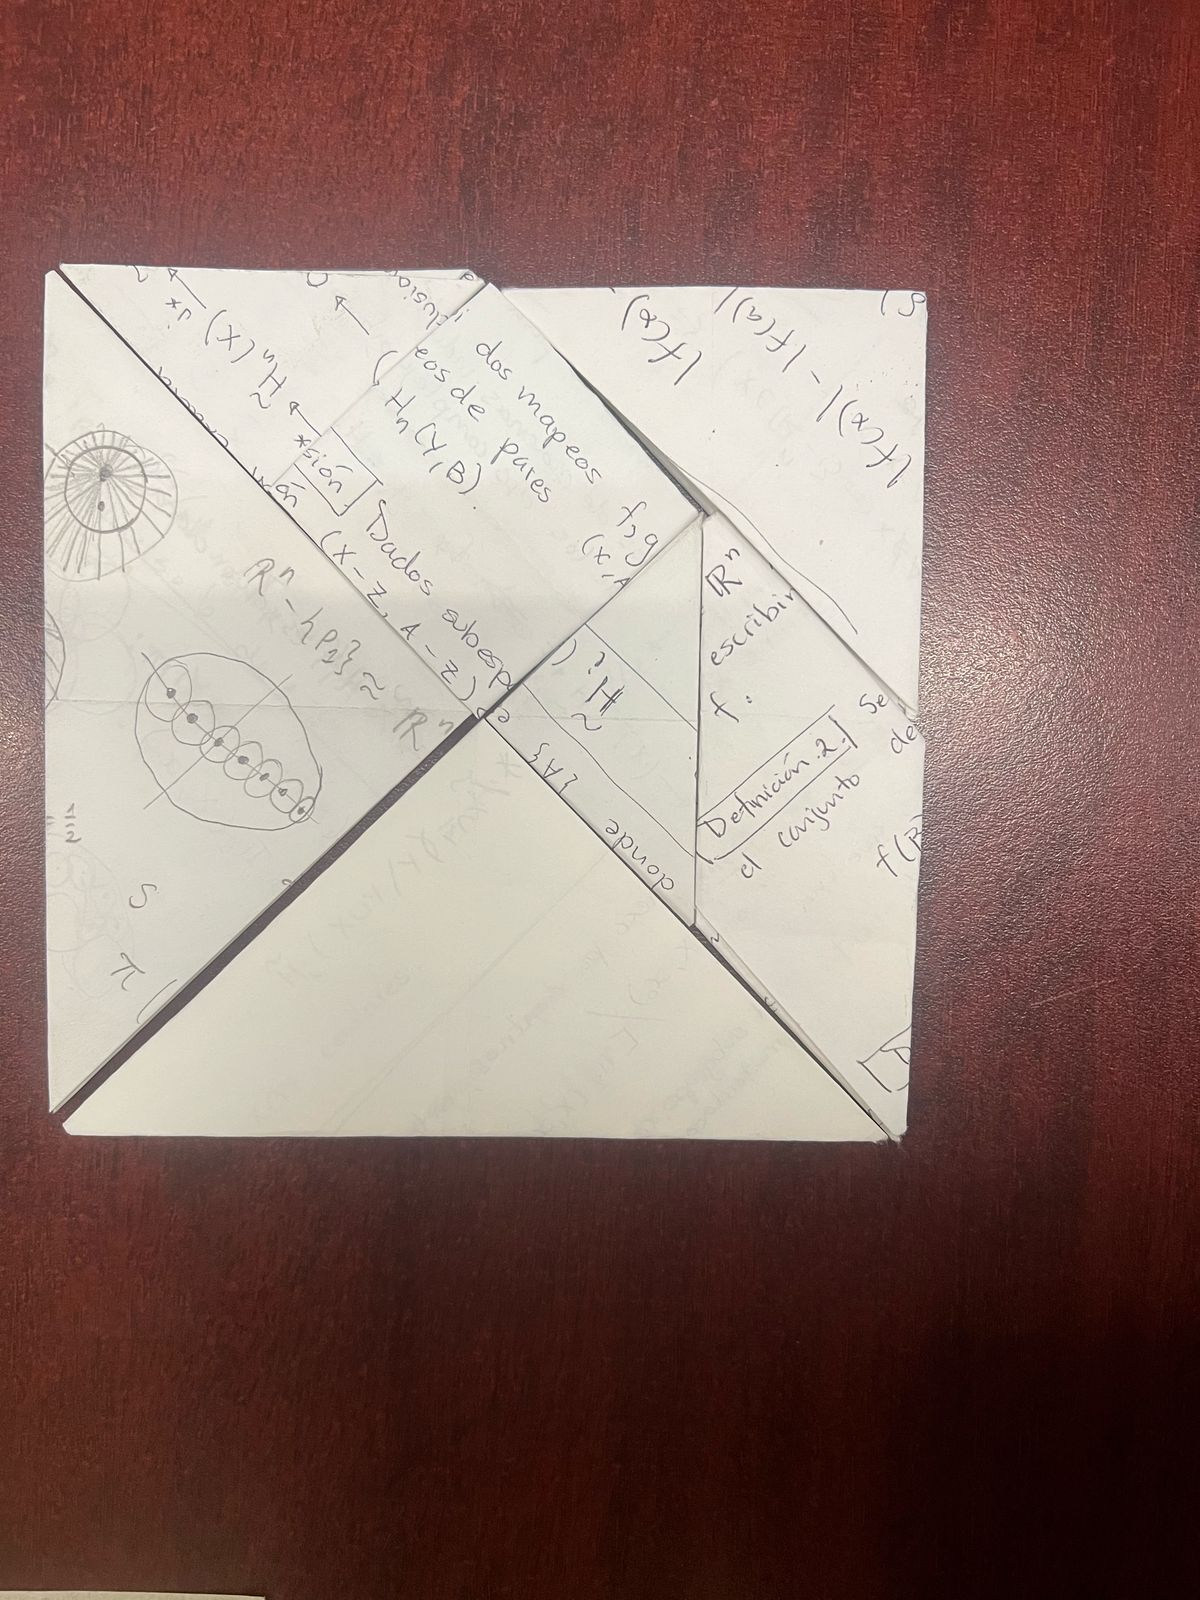
\includegraphics[scale=0.05]{clases/images/cuadrado.jpeg} & 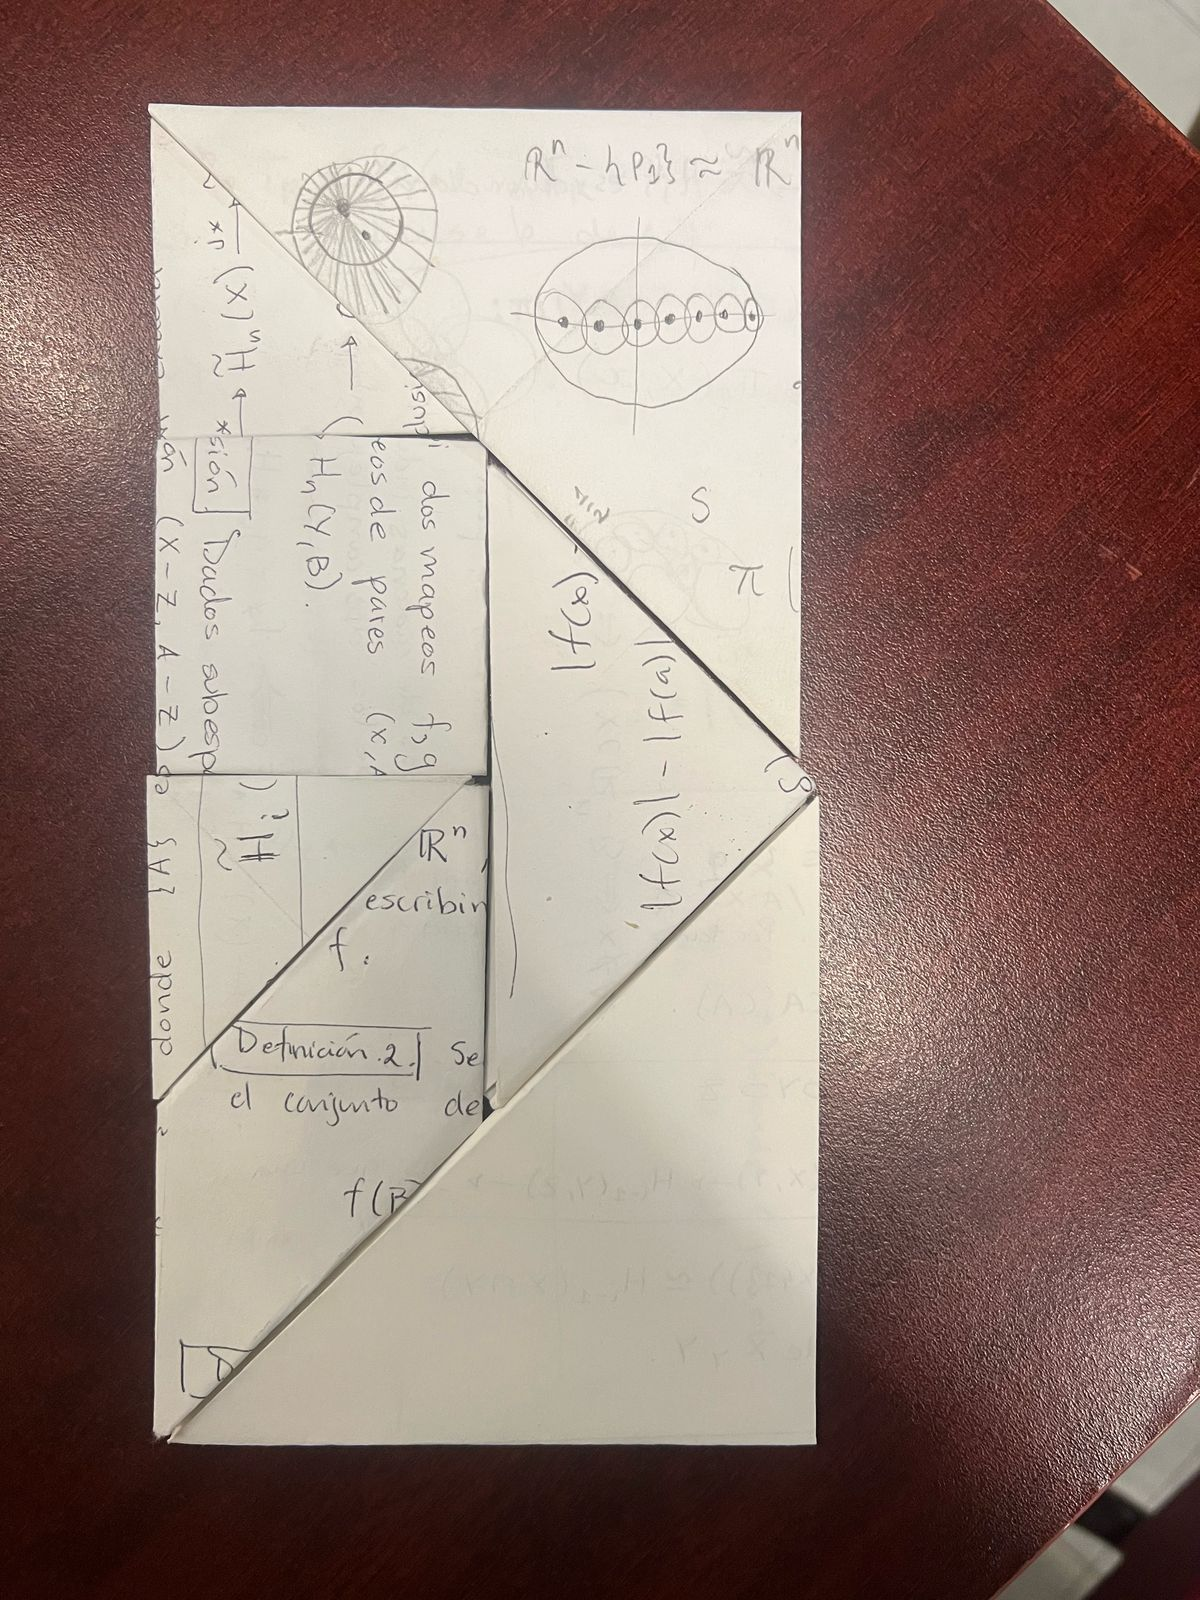
\includegraphics[scale=0.05]{clases/images/rectangulo.jpeg} & &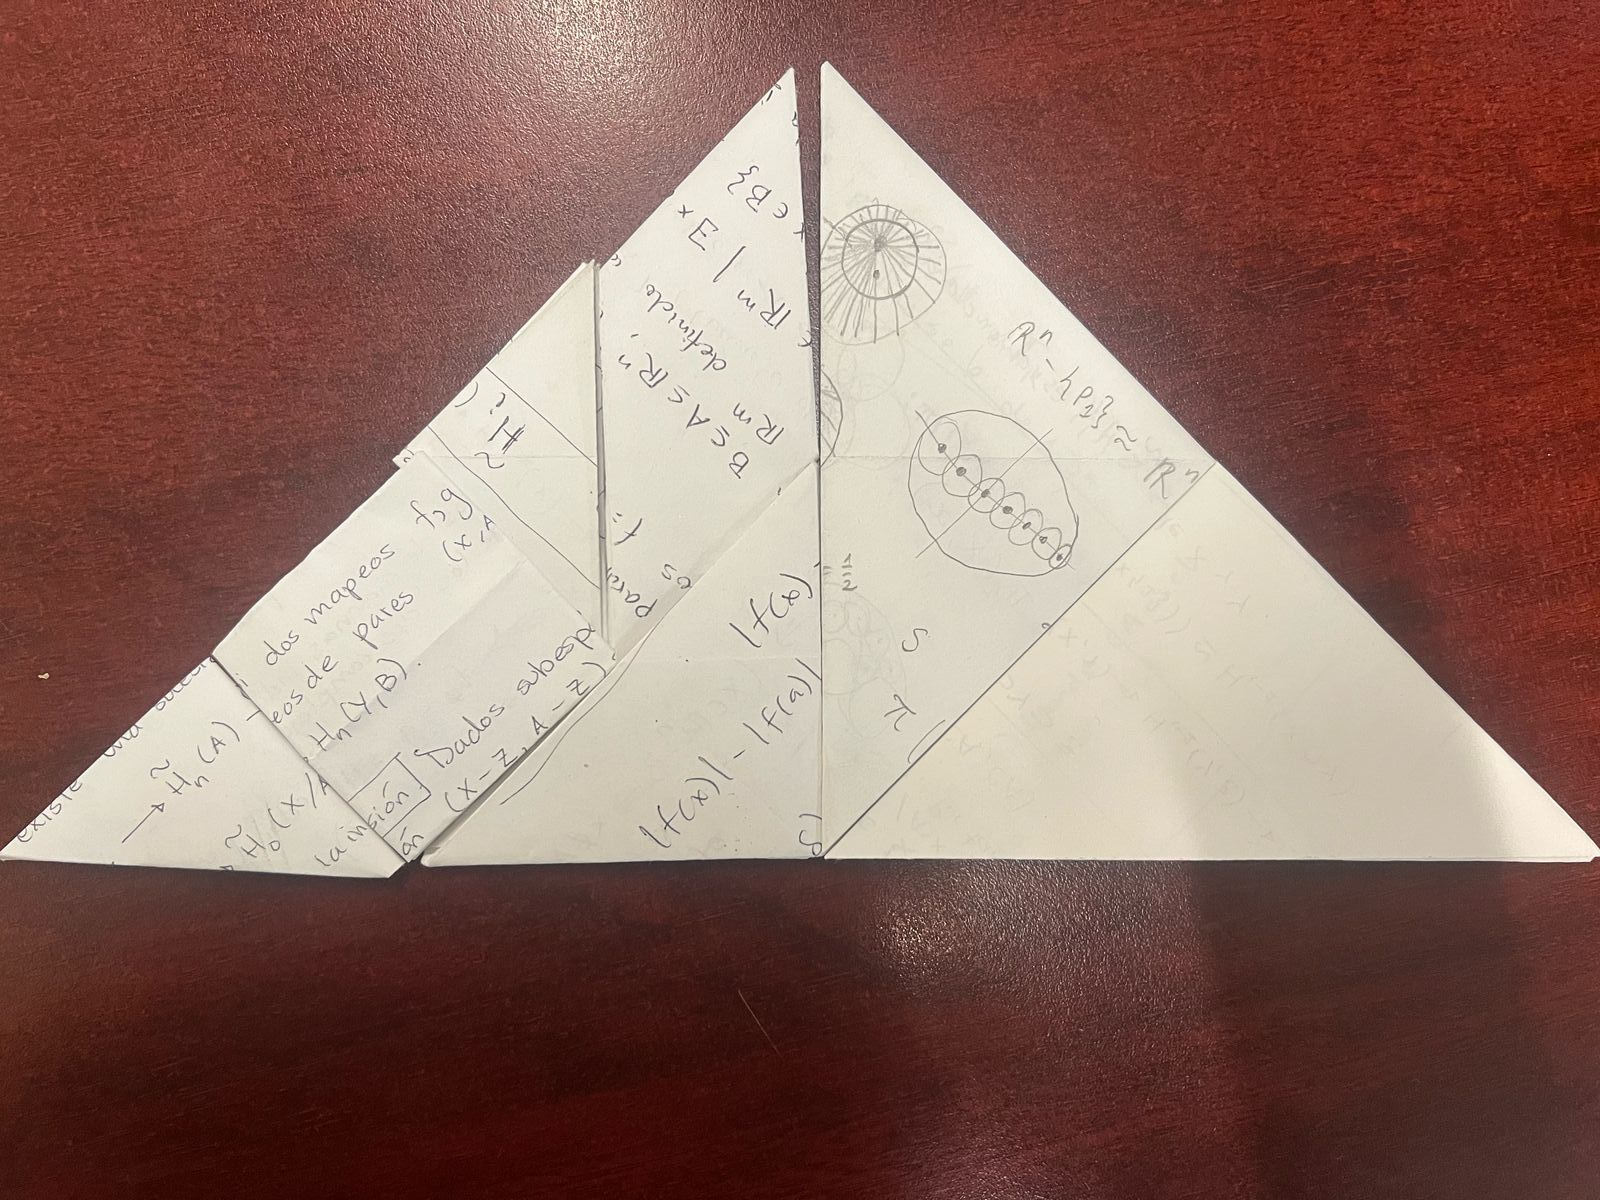
\includegraphics[scale=0.05]{clases/images/equilatero.jpeg} & 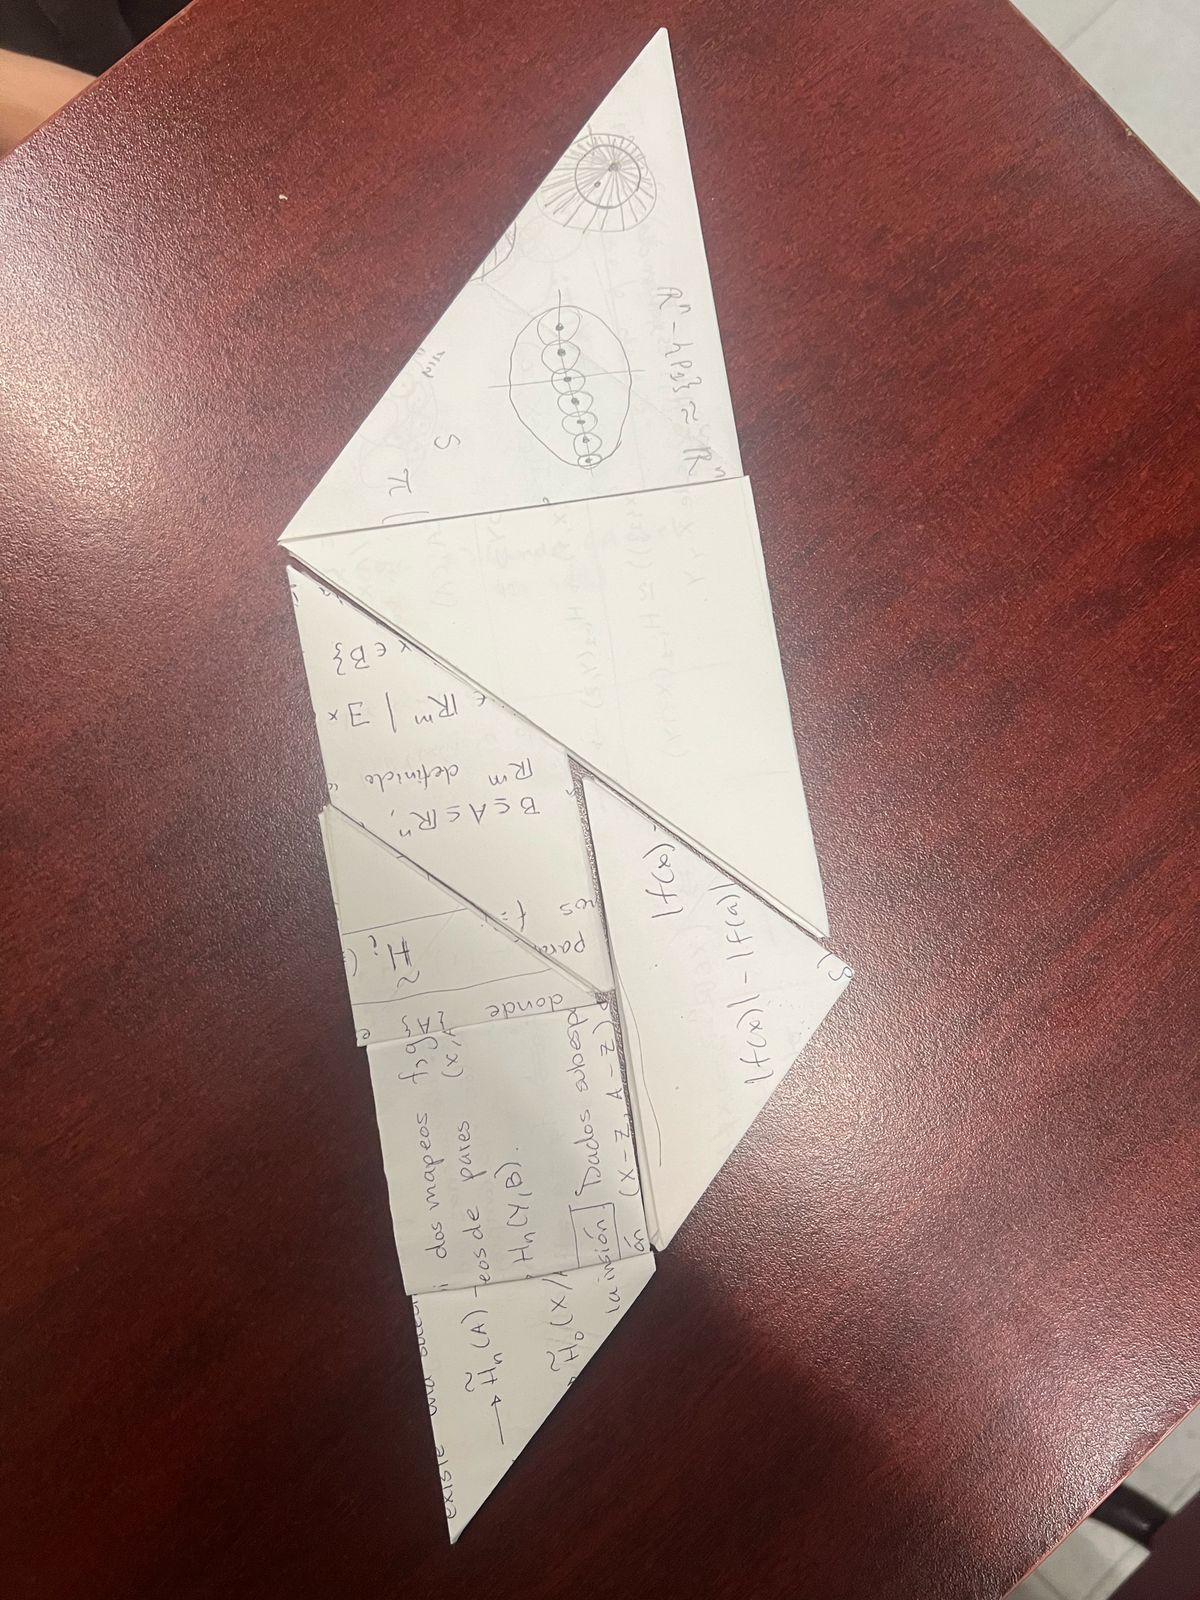
\includegraphics[scale=0.05]{clases/images/rombo.jpeg} \\ \hline
    
            \end{tabular}        
    }

La forma en que realizamos cada figura fue comenzando con el cuadrado, a partir de él, buscando mover la menor cantidad de piezas para poder construir el resto de figuras, recordando que toda figura tienen una triangulación.
    
\end{itemize}
  %\chapter{Clase 3. Tangram circular y problemas}
\textbf{13/02/2025}
\section{Tangram circular}

Los materiales y herramientas necesarias para el tangram circular fueron:
    \begin{itemize}
        
        \item Rectangulo de fomi
        \item Regla
        \item Compás
        \item Lápiz
        
    \end{itemize}

Elaboración:
    \begin{enumerate}
        
        \item Coloca la hoja en horizontal y traza $l_1$ de forma vertical de modo que divida el fomi en dos partes y una de ellas sea de $\frac{2}{3}$ del tamaño total del largo
        \item Traza $l_2 \perp l_1$ dividiéndola en dos mitades
        \item Con el compás, traza $C(O,r)$ donde $O = l_1 \cap l_2$
        \item Sean $A,B \in l_1$ en lados opuestos de $l_2$ tal que  estos puntos son las intersecciones de $C(O,r)$ con $l_1$ y análogamente para $C,D \in l_2$ (Sea $C$ elemento del lado de $l_1$ de mayor longitud)
        
         \item Traza los segmentos $\overleftrightarrow{AC}$ y $\overleftrightarrow{BC}$
         \item Abre el compás al tamaño del diámetro y traza dos arcos de circunferencia iniciando el trazo desde el punto $A$ y el segundo en $B$ de modo que ambos interseccten $l_2$ en el lado de $l_1$ que contiene a C
         \item Sea $E$ la intersección de $\overleftrightarrow{AC}$ con el arco de circunferencia que pasa por $A$. análogamente para $F$
         \item Traza una circunferencia $C'(C,r'')$ donde $r'' = CF $

         \item Traza otra circunferencia $C'(D,r'')$ y sean $G,H$ los puntos de intersección de $C'(D,r'')$ con $l_1$
         \item Traza los segmentos $\overline{DG}$ $\overline{DH}$
      \end{enumerate}

Las figuras trazadas deben quedar como la siguiente imagen
\begin{center}
   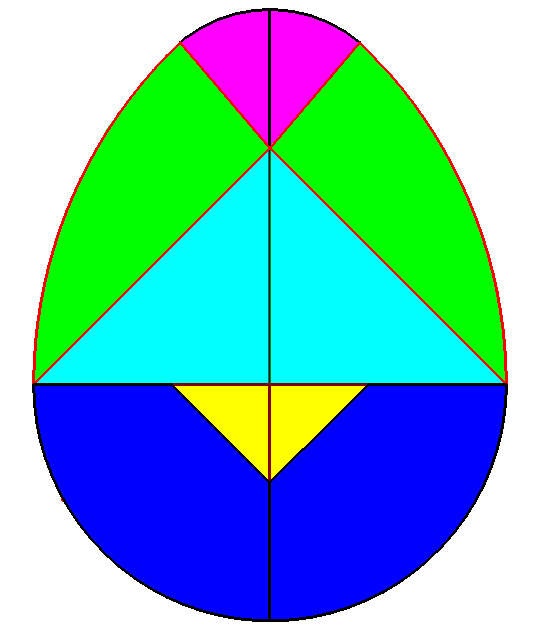
\includegraphics[scale=0.05]{clases/images/huevodecolon.jpg}
\end{center}

Despues de realizar el tangram, se debían hacer ciertas figuras que mostró la maestra en clase, de las cuales una se hizo en clase y la otra quedó de tarea.

\begin{center}
   \begin{tabular}{ccc}
      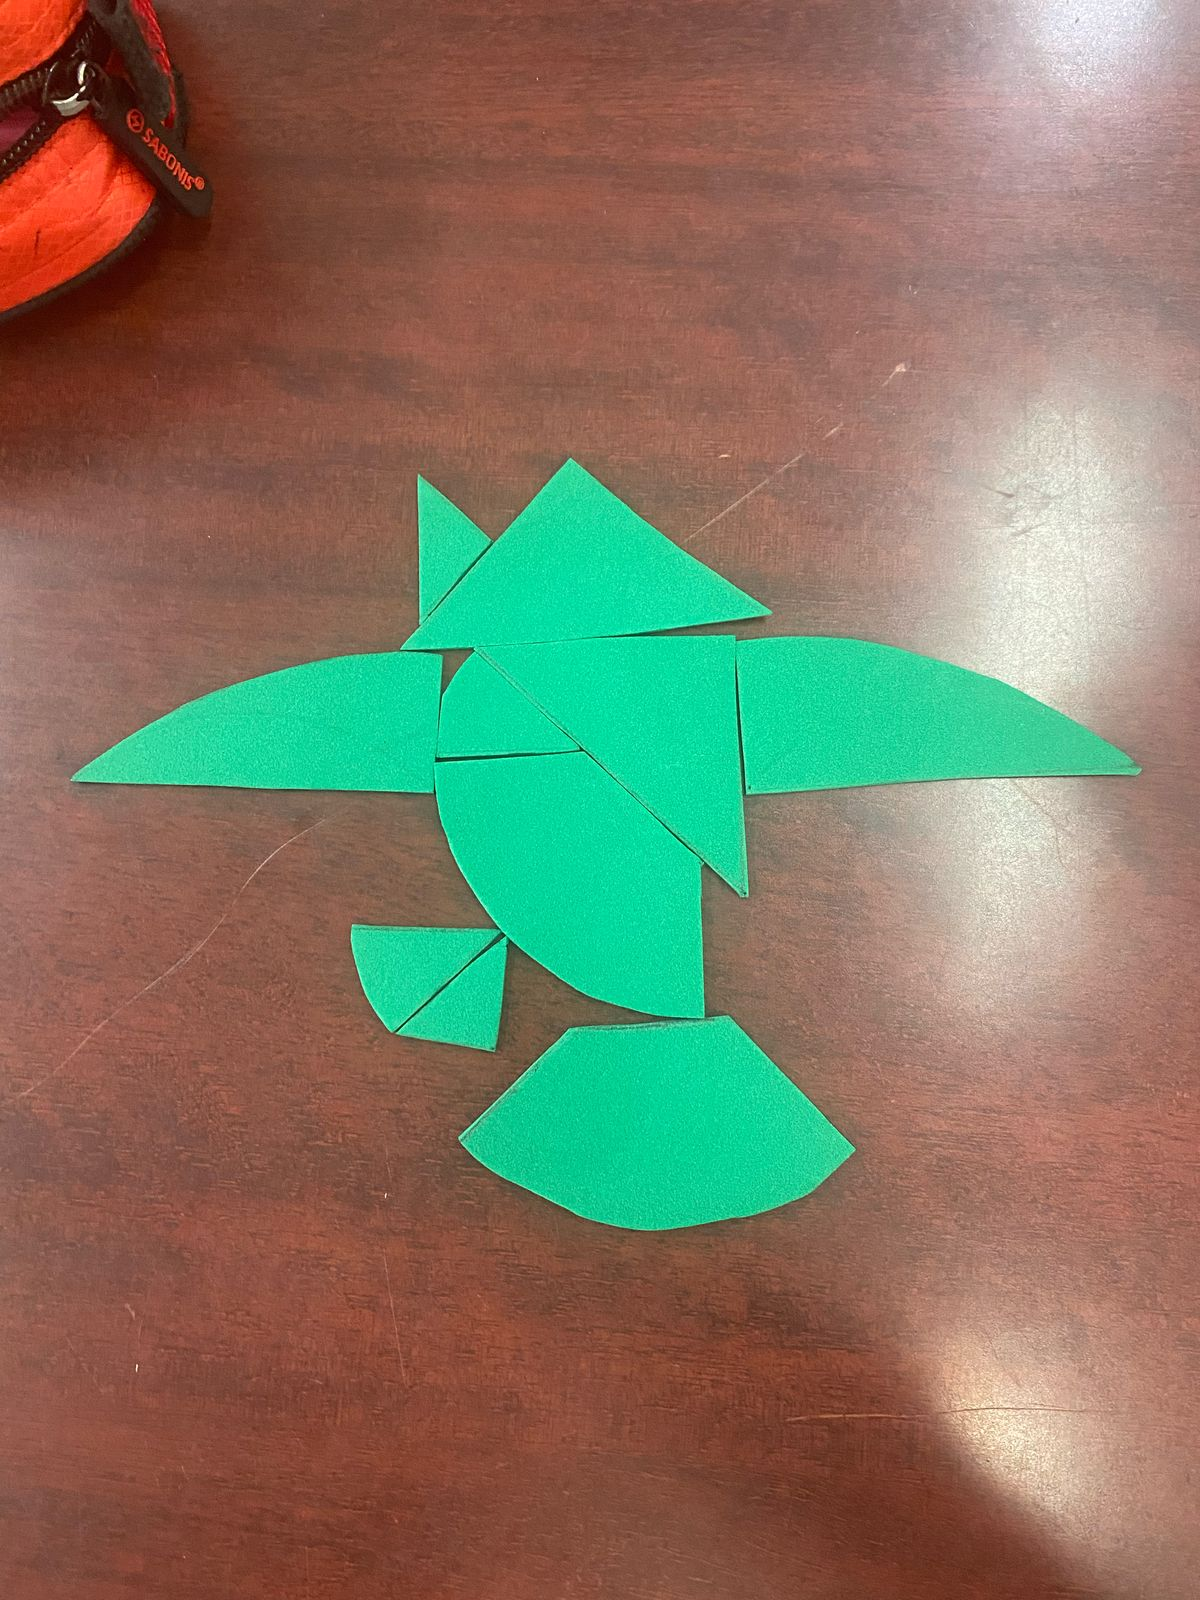
\includegraphics[scale=0.09]{clases/images/clase3/Pajaro.jpeg}&&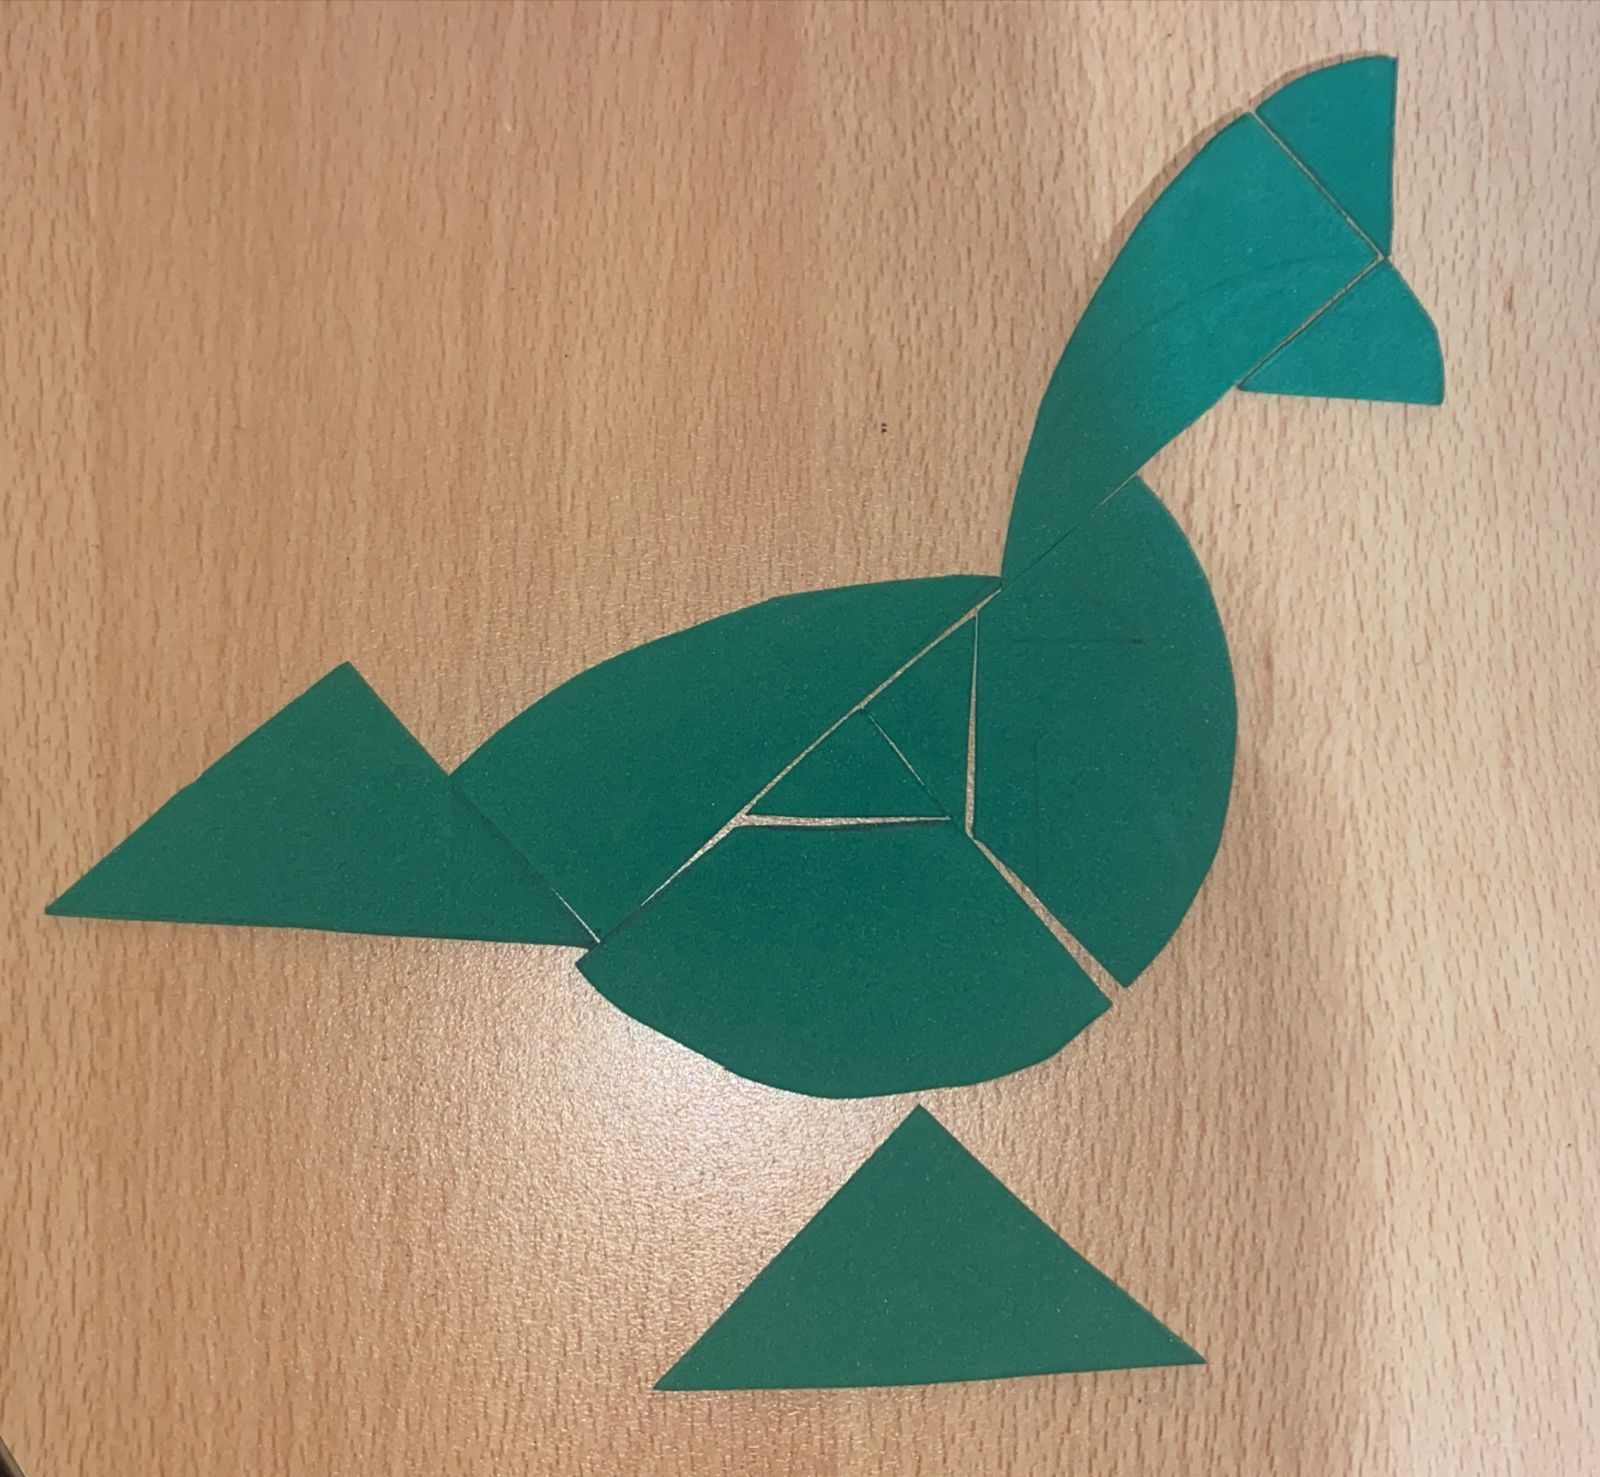
\includegraphics[scale=0.09]{clases/images/clase3/Pajaro2.jpeg}
   \end{tabular}
\end{center}

La manera en como resolví el problema fue analizando cada borde de mis piezas de tangram contra los bordes de las figuras a realizar, acomodando primero las piezas que parecían más faciles por estar a simple vista sin necesidad de unirles más piezas.

\section{Acertijos}\label{sec:C3ACERTIJOS}

\begin{ejem}\label{ejem:c3P1}
   Un campesino lleva al mercado para vender un lobo, una cabra y un repollo; al marchar así con su mercancía debe poner cuidado en que el lobo no ataque a la cabra y que la cabra no se coma el repollo.
   Se encuentra con un río que le conviene cruzar de esta manera: como no puede ni debe hacer pasar al mismo tiempo más de una cosa que con-duce, ha de poner cuidado en que el lobo en ausencia del campesino no pueda atacar a la cabra ni la cabra comerse el repollo, puesto que si él no está siempre presente la cabra comerá el repollo o será comida por el lobo. Cabe preguntarse entonces cómo podría hacer pasar sus mercaderías al otro lado del río sin sufrir ningún daño
\end{ejem}
   \textbf{SOLUCION.}Primero el campesino debe de cruzar a la cabra, después la deja del otro lado regresa y se lleva ya sea el lobo o el repollo, (en este caso tomaremos al repollo) cuando llega al mismo lado de la cabra, deja el repollo y en su regreso lleva consigo a la cabra y al momento de llegar con el lobo, deja la cabra en el lado inicial,  y se lleva al lobo para dejarlo al mismo lado que el repollo y al momento de regresar nuevamente cruza a la cabra. Así, el campesino habrá cruzado a los tres, sin que la cabra o el repollo sean comidos.

\begin{ejem}\label{ejem:c3P2}
   Un herrero debe formar una cadena con 15 eslabones y tiene a la mano 5 trozos de cadena con 3 eslabones cada uno. ¿Cuál es la cantidad mínima de eslabones que debe romper y soldar? Para lograr su objetivo.
\end{ejem}
   \textbf{SOLUCIÓN.}El herrero rompe 4 trozos de eslabones por alguno de los extremos de ellos y los solda al otro conjunto de eslabones en el extremo en el cual no fue roto ninguno

\begin{ejem}\label{ejem:c3P3}
   Tienes 9 monedas aparentemente idénticas, pero una de ellas es falsa y pesa más que las demás. Dispones de una balanza de dos platillos y puedes realizar solo dos pesajes para identificar cuál es la moneda falsa. ¿Cómo puedes determinar cuál es la moneda falsa bajo las condiciones pedidas?
\end{ejem}
   \textbf{SOLUCIÓN.}Primero se hacen tres grupos de tres monedas cada uno. Luego se toman dos grupos al azar y se pesan a partir de aquí tenemos dos casos:
   \begin{enumerate}
      \item La balanza se mantiene equilibrada.
      \item La balanza no se mantiene equilibrada
   \end{enumerate}
   En el caso uno podemos deducir que la moneda falsa está en el tercer grupo que no fue pesado y y de este mismo grupo se toman dos monedas y nuevamente hay dos casos, el primero en donde ambas monedas están equilibradas, esto nos indica que la moneda falsa es aquella que no fue pesada, y el segundo caso es aquel en donde una moneda pesa más que la otra.
   Para el segundo caso en donde la balanza no se mantuvo equilibrada, se toma el grupo que pesó más y la moneda falsa se halla de manera análoga al primer caso.

\begin{ejem}\label{ejem:c3P4}
   Un hombre vende vino pero sólo dispone de una medida de tres litros. Llega al negocio otro hombre que lleva una medida de cinco litros y que pide al tabernero cuatro litros de vino; la cuestión es saber cómo podrá el tabernero dar al cliente esos cuatro litros puesto que solo tiene un jarro de tres litros en tanto que el jarro del cliente es de cinco litros.
\end{ejem}
   \textbf{SOLUCIÓN.}Primero llenas la medida de 3l ,luego la vacías en la medida de cinco y nuevamente hasta que se llenen los 5l,  pues en la medida de tres quedará uno. Después de esto se desecha el vino de la medida de 5l y el litro de la jarra de tres se vierte en la medida más grande se vuelve a llenar la jarra de 3 l y se vacía en la de cinco obteniendo así, los 4l

\begin{ejem}\label{ejem:c3P5}
   Las monedas en la foto forman la punta de una flecha que apunta hacia arriba. Cambia de posición tres de ellas para obtener una punta de flecha que apunta hacia abajo.
   \begin{center}
      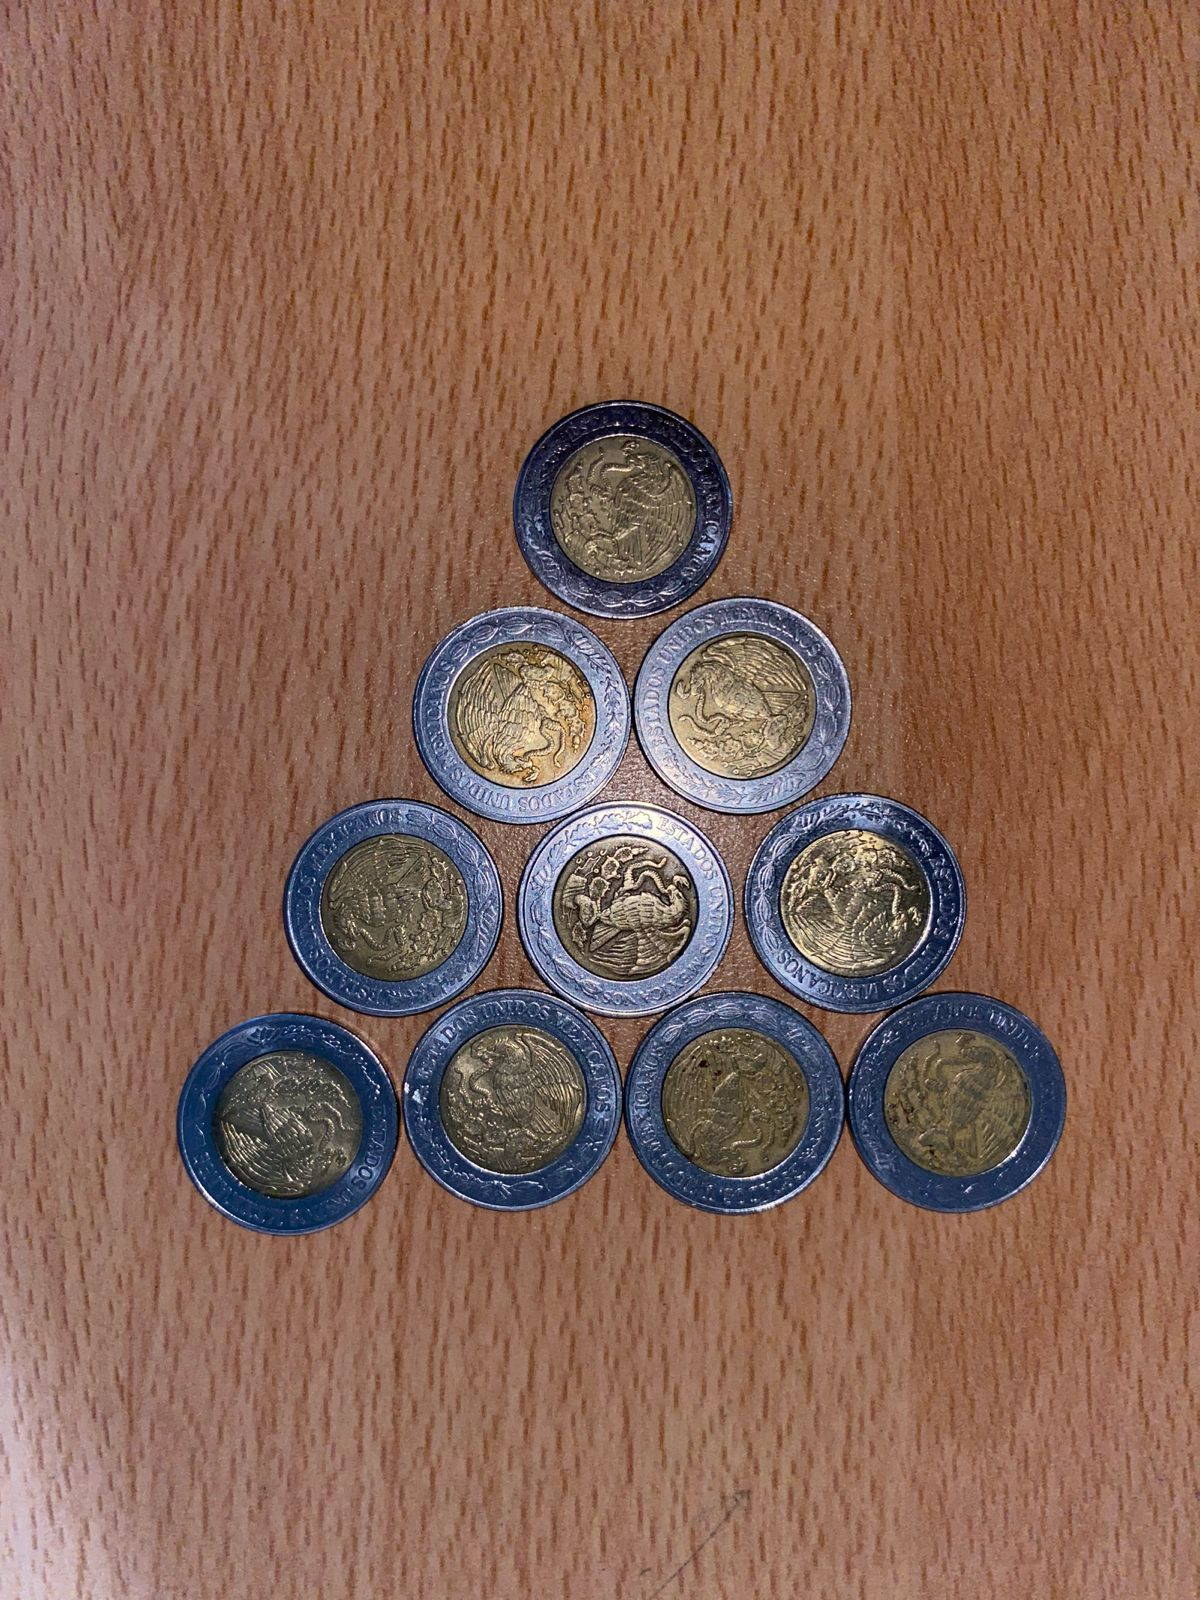
\includegraphics[scale=0.09]{clases/images/clase3/Flecha.jpeg}
   \end{center}
\end{ejem}
   \textbf{SOLUCIÓN 1.} Primero enumeramos cada fila de monedas, según la cantidad. Después de esto, observamos que la base debía tener cuatro monedas, por lo cual tomamos dos monedas de la fila cuatro, y las pasamos a la fila dos y la moneda de la fila, uno la pasamos debajo de la fila cuatro.
   \\
   \begin{center}
      
      \begin{tabular}{c c c}
            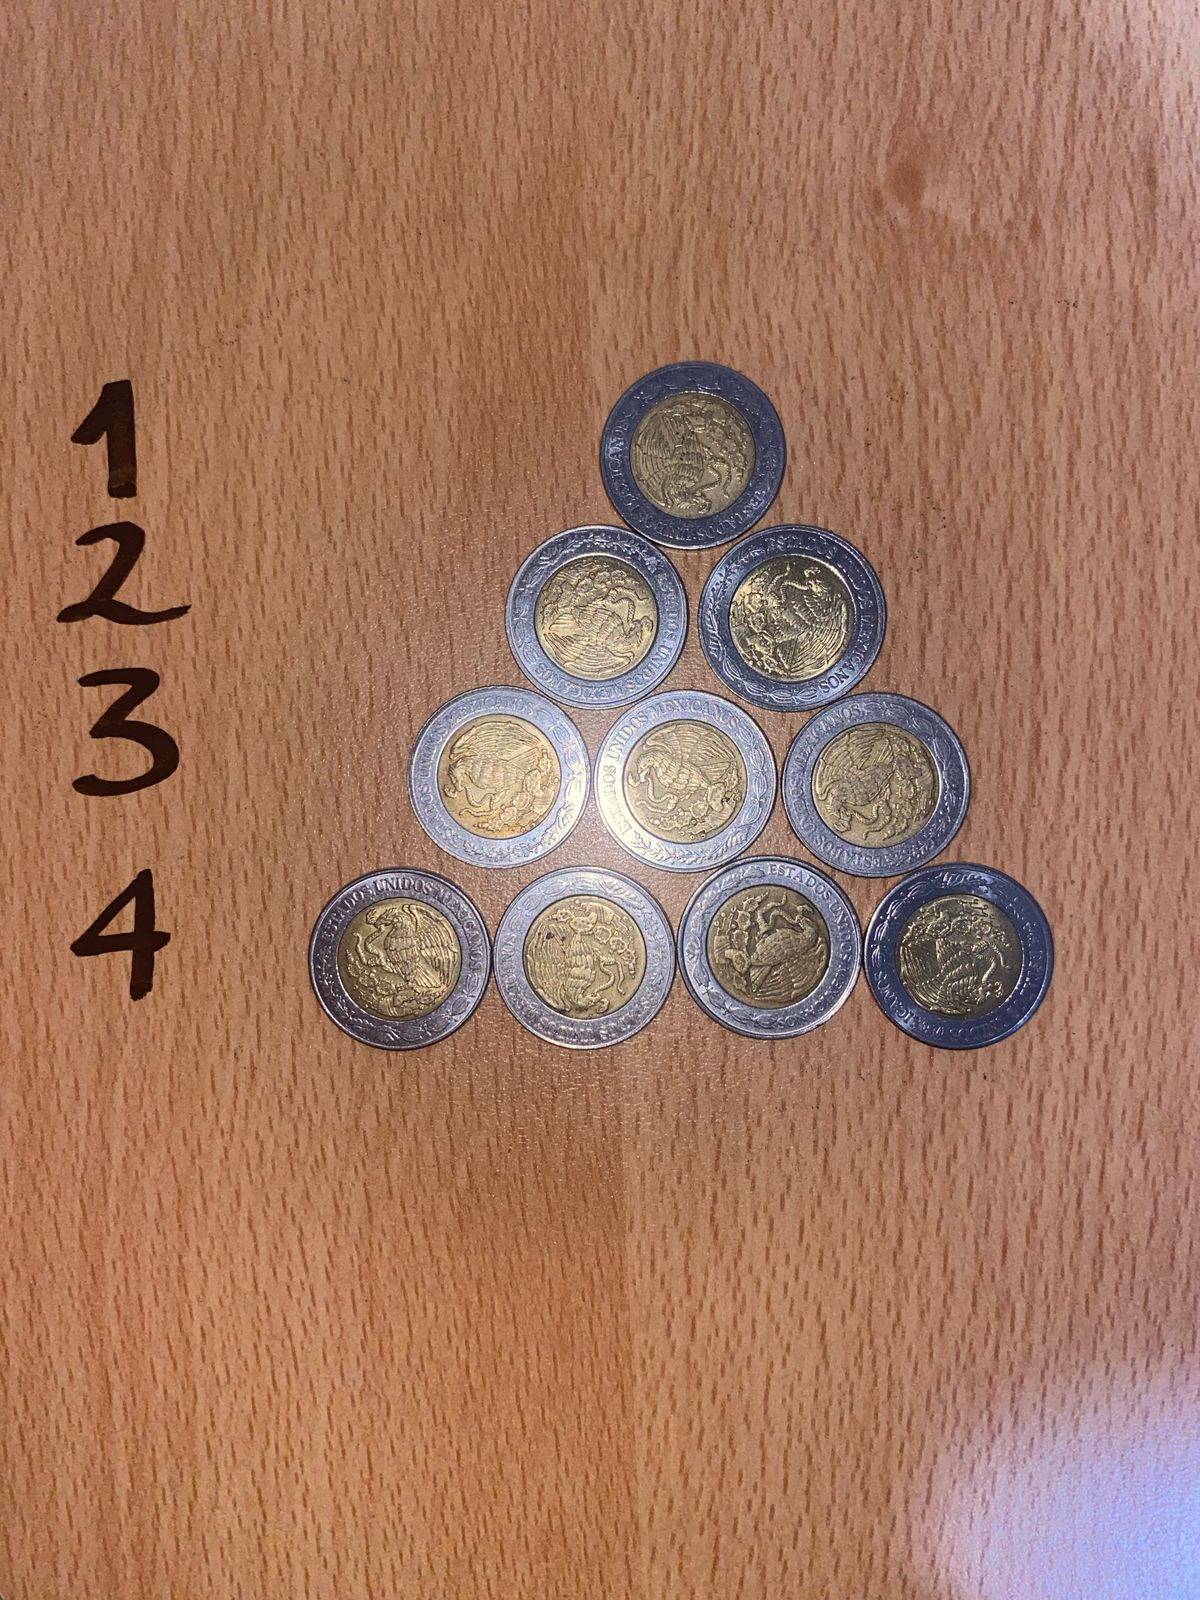
\includegraphics[scale=0.09]{clases/images/clase3/FlechaEnum.jpeg}&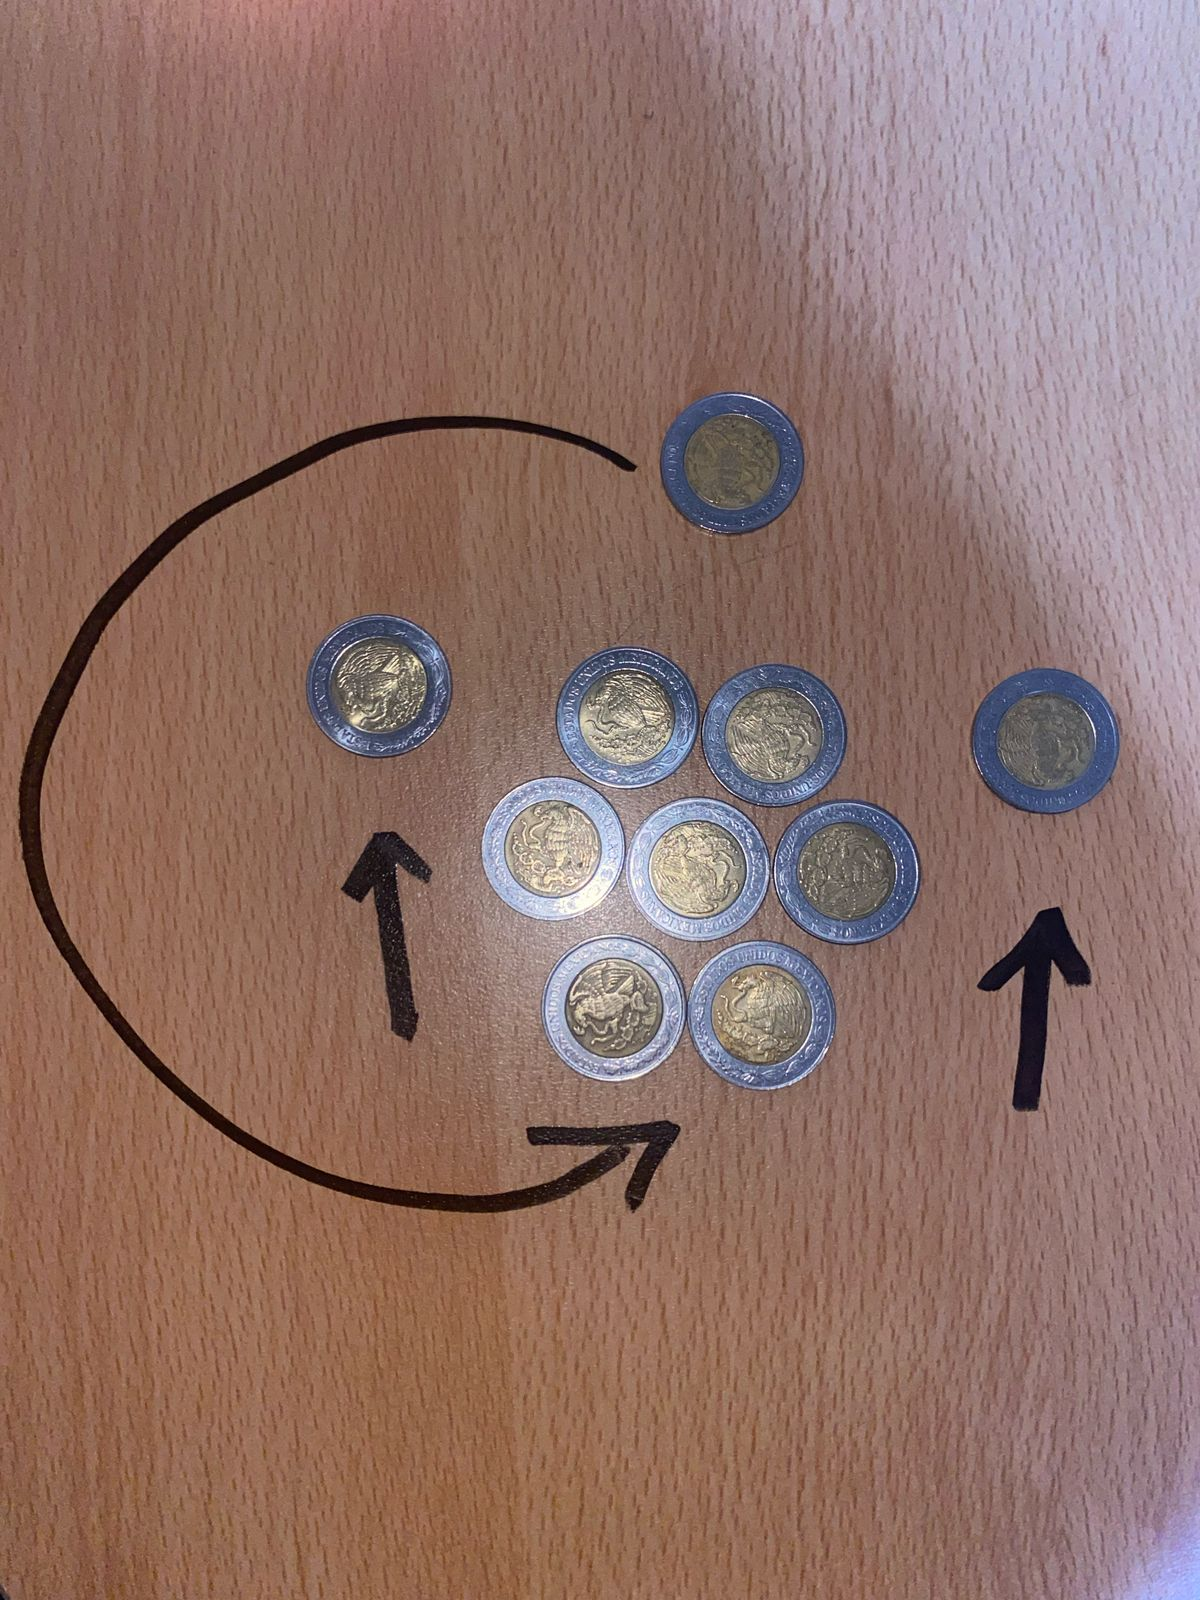
\includegraphics[scale=0.09]{clases/images/clase3/base4punta1.jpeg}&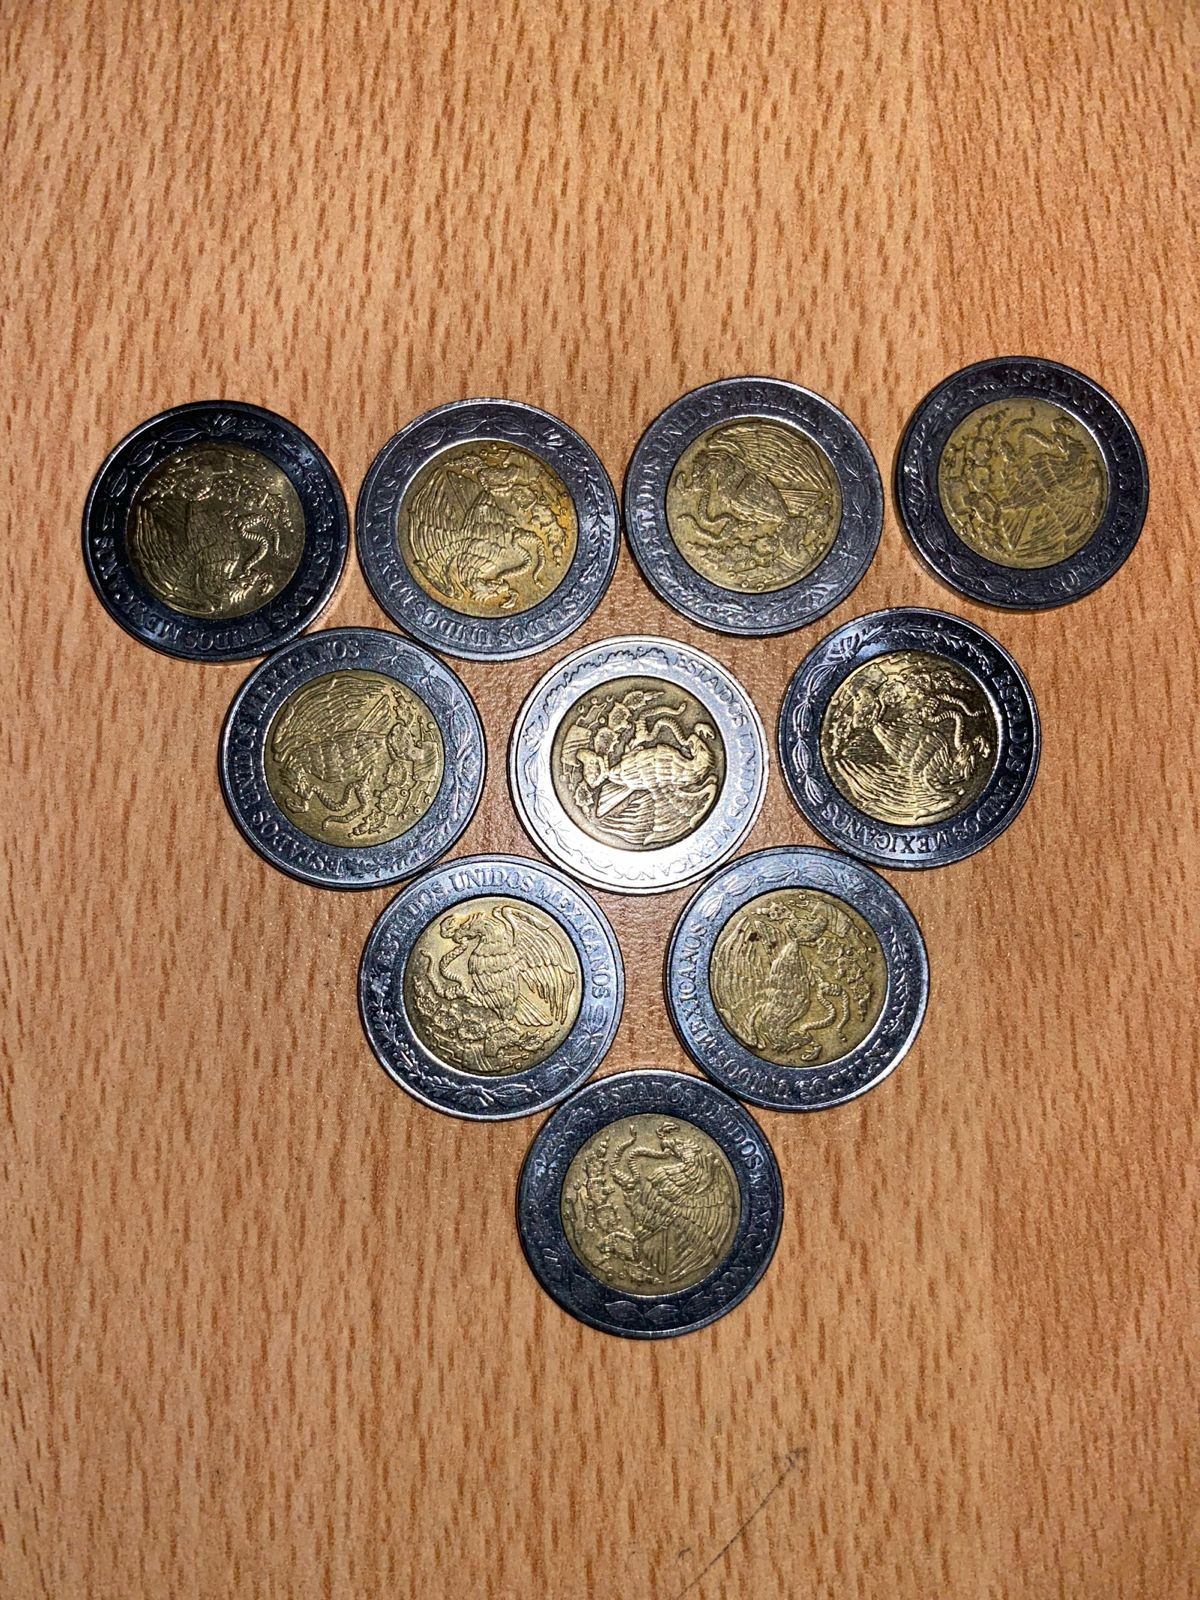
\includegraphics[scale=0.09]{clases/images/clase3/FlechaInvertida.jpeg}
      \end{tabular}

   \end{center}   

   \textbf{SOLUCIÓN 2.} La segunda solución que encontramos fue ver la foto de las monedas, como un triángulo y mover únicamente los vértices, dado que las otras monedas en ningún momento se movían al poner la punta de flecha en cualquier dirección cumpliendo así la regla de sólo mover tres monedas a la vez.

   \begin{center}
      
      \begin{tabular}{c c c}
            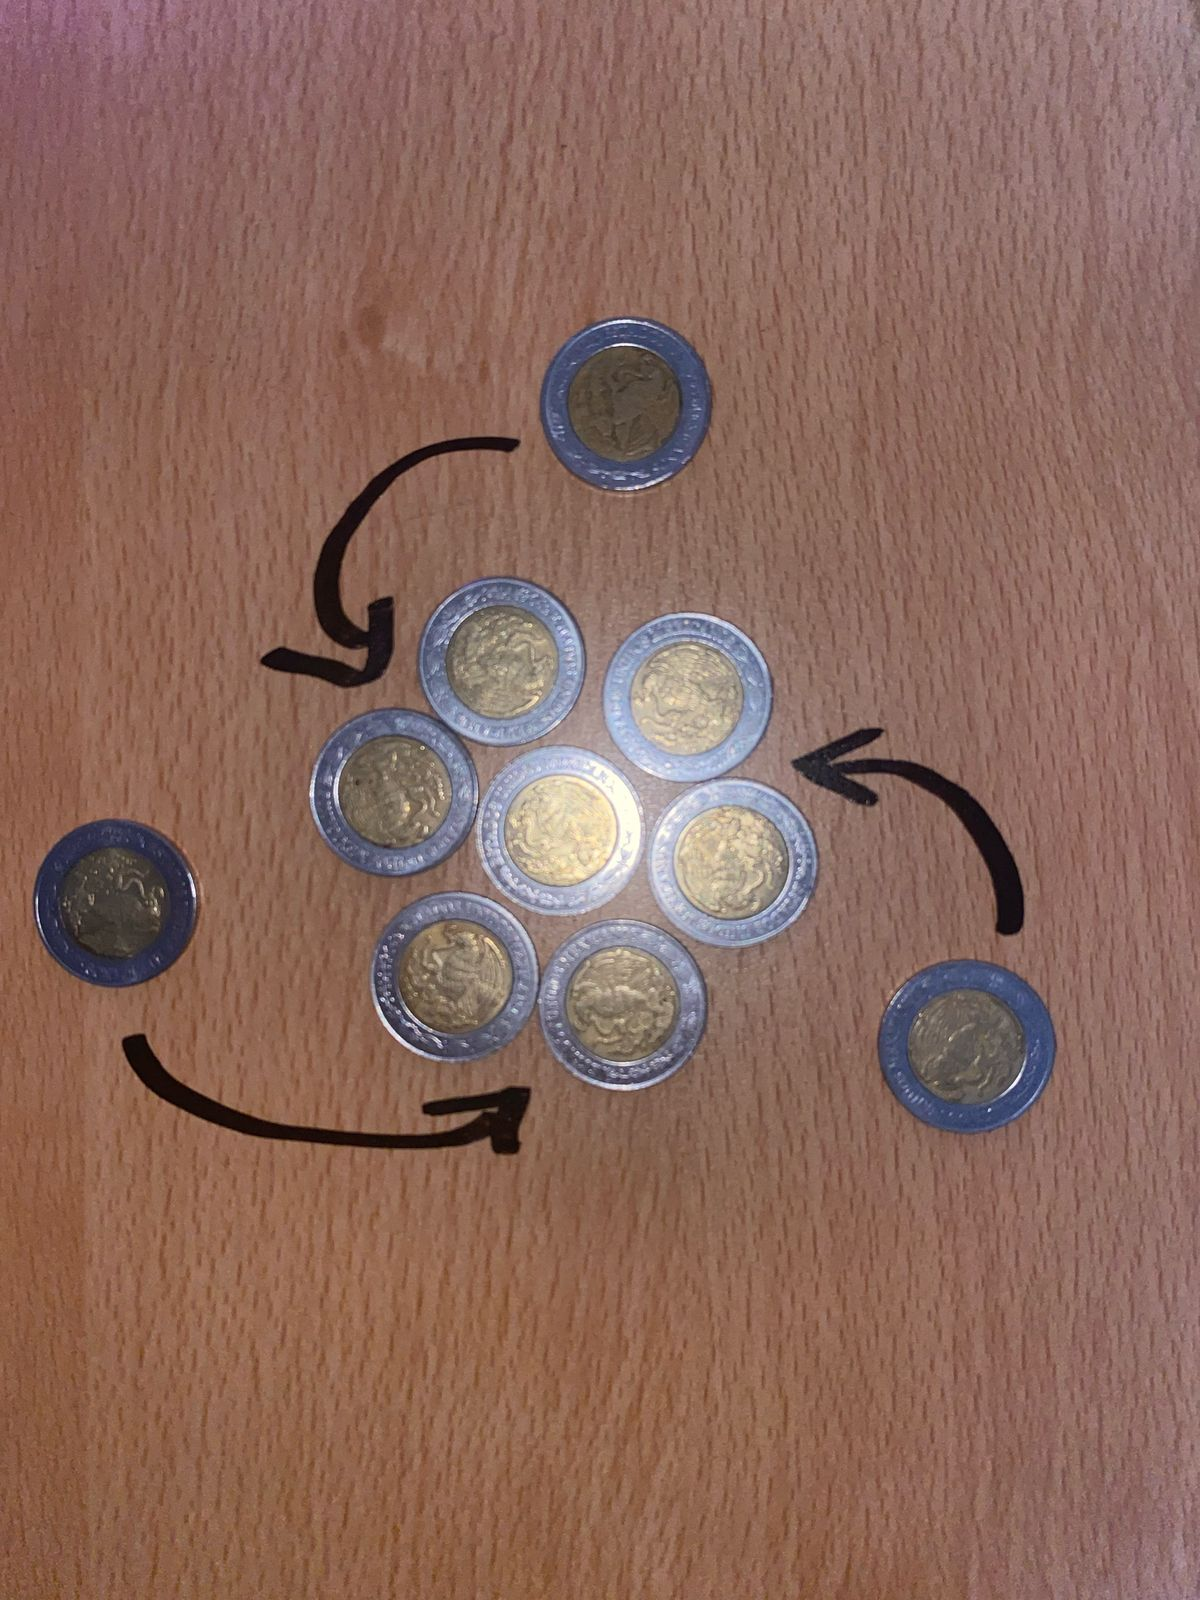
\includegraphics[scale=0.09]{clases/images/clase3/rotacionVertices.jpeg}&&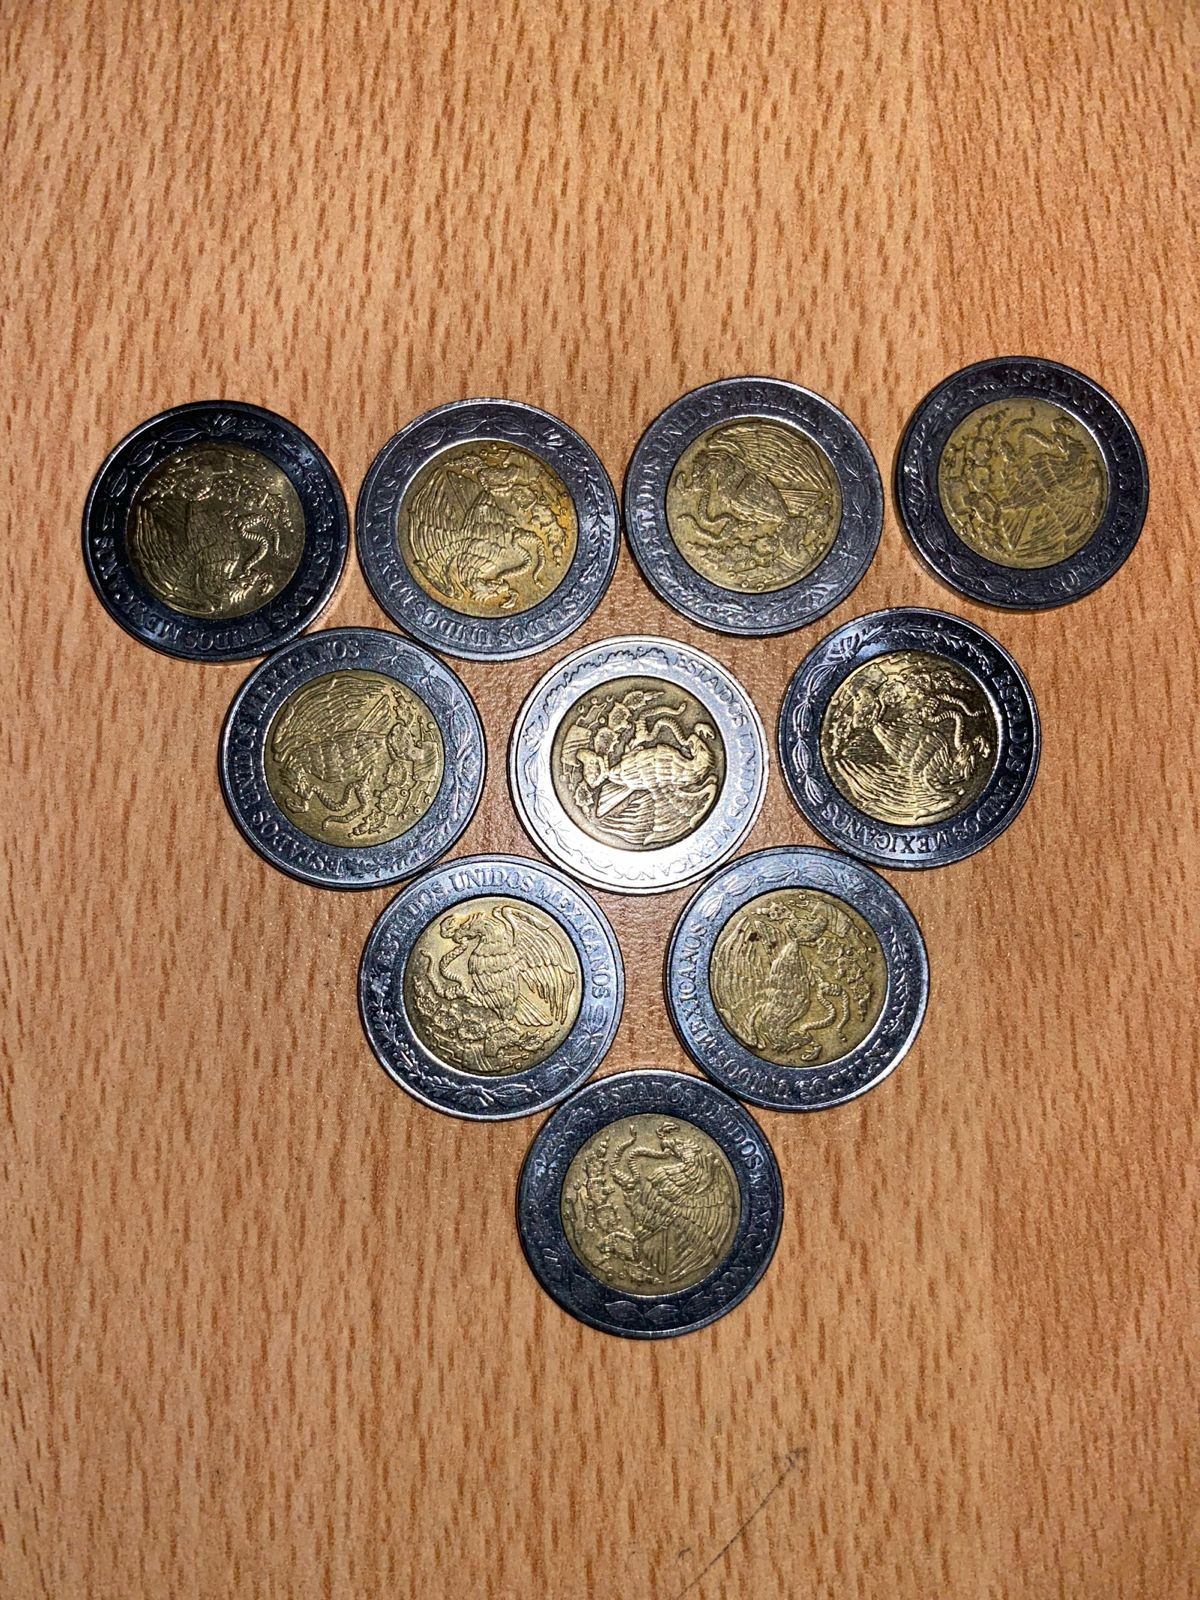
\includegraphics[scale=0.09]{clases/images/clase3/FlechaInvertida.jpeg}
      \end{tabular}
      
   \end{center}   
  %\chapter{Clase 4. Exposición de los problemas de la clase 3}
\textbf{18/02/2025}

Se formaron distintos equipos a la clase anterior y en algunos casos se plantearon resoluciones distintas a las que se habían llegado anteriormente, tanto en el equipo en el que me encontraba como en los que expusieron los demás problemas. 

Solo en los casos en los que se planteó una solución diferente a la que se llegó en la clase anterior serán mencionados, por lo tanto se podrá consultar la sección \hyperref[sec:C3ACERTIJOS]{acertijos} para ver las demás resoluciones.

\section{Problema 1}
\begin{figure}[h!]
    \begin{center}
        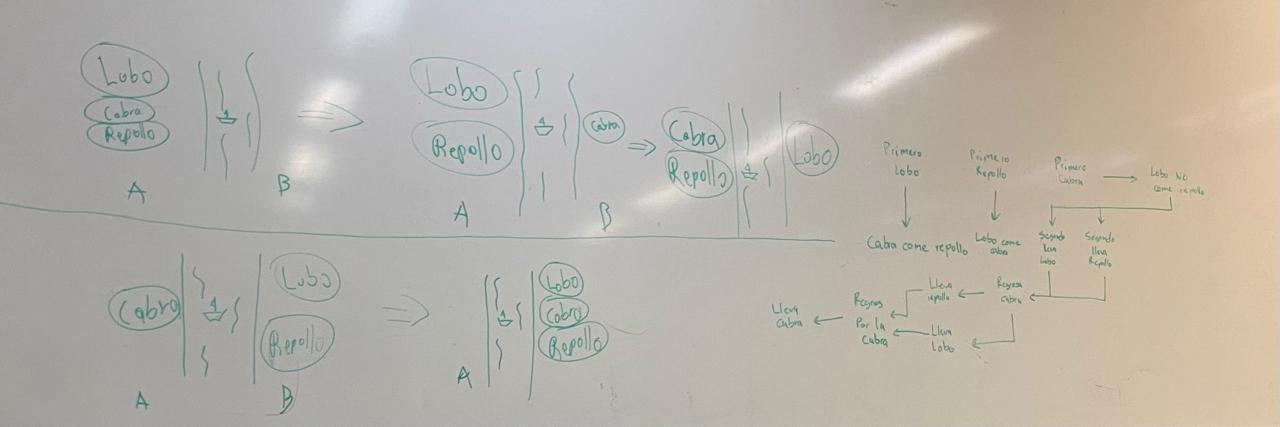
\includegraphics[scale=0.2]{clase4/problema1.jpeg}
    \end{center}
    \caption{Resolución al problema 2}
\end{figure}

\section{Problema 2}
La primera solución que plantearon fue la misma que a \hyperref[ejem:c3P2]{la anterior clase}, donde proponían romper cada trozo de cadena y lo representaron como una suma, pero luego utilizando el mismo método decidieron poner solo cuatro números 3 y cada signo mas representaría el quinto trozo de cadena, de este modo llegaron a la conclusión de que la cantidad mínima de eslabones a romper sería de 3.
\begin{figure}[h!]
    \begin{center}
        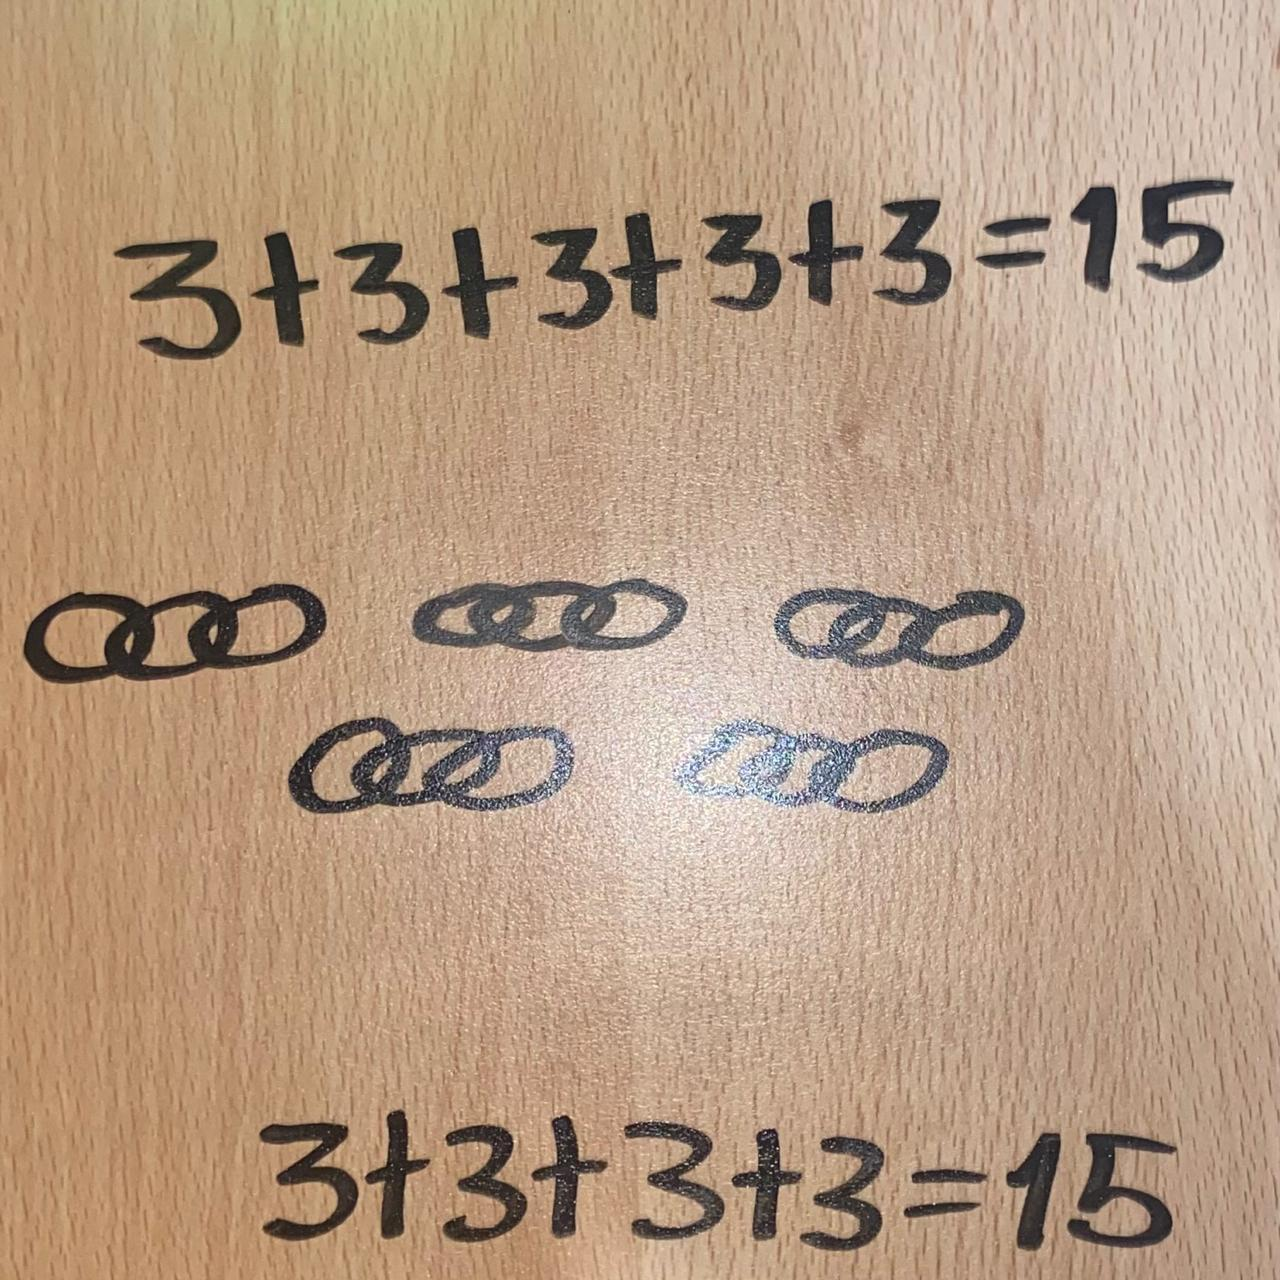
\includegraphics[scale=0.09]{clase4/problema2.jpeg}
    \end{center}
    \caption{Resolución al problema 2}
\end{figure}

\section{Problema 3}
\begin{figure}[h!]
    \begin{center}
        \begin{tabular}{cc}
            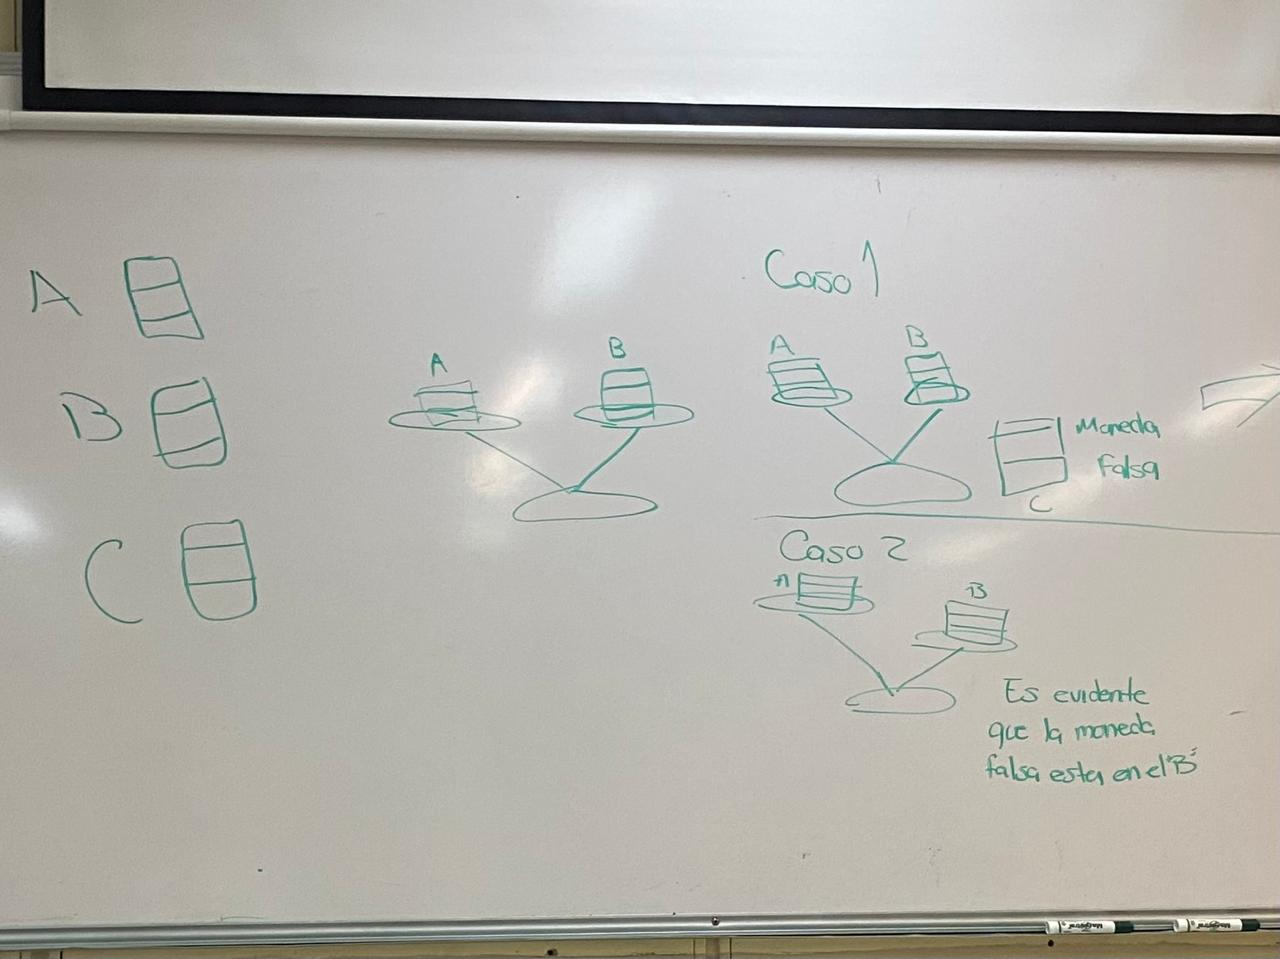
\includegraphics[scale=0.15]{clase4/problema3.1.jpeg}&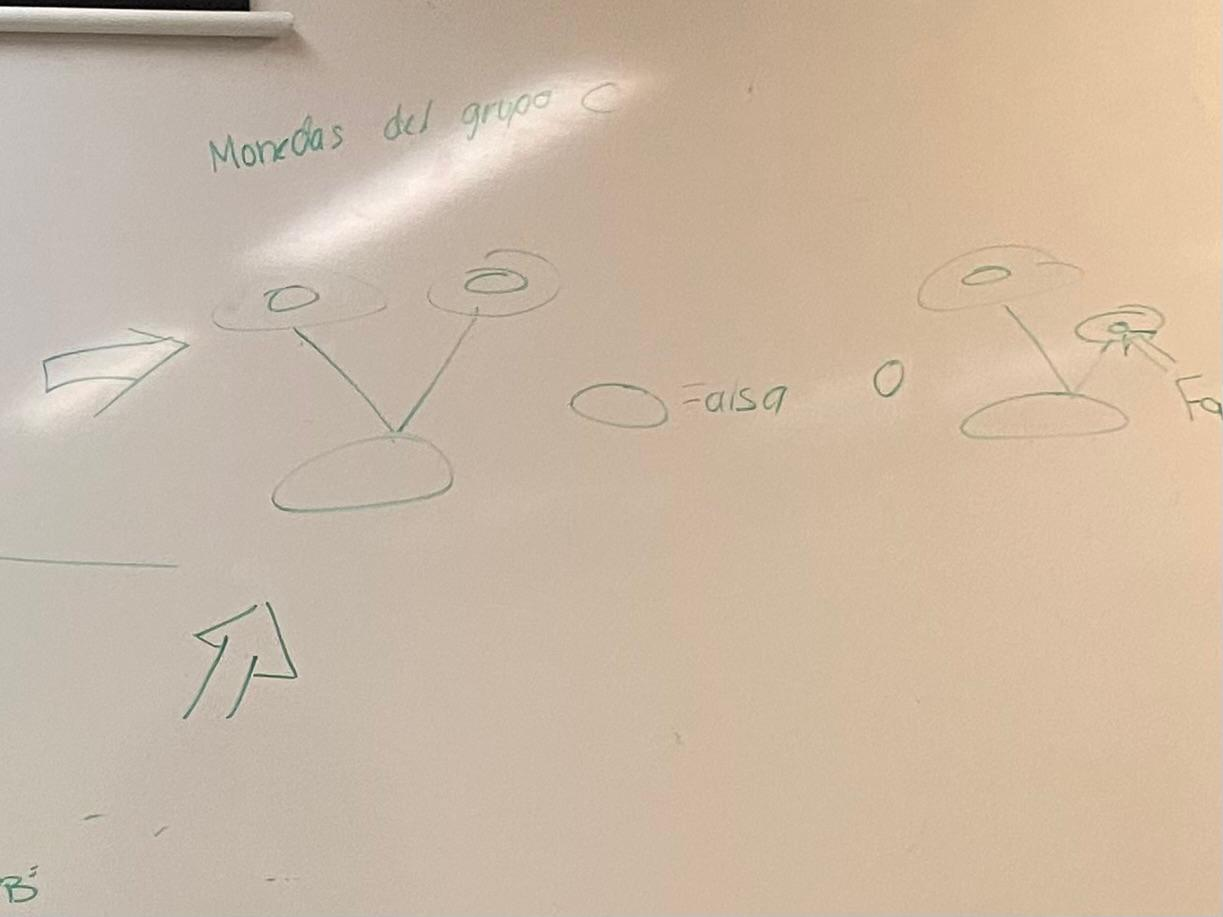
\includegraphics[scale=0.15]{clase4/problema3.2.jpeg}
        \end{tabular}
    \end{center}
    \caption{Resoluciónal al problema 3}
\end{figure}

\section{Problema 4}
La segunda solución la propuso un equipo diferente al que estaba exponiendo, pues el segundo caso que observaron los expositores, lo descartaron y otro equipo, y sólo la observación siguiente:
Después de llenar la jarra de 5 l, se pasaba 3 l a la jarra más pequeña y se descartaban, mientras que en la jarra más grande quedaban 2 l los cuales nuevamente se pasaban a la jarra más chica y por última vez se llenaba la jarra de cinco y se vertía 1 l en la jarra de tres, quedando así 4 l en la jarra más grande. Este es un caso similar al planteado en la anterior clase.

\begin{figure}[h!]
    \caption{Resolución al problema 4}
    \begin{center}
        \begin{tabular}{cccc}
            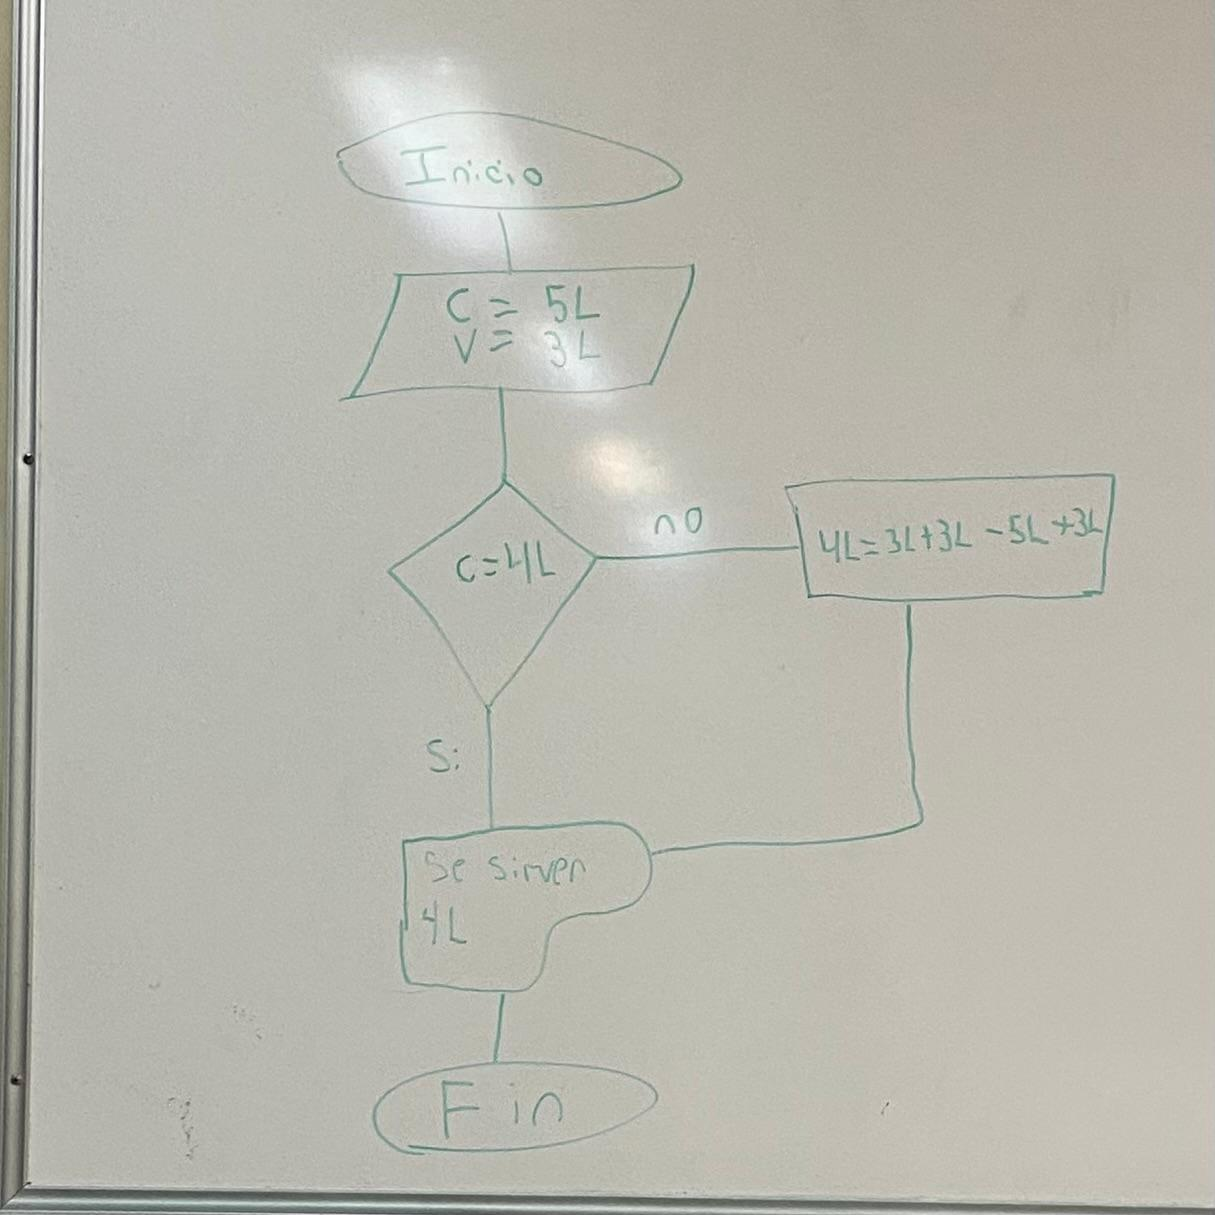
\includegraphics[scale=0.09]{clase4/problema4.1.jpeg}&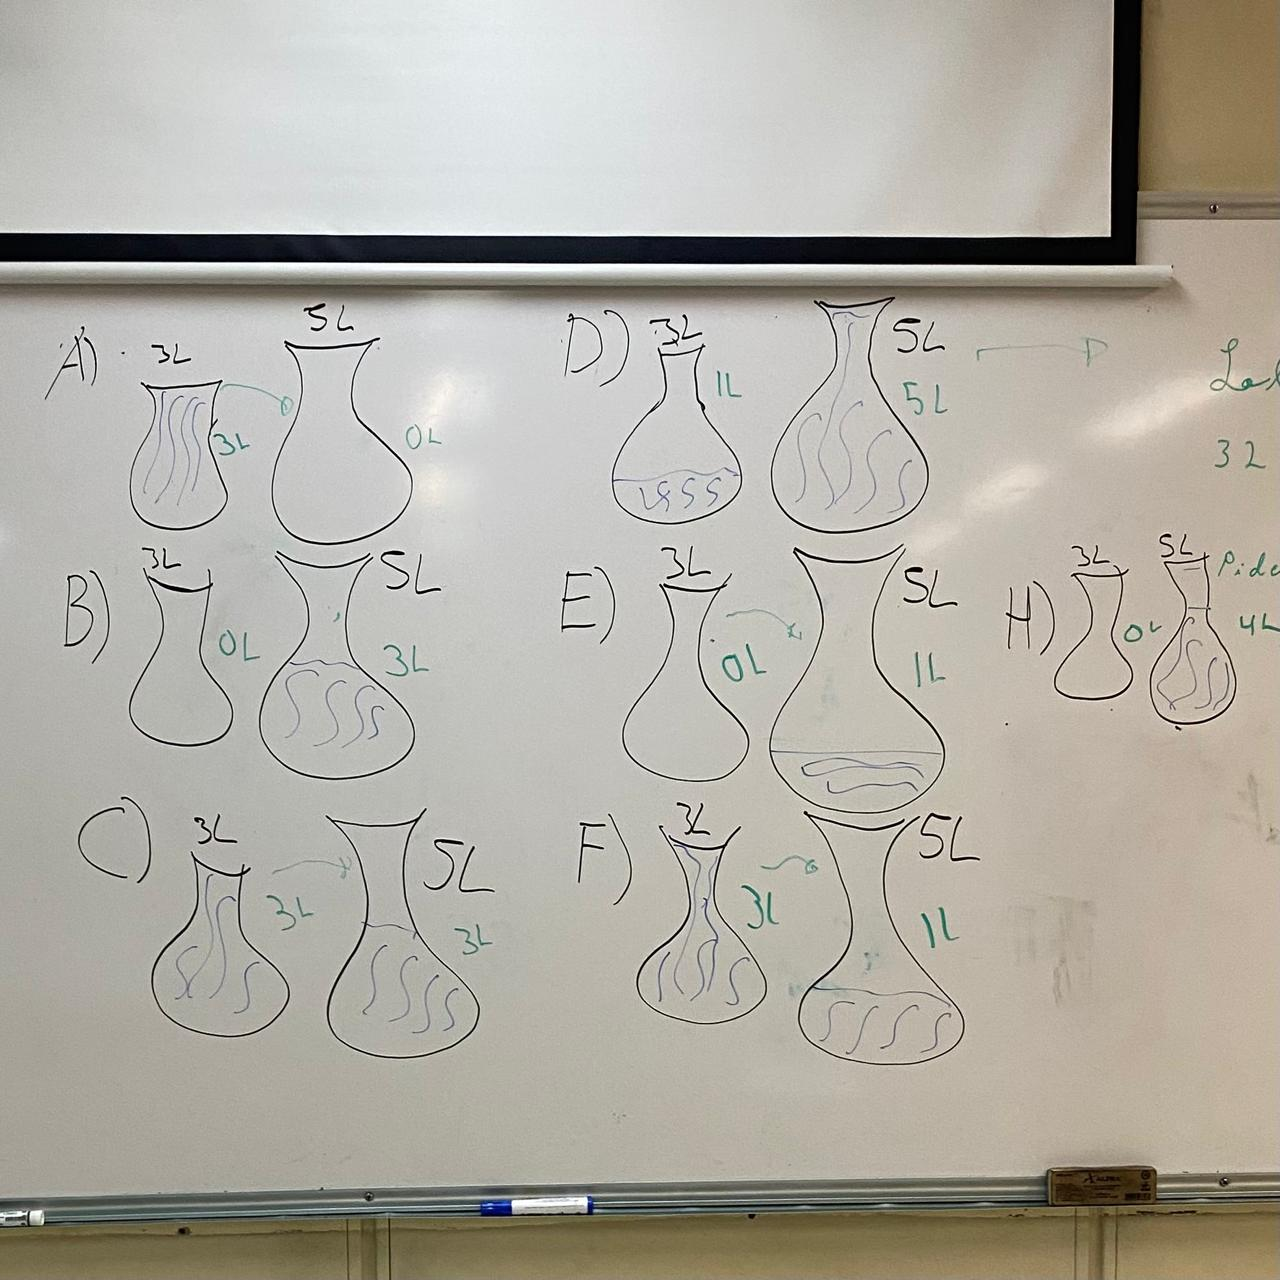
\includegraphics[scale=0.09]{clase4/problema4.2.jpeg}&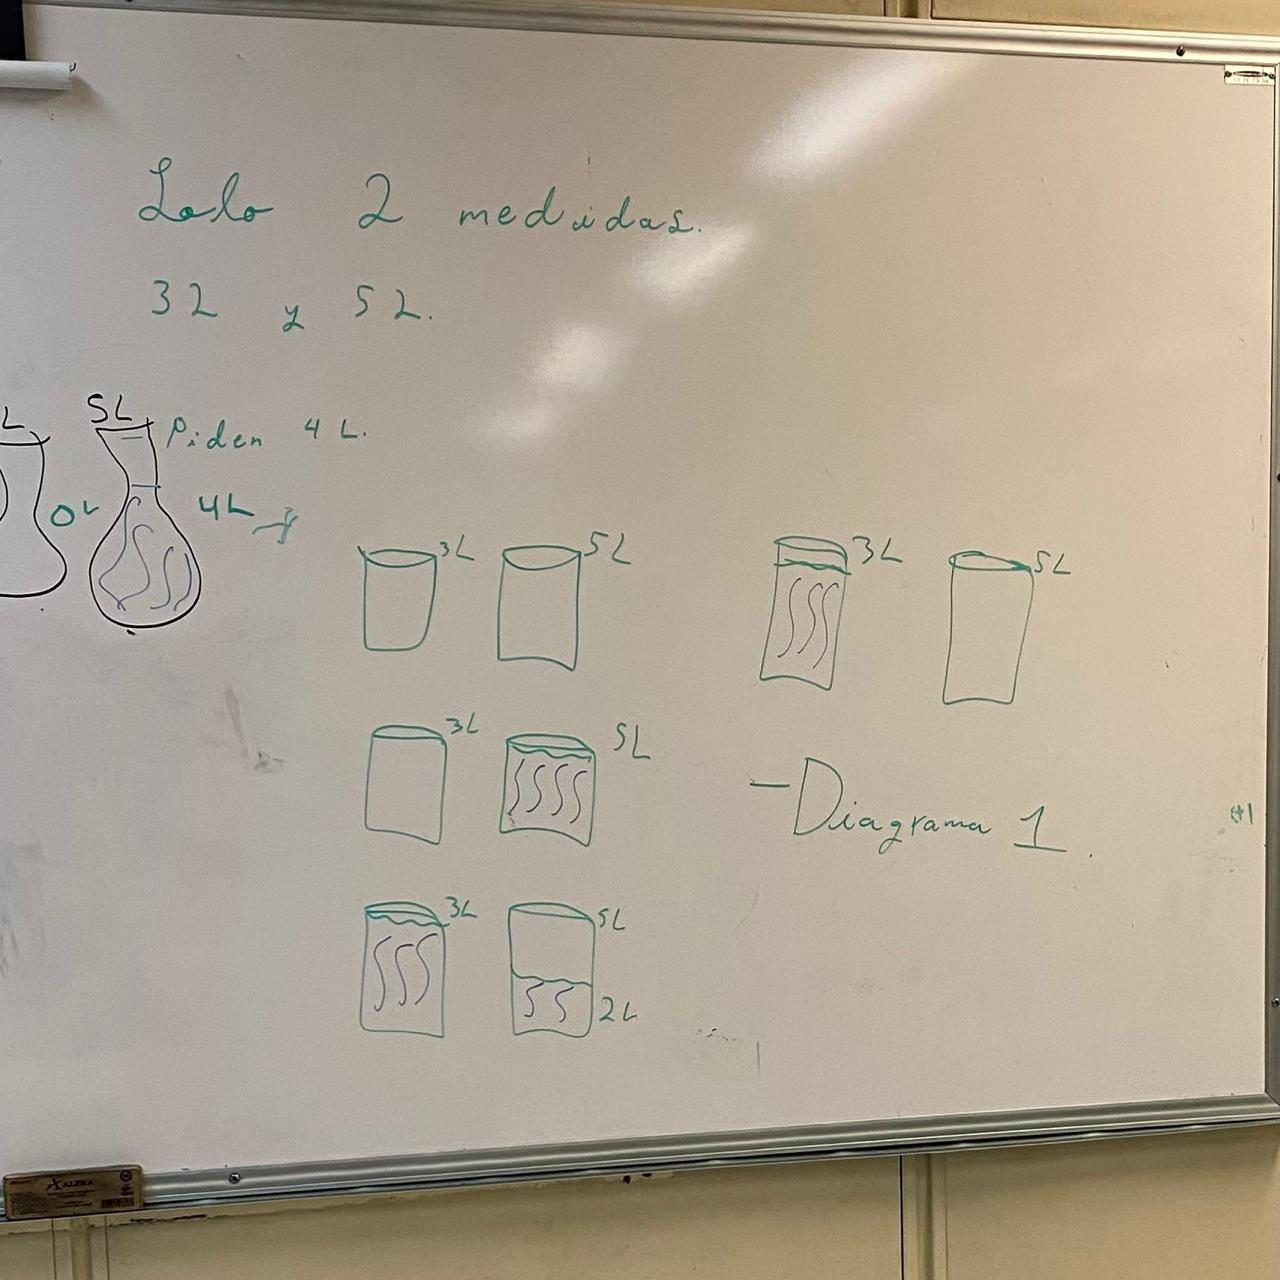
\includegraphics[scale=0.09]{clase4/problema4.3.jpeg}&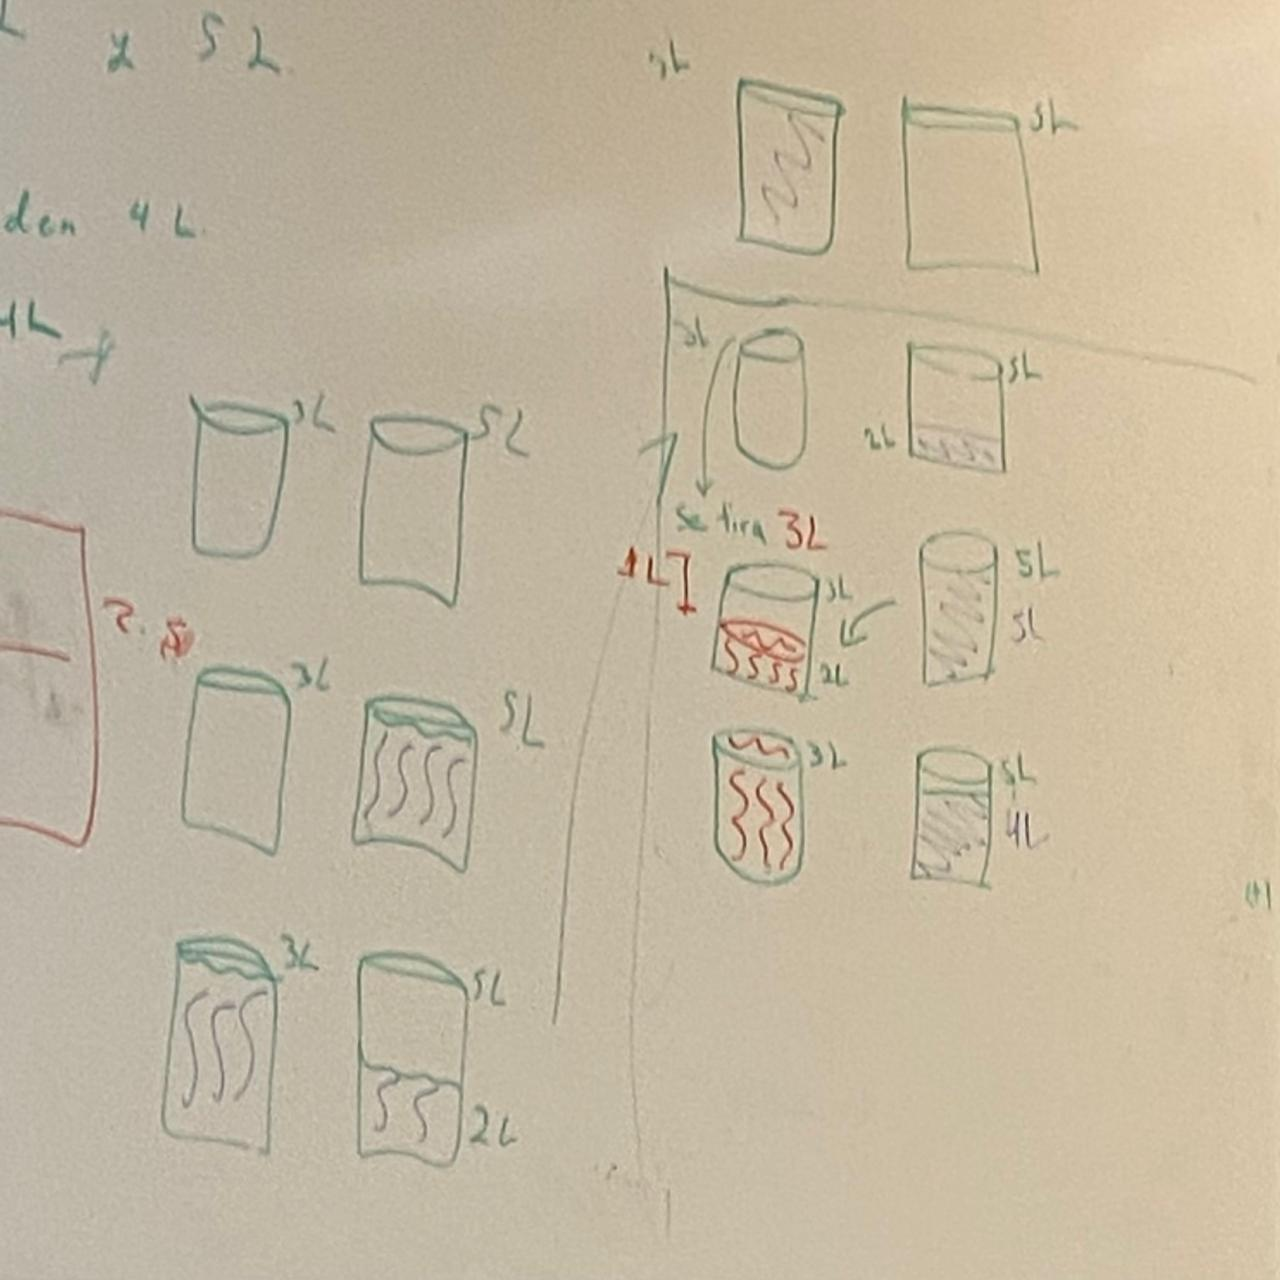
\includegraphics[scale=0.09]{clase4/problema4.4.jpeg}
        \end{tabular}
    \end{center}
\end{figure}

\section{Problema 5}
Fui parte del equipo que expuso la solución a este problema y se mencionaron las soluciones de la \hyperref[ejem:c3P5]{clase anterior}.

  %\chapter{Clase 5. Volumen de un prisma rectangular}\label{chap:C5}
\textbf{18/02/2025}

La clase comenzó con la realización de un trapecio rectangular por medio de origami y los pasos fueron los siguientes:
\begin{itemize}
    \item Doblar la hoja del punto $A$ al punto $Q$
    \item Doblar la hoja del punto $B$ al punto $P$
    \item Doblar la hoja del punto $D$ de al punto $P'$
    \item Doblar la hoja del punto $C$ al punto $Q'$
\end{itemize}

De modo que sobre la hoja queden las siguientes marcas:

\begin{figure}[h!]
    \caption{Representación de la hoja sobre la cual se trabajó}
    \begin{center}
        \begin{tikzpicture}
            % Dibujar el rectángulo (hoja)
            \draw[thick] (-3,5) -- (3,5) -- (3,-5) -- (-3,-5) --cycle;
            \node at (-3.2,5.2) {\textbf{$A$}};
            \node at (3.2,5.2) {\textbf{$B$}};
            \node at (3.2,-5.2) {\textbf{$C$}};
            \node at (-3.2,-5.2) {\textbf{$D$}};
            
            \draw[thin] (3,-5) -- (-3,2);
            \node at(-3.2,2.2){\textbf{$P$}};
            \draw[thin] (3,2) -- (-3,-5);
            \node at(3.2,2.2){\textbf{$Q$}};
            
            \draw[thin] (3,-2) -- (-3,5);
            \node at(-3.2,-2.2){\textbf{$P'$}};
            \draw[thin] (3,5) -- (-3,-2);
            \node at(3.2,-2.2){\textbf{$Q'$}};
        \end{tikzpicture}
    \end{center}
\end{figure}

Luego deben unirse los siguientes puntos: 

\begin{itemize}
    \item $A$ y $B$
    \item $C$ y $D$
    \item $P'$ y $P$
    \item $Q'$ y $Q$
\end{itemize}
Y hacer los dobleces de la hoja hacia adentro de modo que quede algo similar a esto:

\begin{center}
    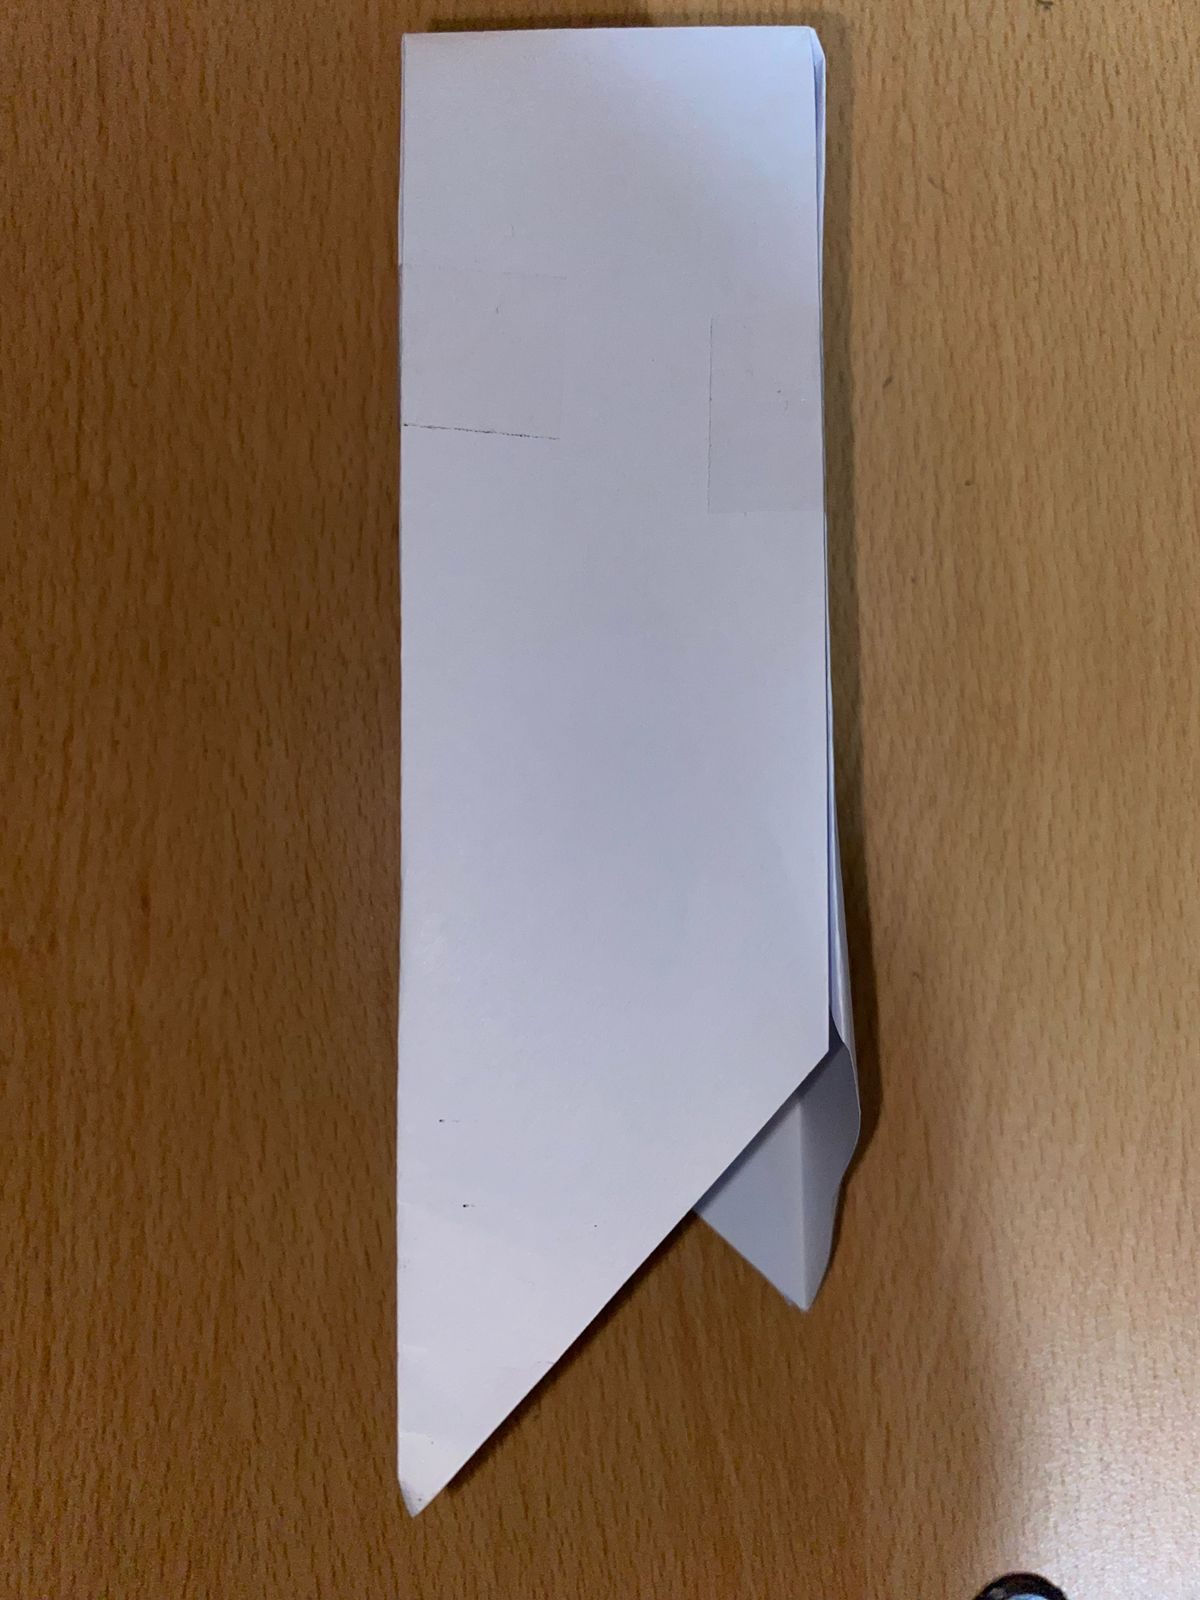
\includegraphics[scale=0.1]{clase5/semiTrapecio.jpeg}
\end{center}

Despues se doblan las puntas, de modo que quede el prisma de la siguiente forma.

\begin{center}
    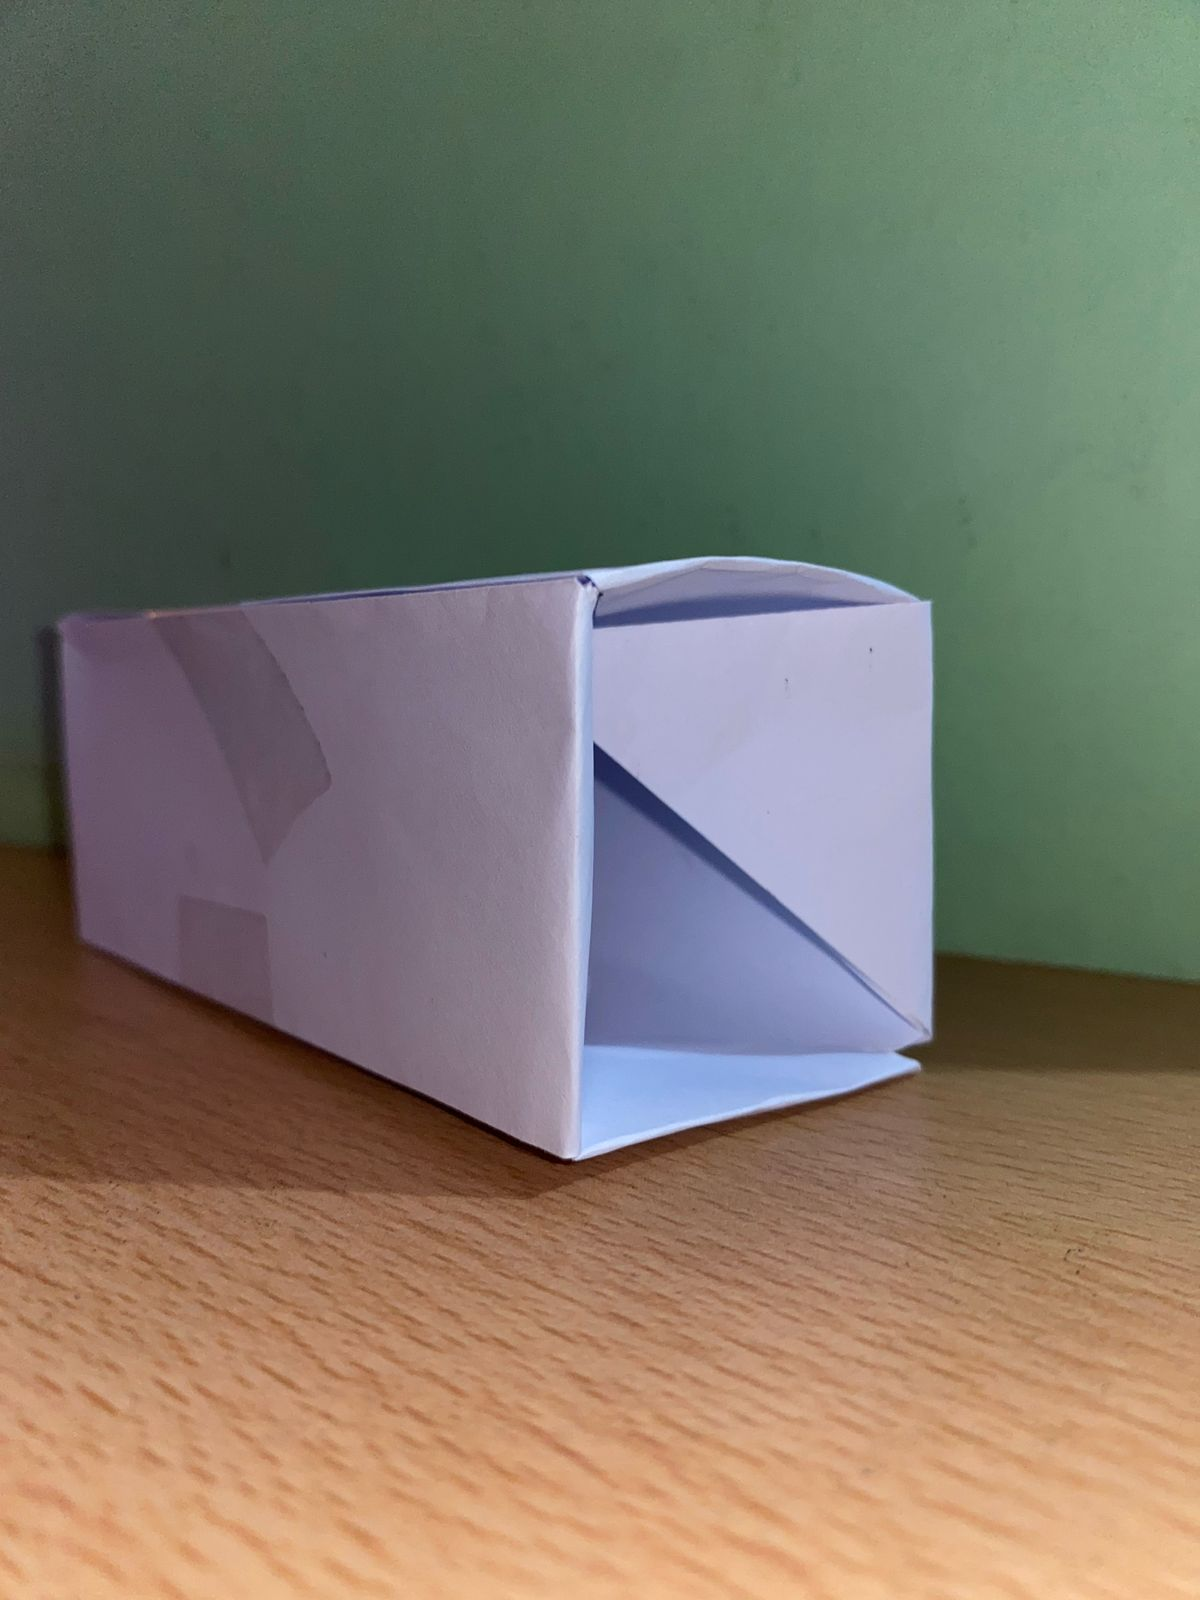
\includegraphics[scale=0.09]{clase5/trapecioFin.jpeg}
\end{center}

Y se hace uno similar para un cuarto del tamaño de la hoja
\begin{figure}[ht!]
    \begin{center}
        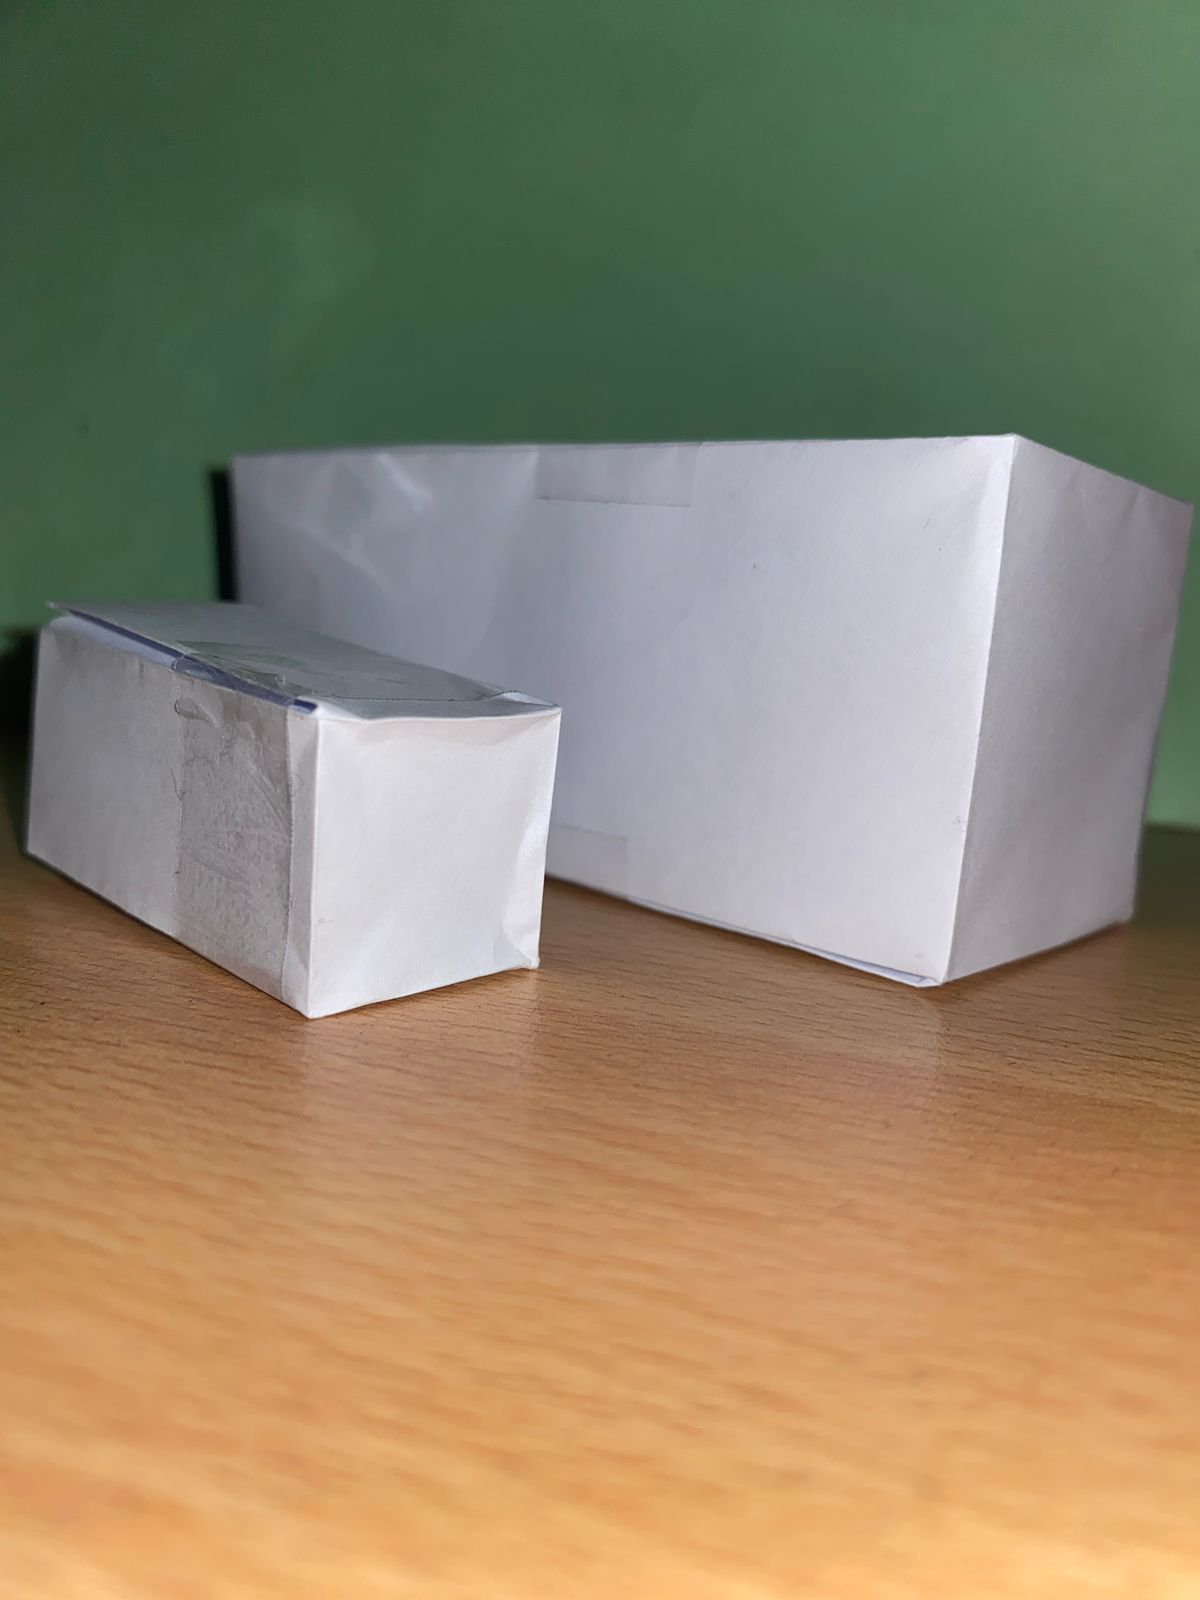
\includegraphics[scale=0.09]{clase5/prismaPyG.jpeg}
    \end{center}
\end{figure}

Durante la actividad la primera pregunta fue ¿Cuántos prismas pequeños caben en el prisma grande? Nuestra respuesta como equipo fue 4, pero luego sacando el volumen del prisma grande y de un prisma pequeño, nos dimos cuenta de que cabían 8

\textbf{¿Cómo encontramos la fórmula para el volumen de un prisma pequeño?}

Primero medimos la altura de los prismas y buscamos encontrar alguna proporción, la cual fue de $\frac{1}{2}$ de cualquiera de las medidas del prisma grande al prisma pequeño y posterior a eso surgió la idea ilustrada abajo. 

\begin{figure}[ht!]
    \begin{center}
        \begin{tikzpicture}
            % Proporciones normales
            \draw[thick] (-5,5) -- (-2,5) -- (-2,0) -- (-5,0) --cycle;
            \draw[<->] (-5,-0.5) -- (-2,-0.5);
            \node at (-3.5,-0.8) {\textbf{$x$}};
            \draw[<->] (-1.5,0) -- (-1.5,5);
            \node at (-1,2.5) {\textbf{$y$}};
            
            % Proporciones reducidas
            \draw[thick] (0,5) -- (3,5) -- (3,0) -- (0,0) --cycle;
            % Dividiendo la hoja en 4 partes
            \draw[dashed] (1.5,5) -- (1.5,0);
            \draw[dashed] (0,2.5) -- (3,2.5);
            % Flechas reducidas
            \draw[<->] (1.5,-0.5) -- (3,-0.5);
            \node at (2.4,-0.8) {\textbf{$\frac{x}{2}$}};
            \draw[<->] (3.5,0) -- (3.5,2.5);
            \node at (3.8,1.5) {\textbf{$\frac{y}{2}$}};
        \end{tikzpicture}
    \end{center}
    \caption{Aunque el material usado se redujo a un cuarto, la medida del largo y del ancho solo se redujeron a la mitad}
\end{figure}

Después de esto solo trabajamos sobre la fórmula para calcular el volumen de un prisma rectangular:

\begin{gather*}
    f(x) =  V_G \\
    V_G = lah \qquad \text{Donde $l$: largo, $a$: ancho y $h$: altura } \\
    V_p = \frac{l}{2} \cdot \frac{a}{2} \cdot \frac{h}{2}\\
    V_p = \frac{lah}{8}\\
    V_p = \frac{V_G}{8}\\
    V_p \cdot 8= V_G
\end{gather*}

  %\section{Clase 6. Exposición}
\textbf{25/02/2025}

Cada equipo expuso una solución al problema planteado la clase anterior, el cual era hallar una fórmula para calcular el volumen del prisma grande, y así obtener cuantos prismas pequeños cabían.

\section{Solución 1}
Uno de los equipos expuso de manera geométrica la relación que guardaba cada dobles en la realización de los prismas. Lo que hicieron fue triangular la hoja y observaron qué relación de proporcionalidad se conservaba a medida que se realizaban dobleces en la hoja, aunque en ningún momento llegaron a la solución para conocer la cantidad de prismas pequeños que caben en el prisma grande

\begin{center}
    \begin{figure}[H]
        \begin{tabular}{ccc}    
            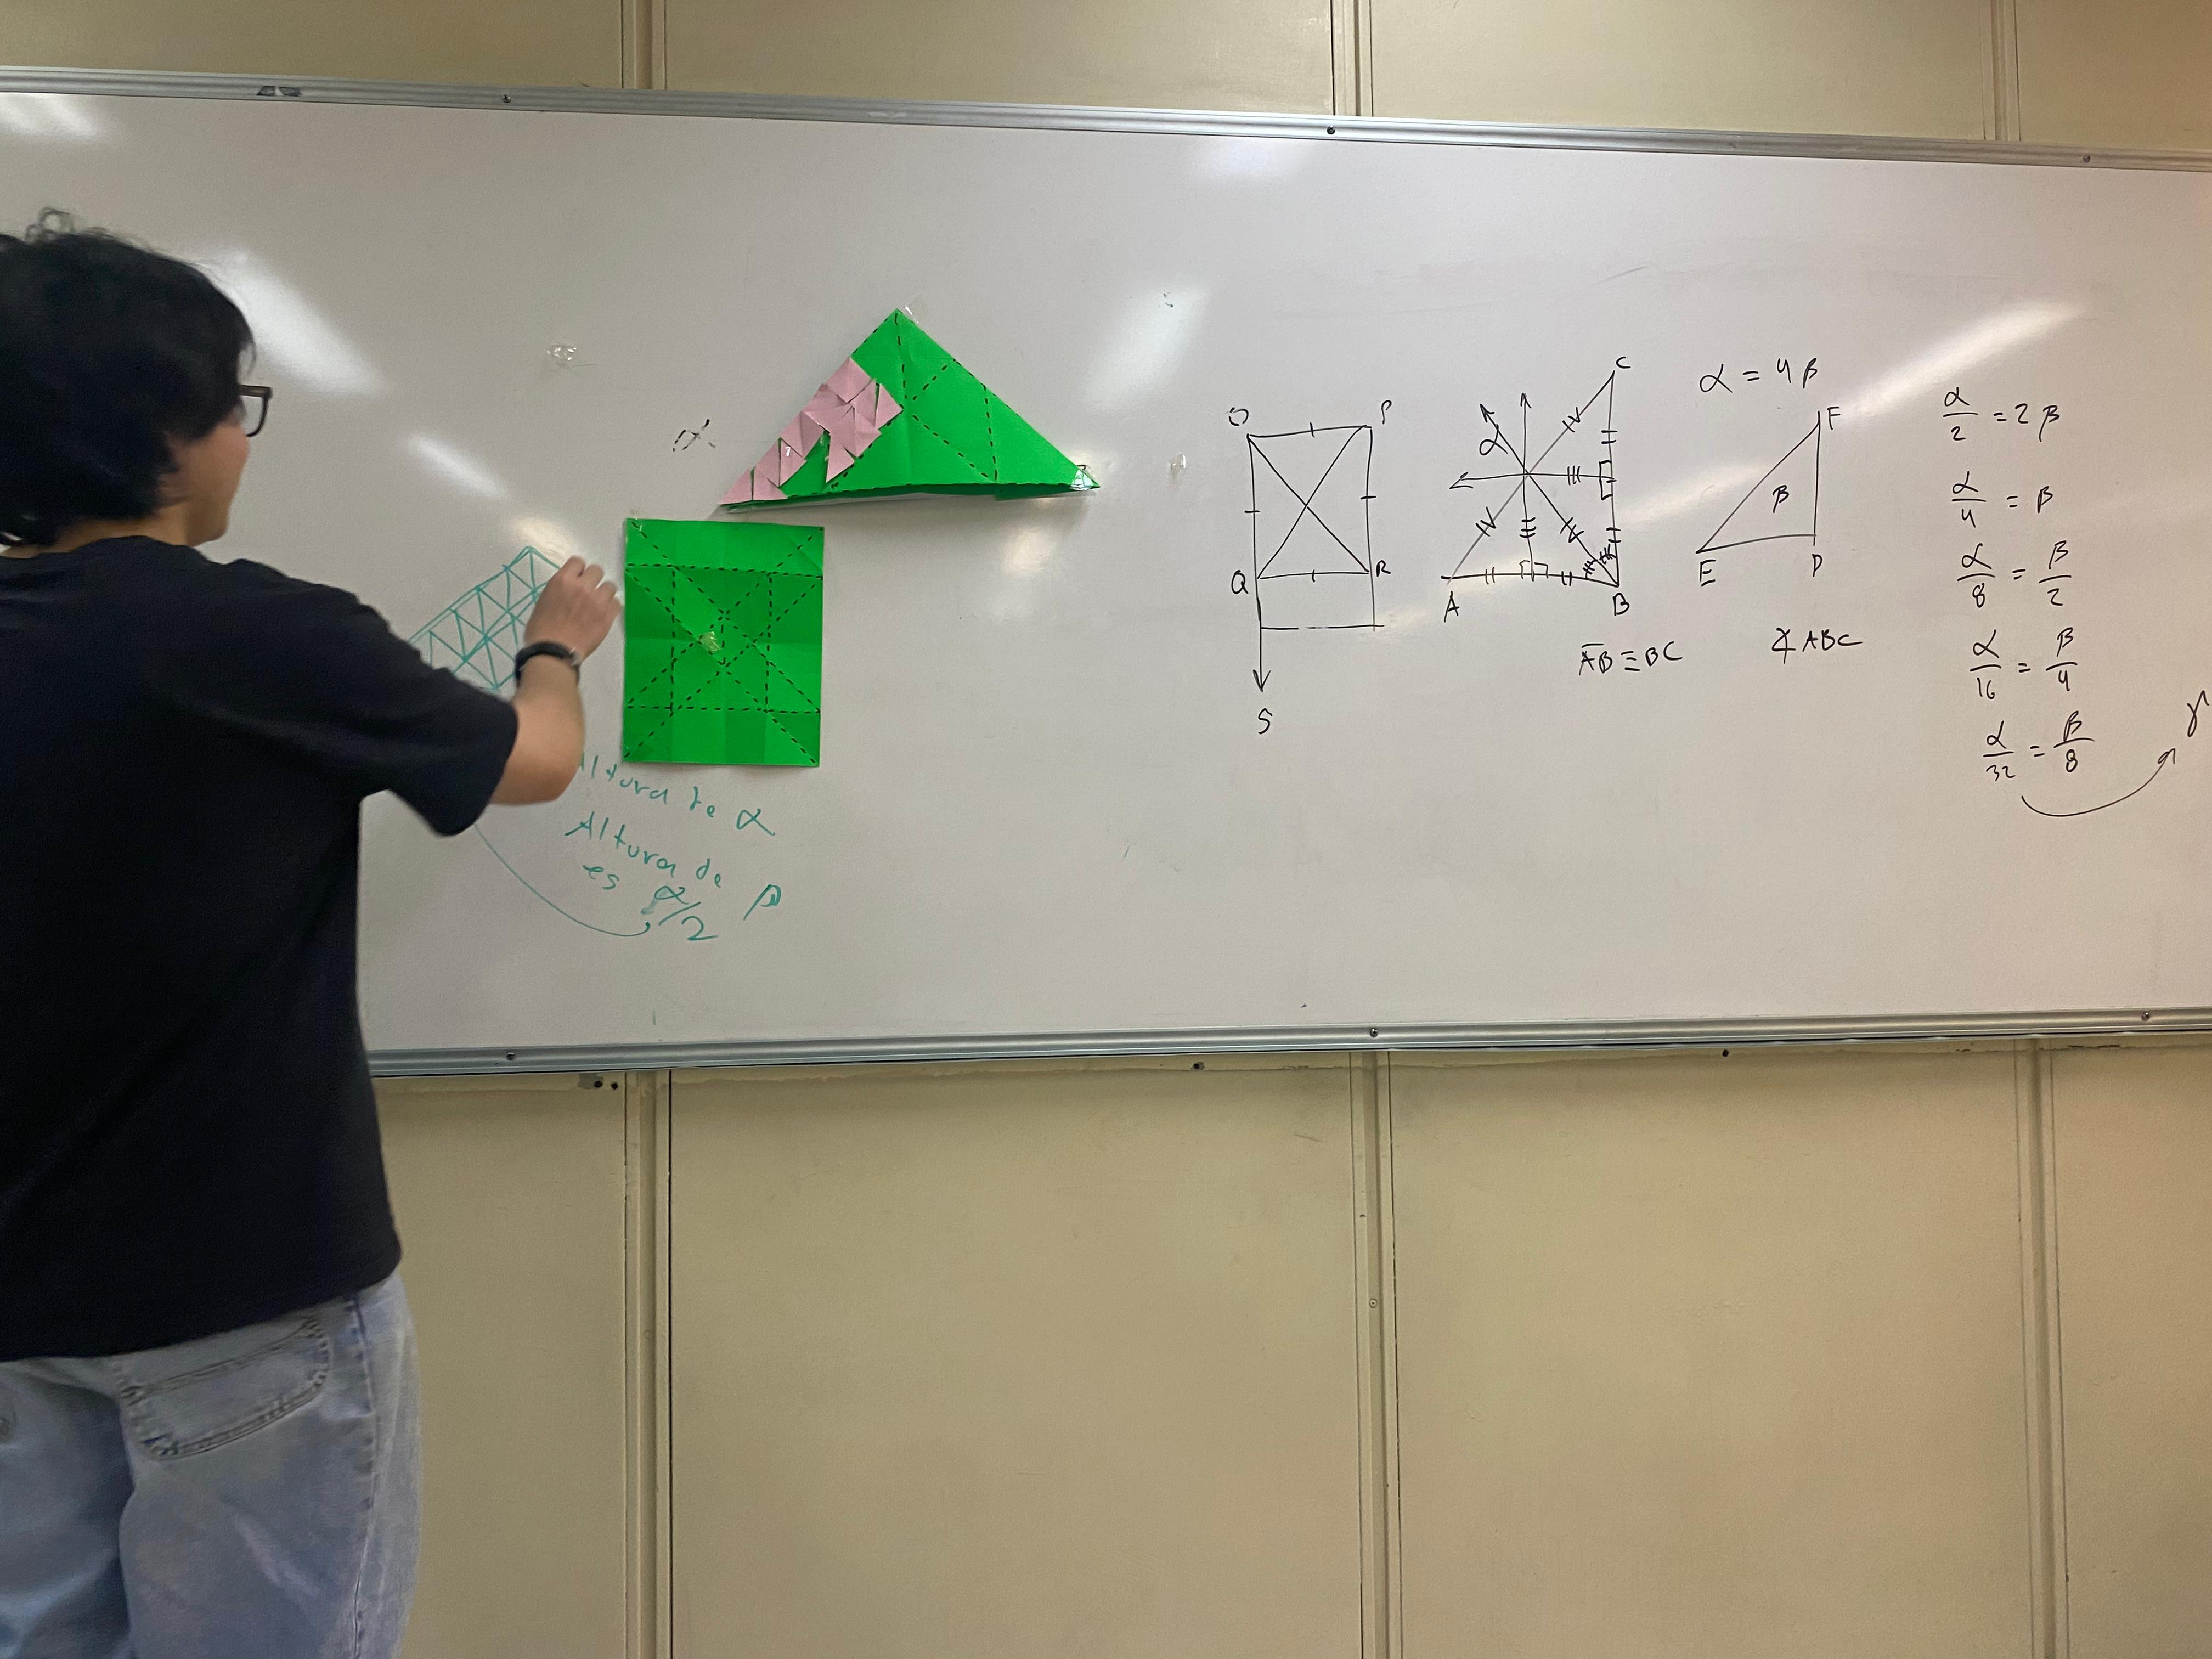
\includegraphics[scale = 0.05]{clase6/Equipo1-1.jpeg}&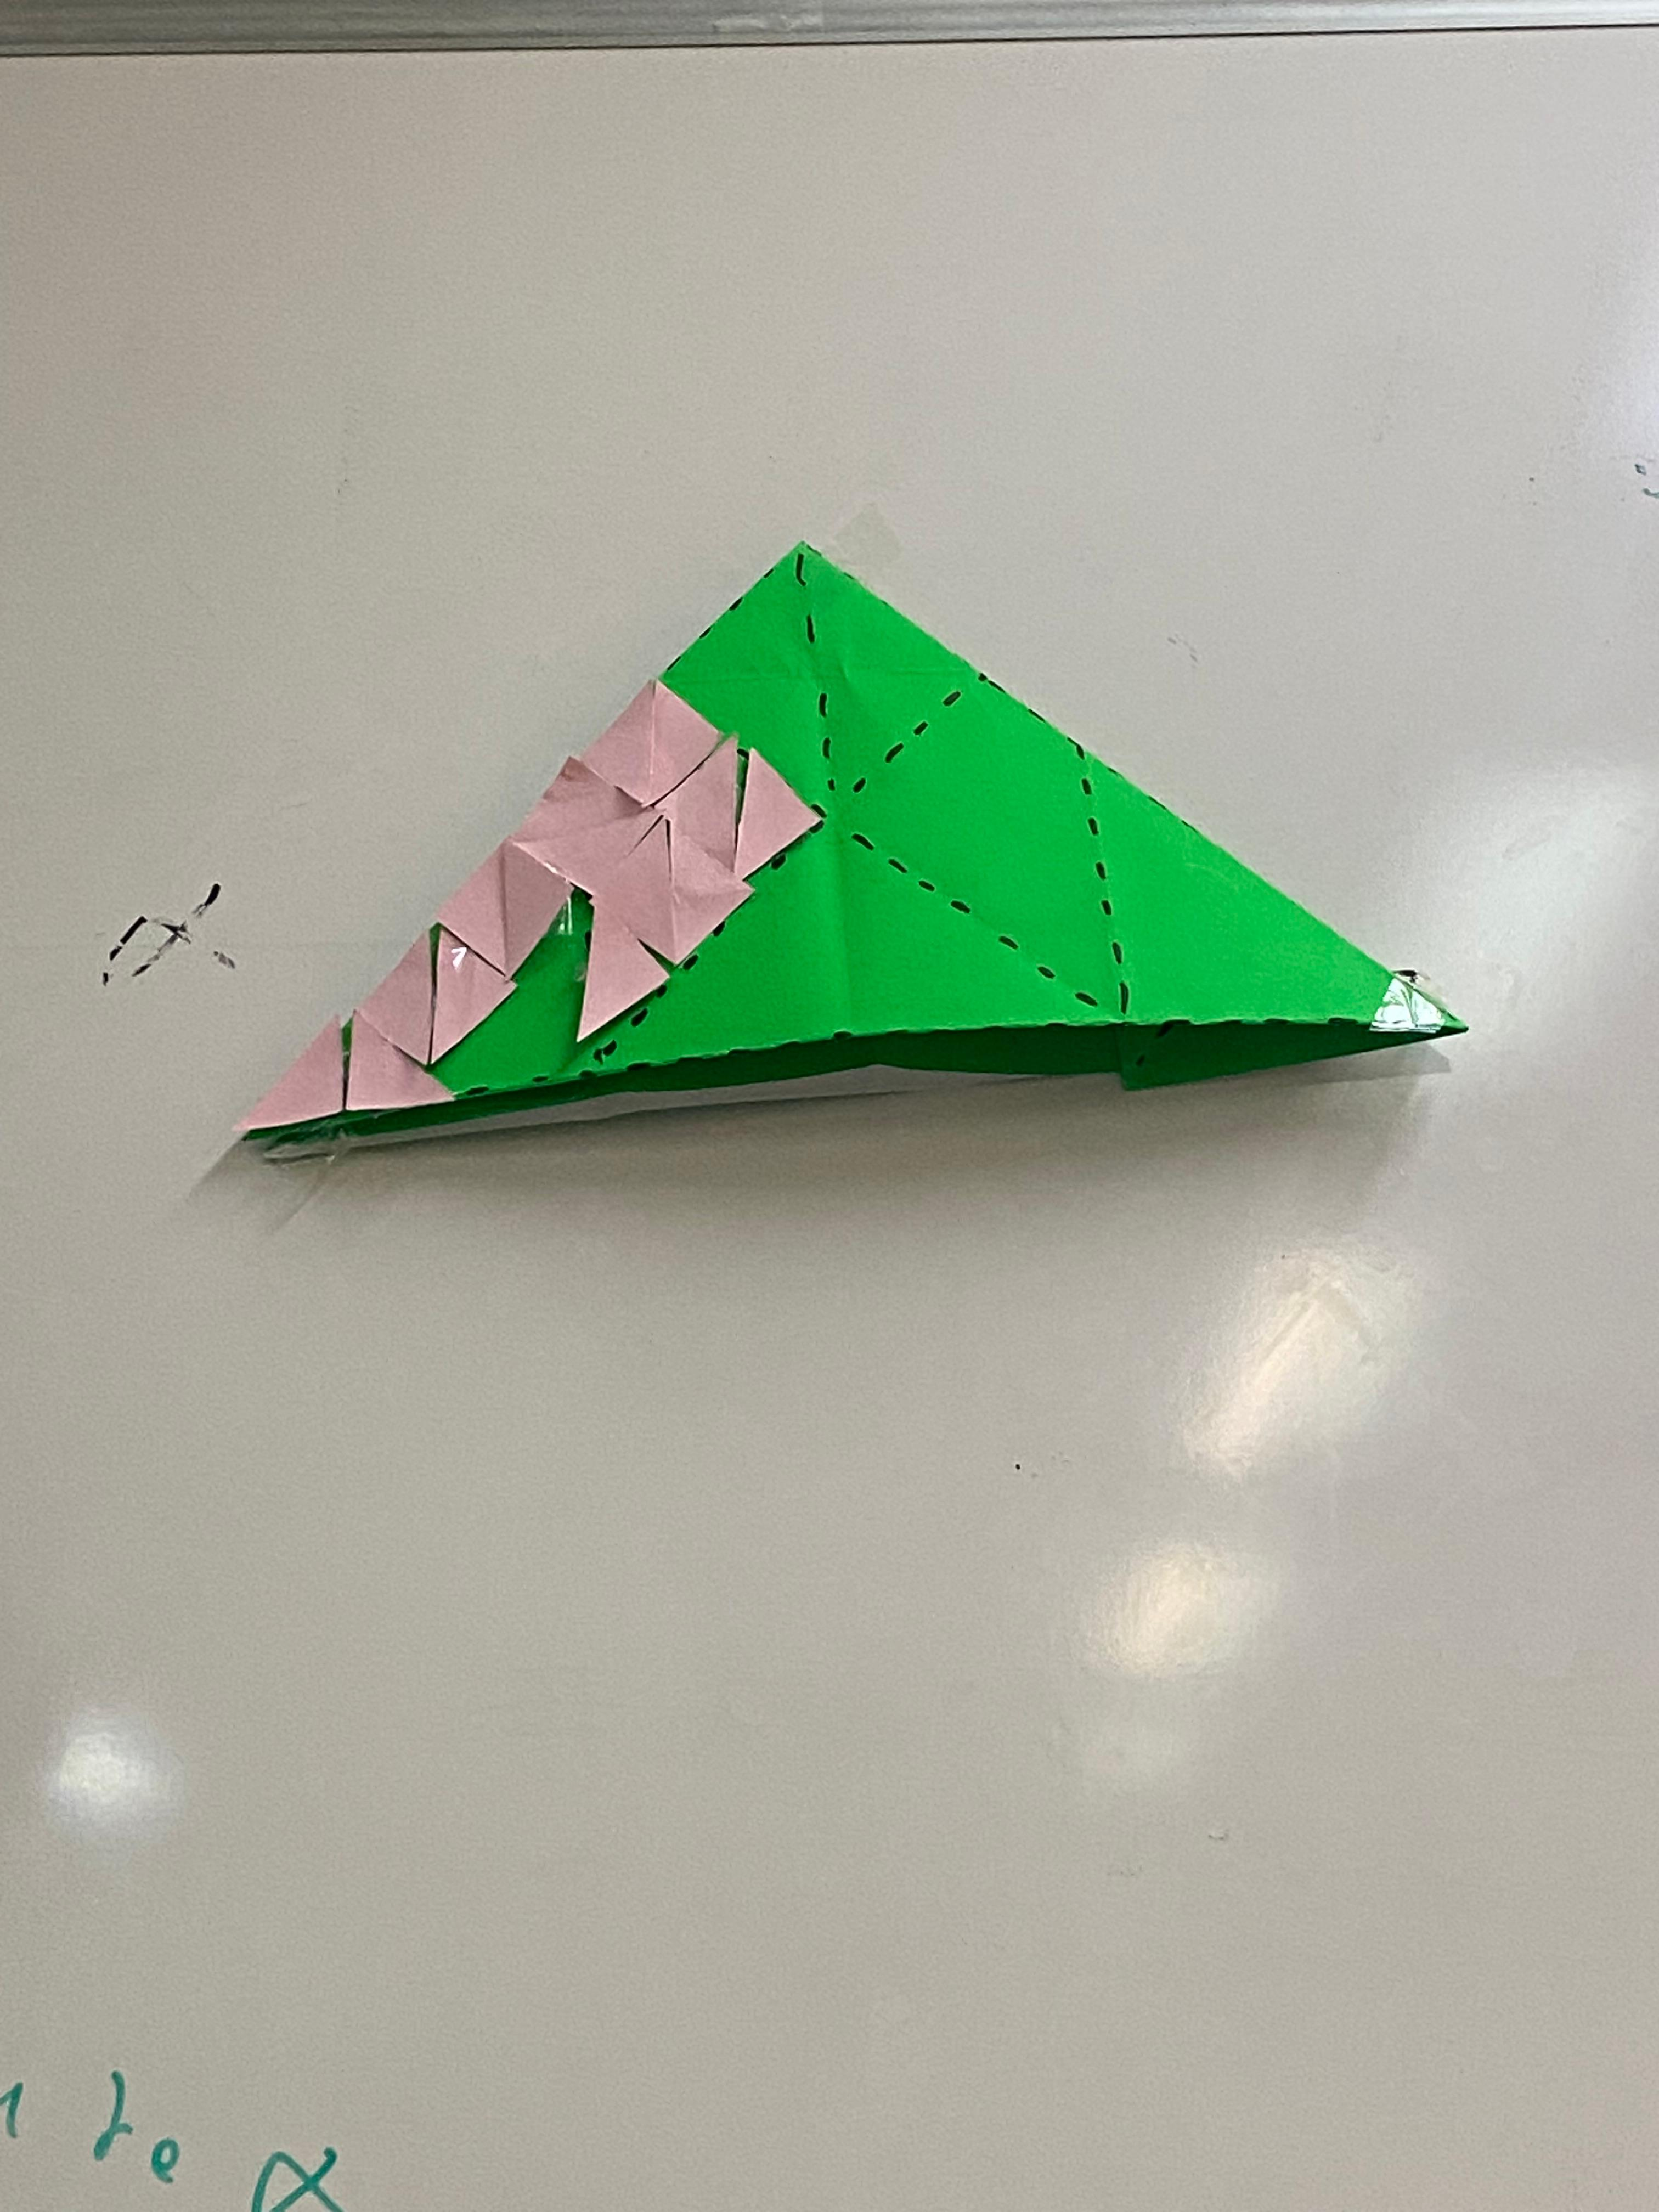
\includegraphics[scale = 0.04]{clase6/Equipo1-2.jpeg}&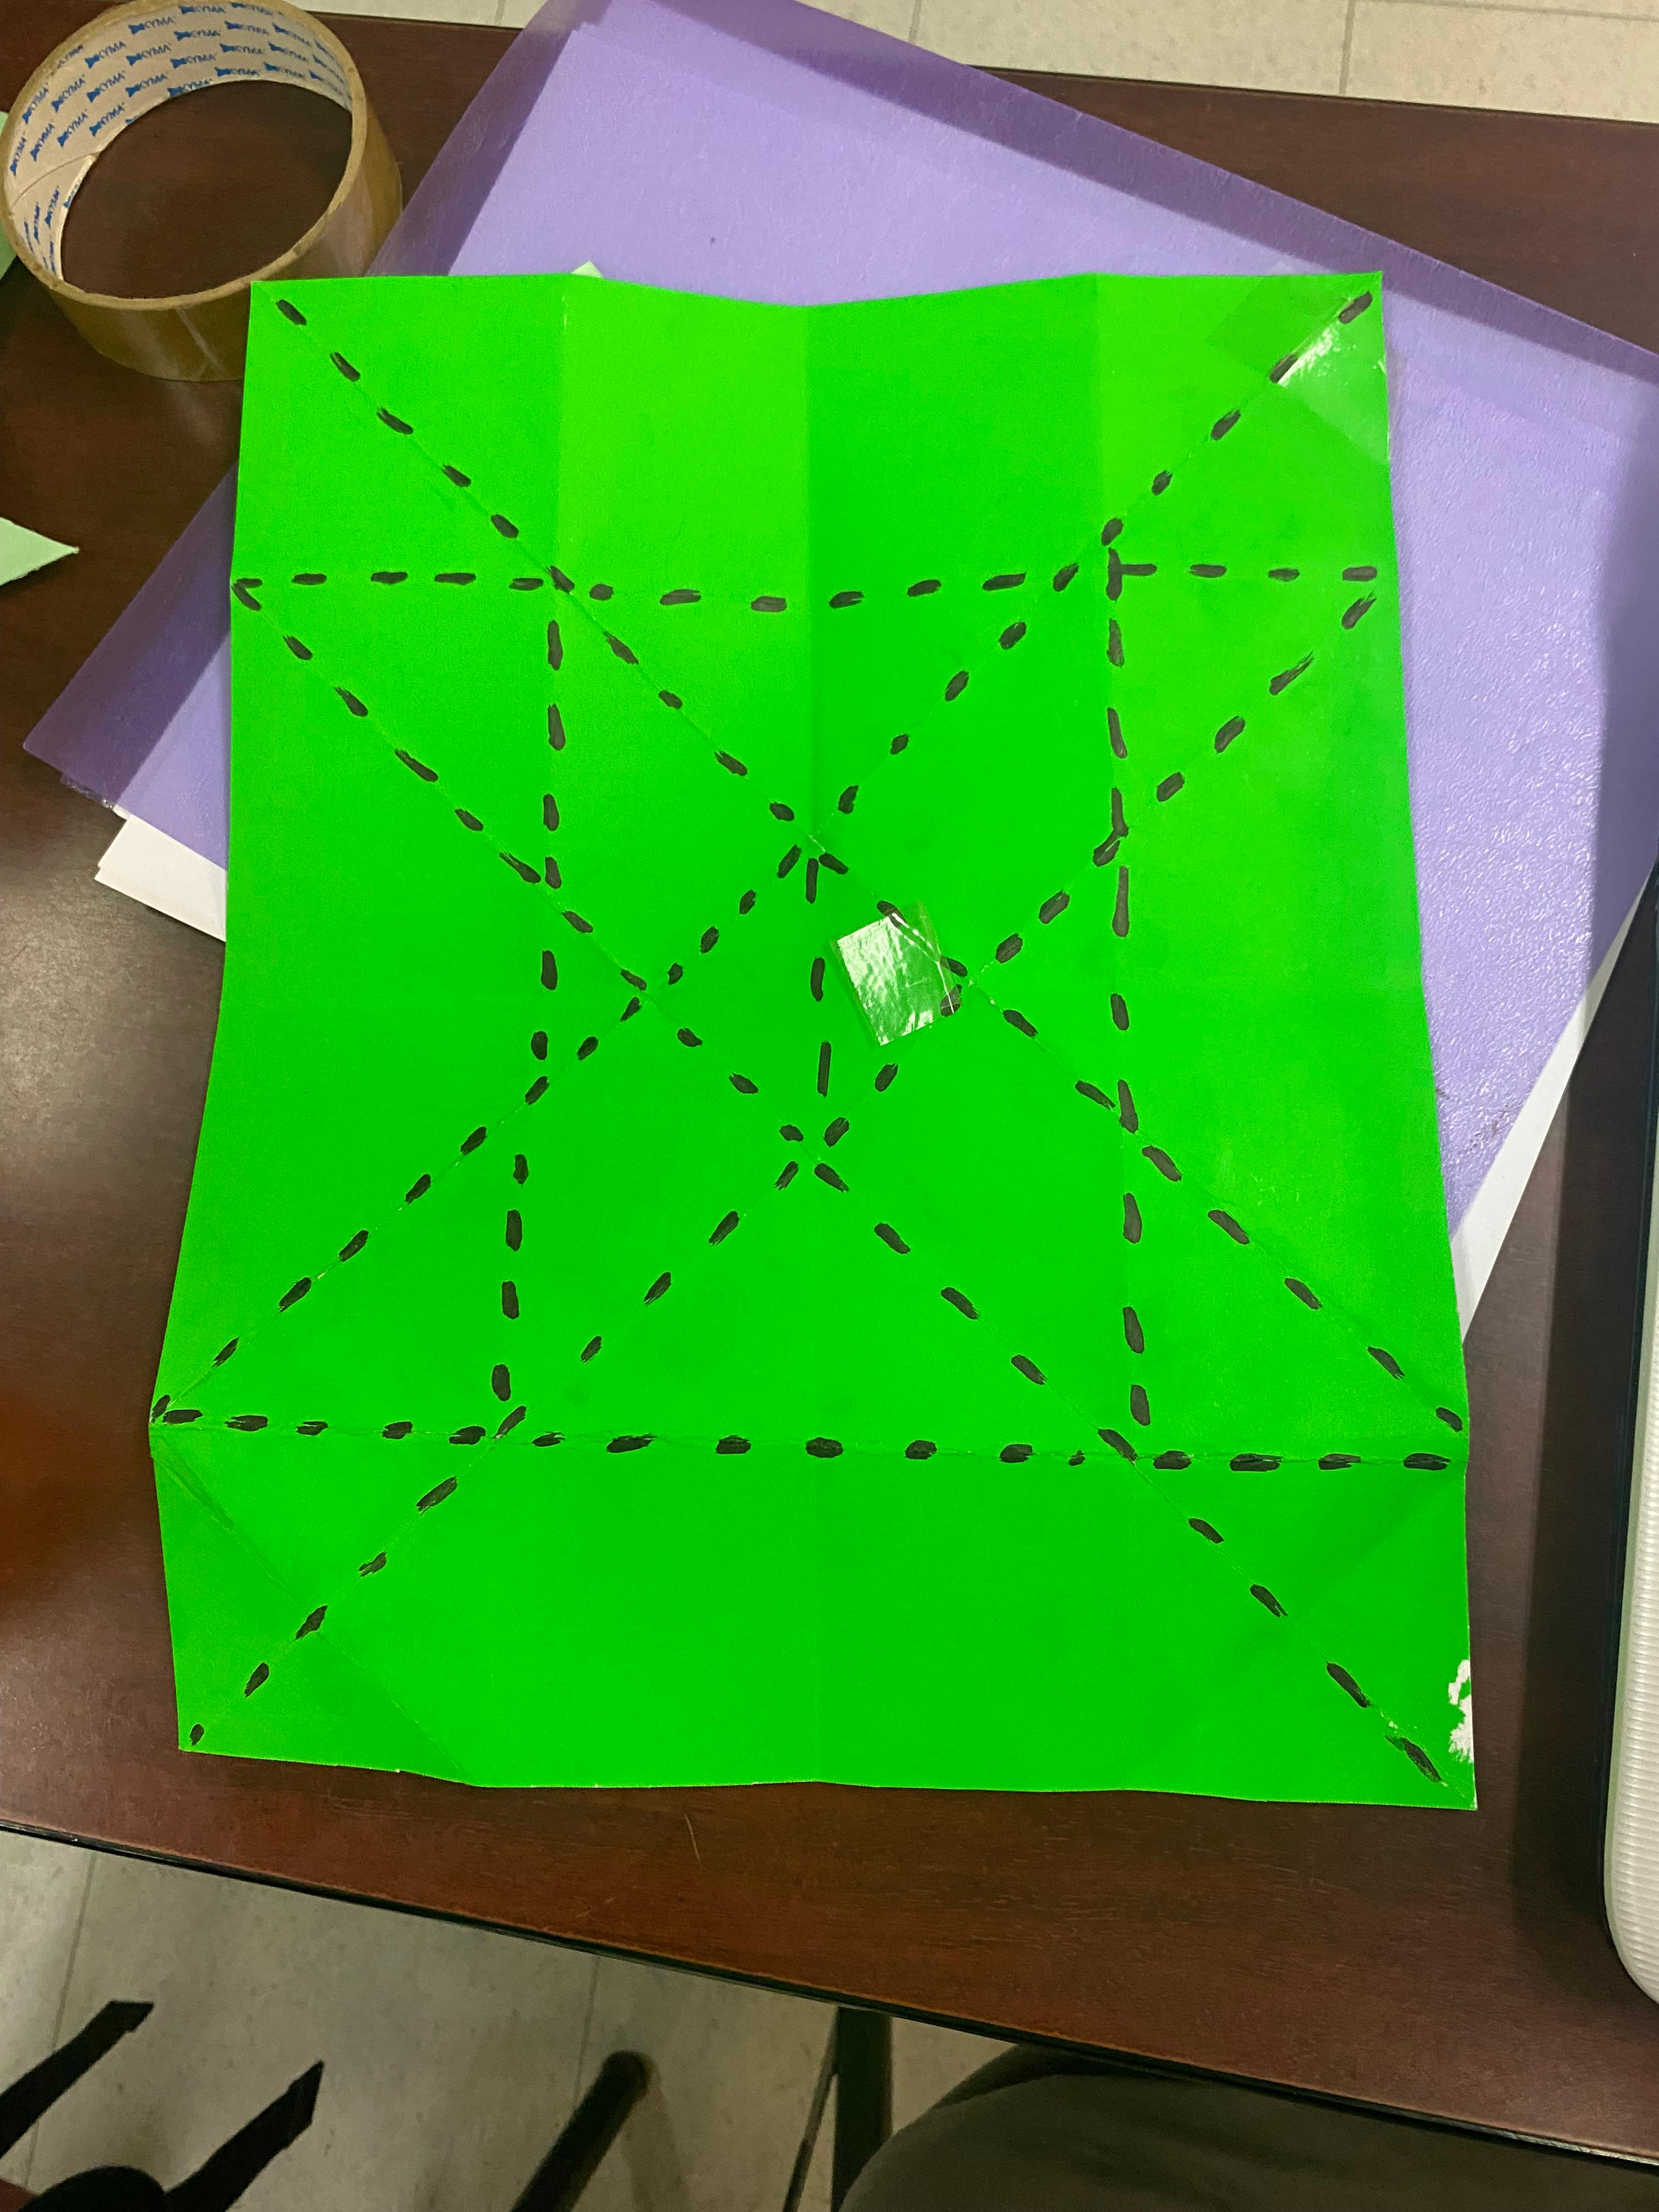
\includegraphics[scale = 0.04]{clase6/Equipo1-3.jpeg}
        \end{tabular}
        \caption{Desarrollo de la solución del equipo 1}
    \end{figure}
\end{center}

\section{Solución 2}

Los equipos restantes y mi equipo tuvimos una idea similar al momento de demostrar de donde obtuvimos la fórmula para calcular el volumen, la cual fue observando que la hoja al momento de ser dividida en cuatro partes, las dimensiones de largo y alto se partían a a la mitad, y aunque no podemos demostrar explícitamente como de una figura en dos dimensiones la medida que nos da la tercera dimensión. Guarda la misma relación. Nuestro argumento fue que al salir el cuerpo geométrico de una figura geométrica (de 2D a 3D), la tercera dimensión iba a guardar la misma relación que las otras dos; consulte \hyperref[chap:C5]{el capitulo anterior para ver el procedimiento que siguió mi equipo.}

\begin{figure}[H]
    \centering %Centra horizontalmente
    \begin{tabular}{cc}
        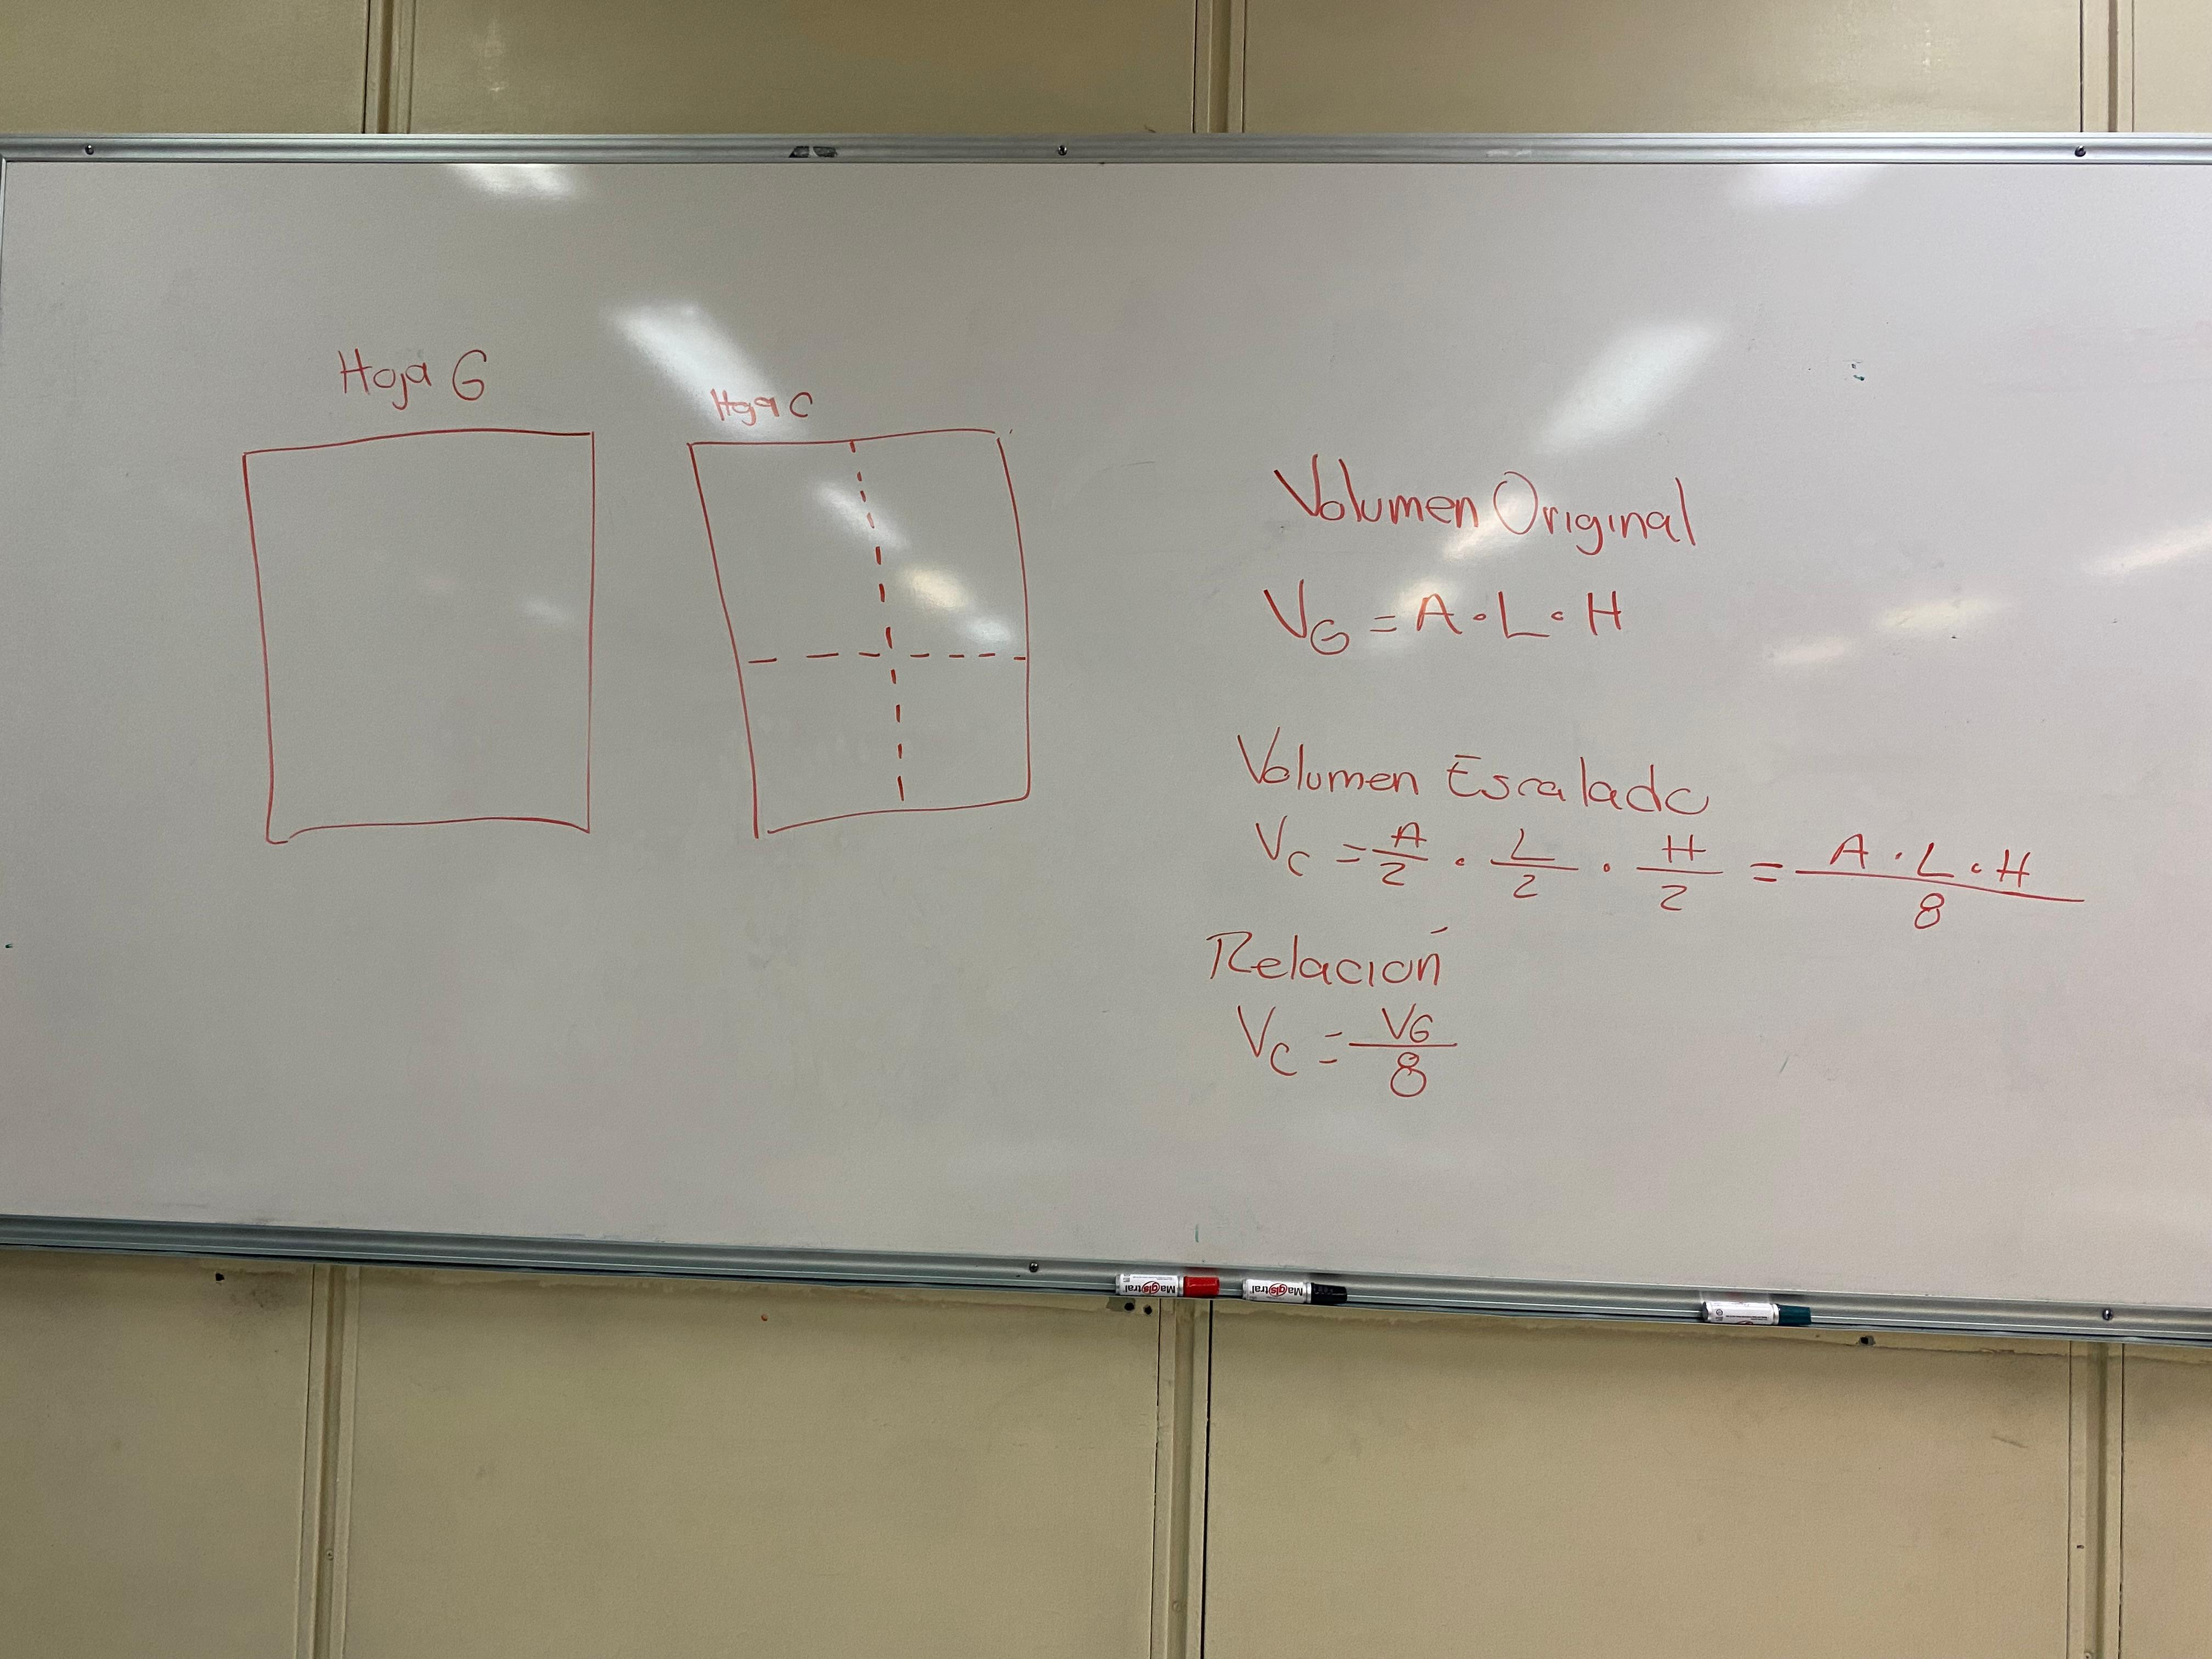
\includegraphics[scale=0.045]{clase6/Equipo2.jpeg}&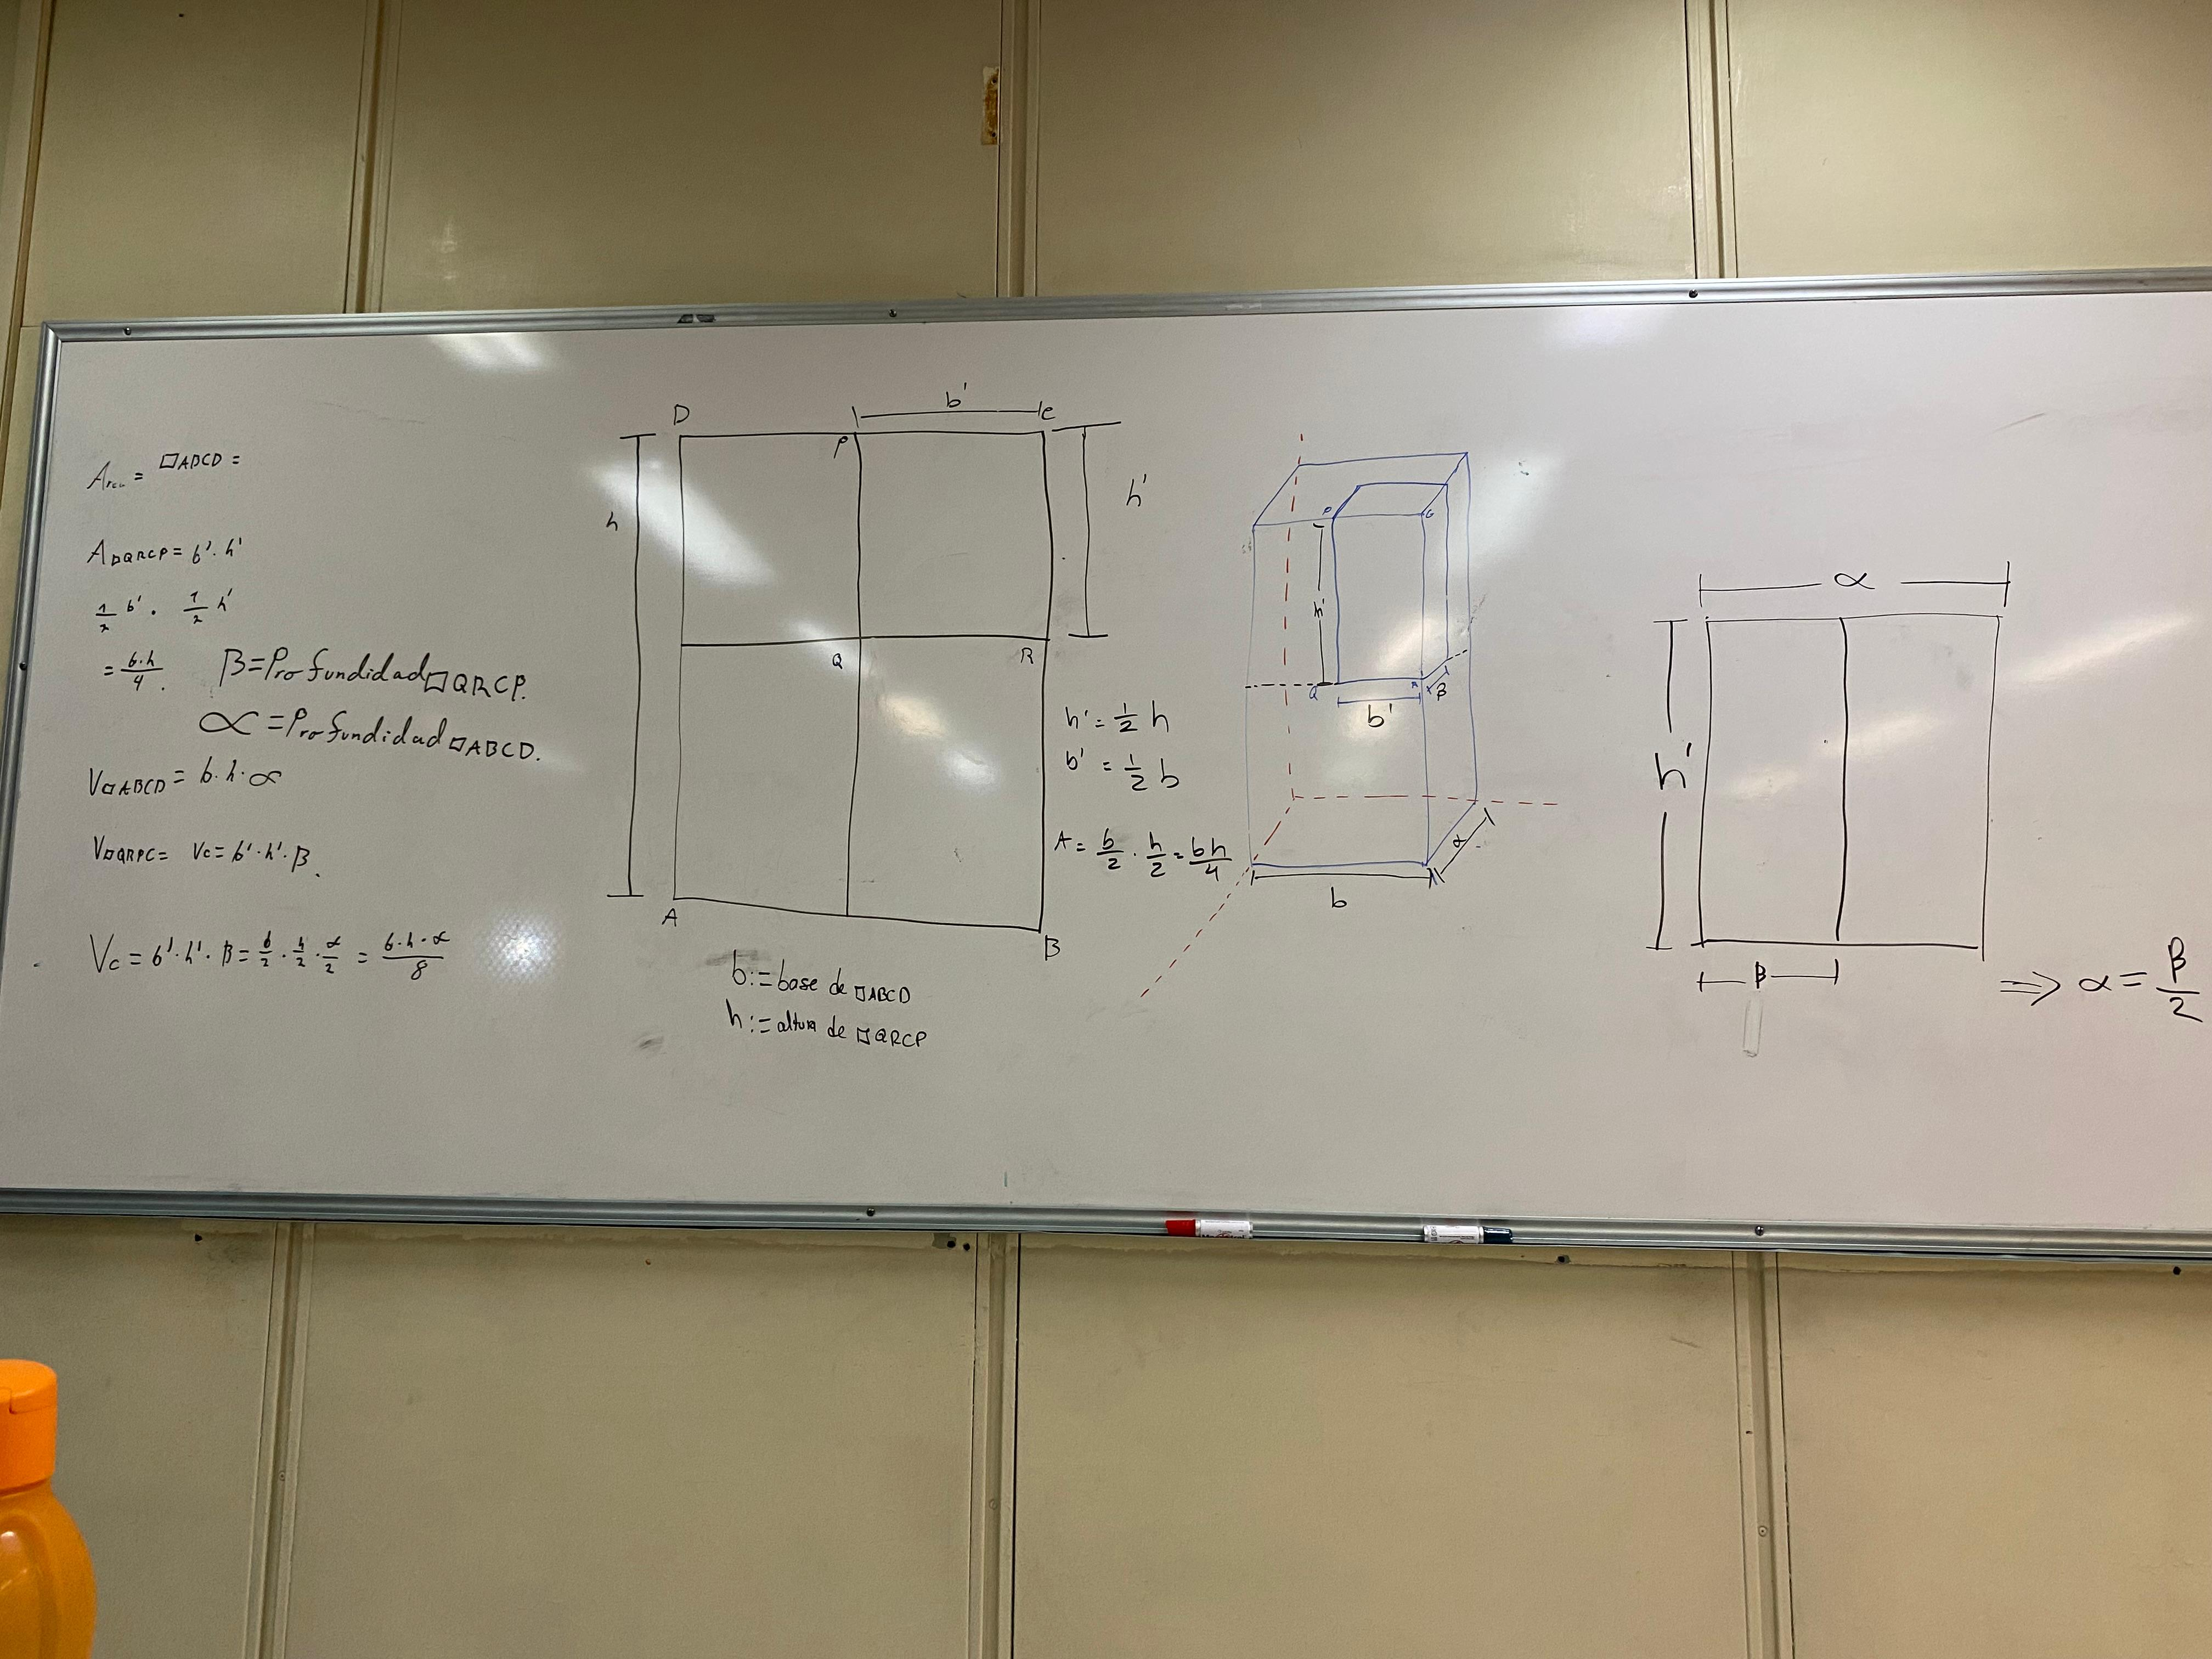
\includegraphics[scale=0.045]{clase6/Equipo3.jpeg}
    \end{tabular}
    \caption{Soluciones similares de los equipos 2, 3 y 4}
\end{figure}
  %\section{Clase 7. Rompecabezas}
\textbf{26/02/2025}

Durante la clase resolvimos varios rompecabezas haciendo uso del pensamiento lateral, y de igual modo con ciertas habilidades como la motricidad fina. 

La idea de la clase era tomar 10 minutos para resolver cada rompecabezas y al momento de completarlo intercambiar con otro compañero que ya hubiese terminado de resolver alguno, y si durante esos 10 minutos no habíamos podido resolverlo, podíamos recurrir a ciertos folletos que tenían pistas o explícitamente las soluciones. 

\section{Rompecabezas 1. Hextricks}

En mi caso, el primer rompecabezas que agarré fue el Hextricks el cual, ni aún teniendo el folleto, puede resolver exitosamente; la cuestión, por la cual me fue difícil armarlo, es mi falta de desarrollo de la motricidad fina, pues ciertas piezas no las podía unir. Durante los primeros 50 minutos lo hice de manera individual y después un compañero comenzó a ayudarme y aún así no lo logramos.

\begin{figure}[H]
    \begin{tabular}{cc}
        Hextricks antes de ser desarmado & Proceso fallido de armado\\\\
        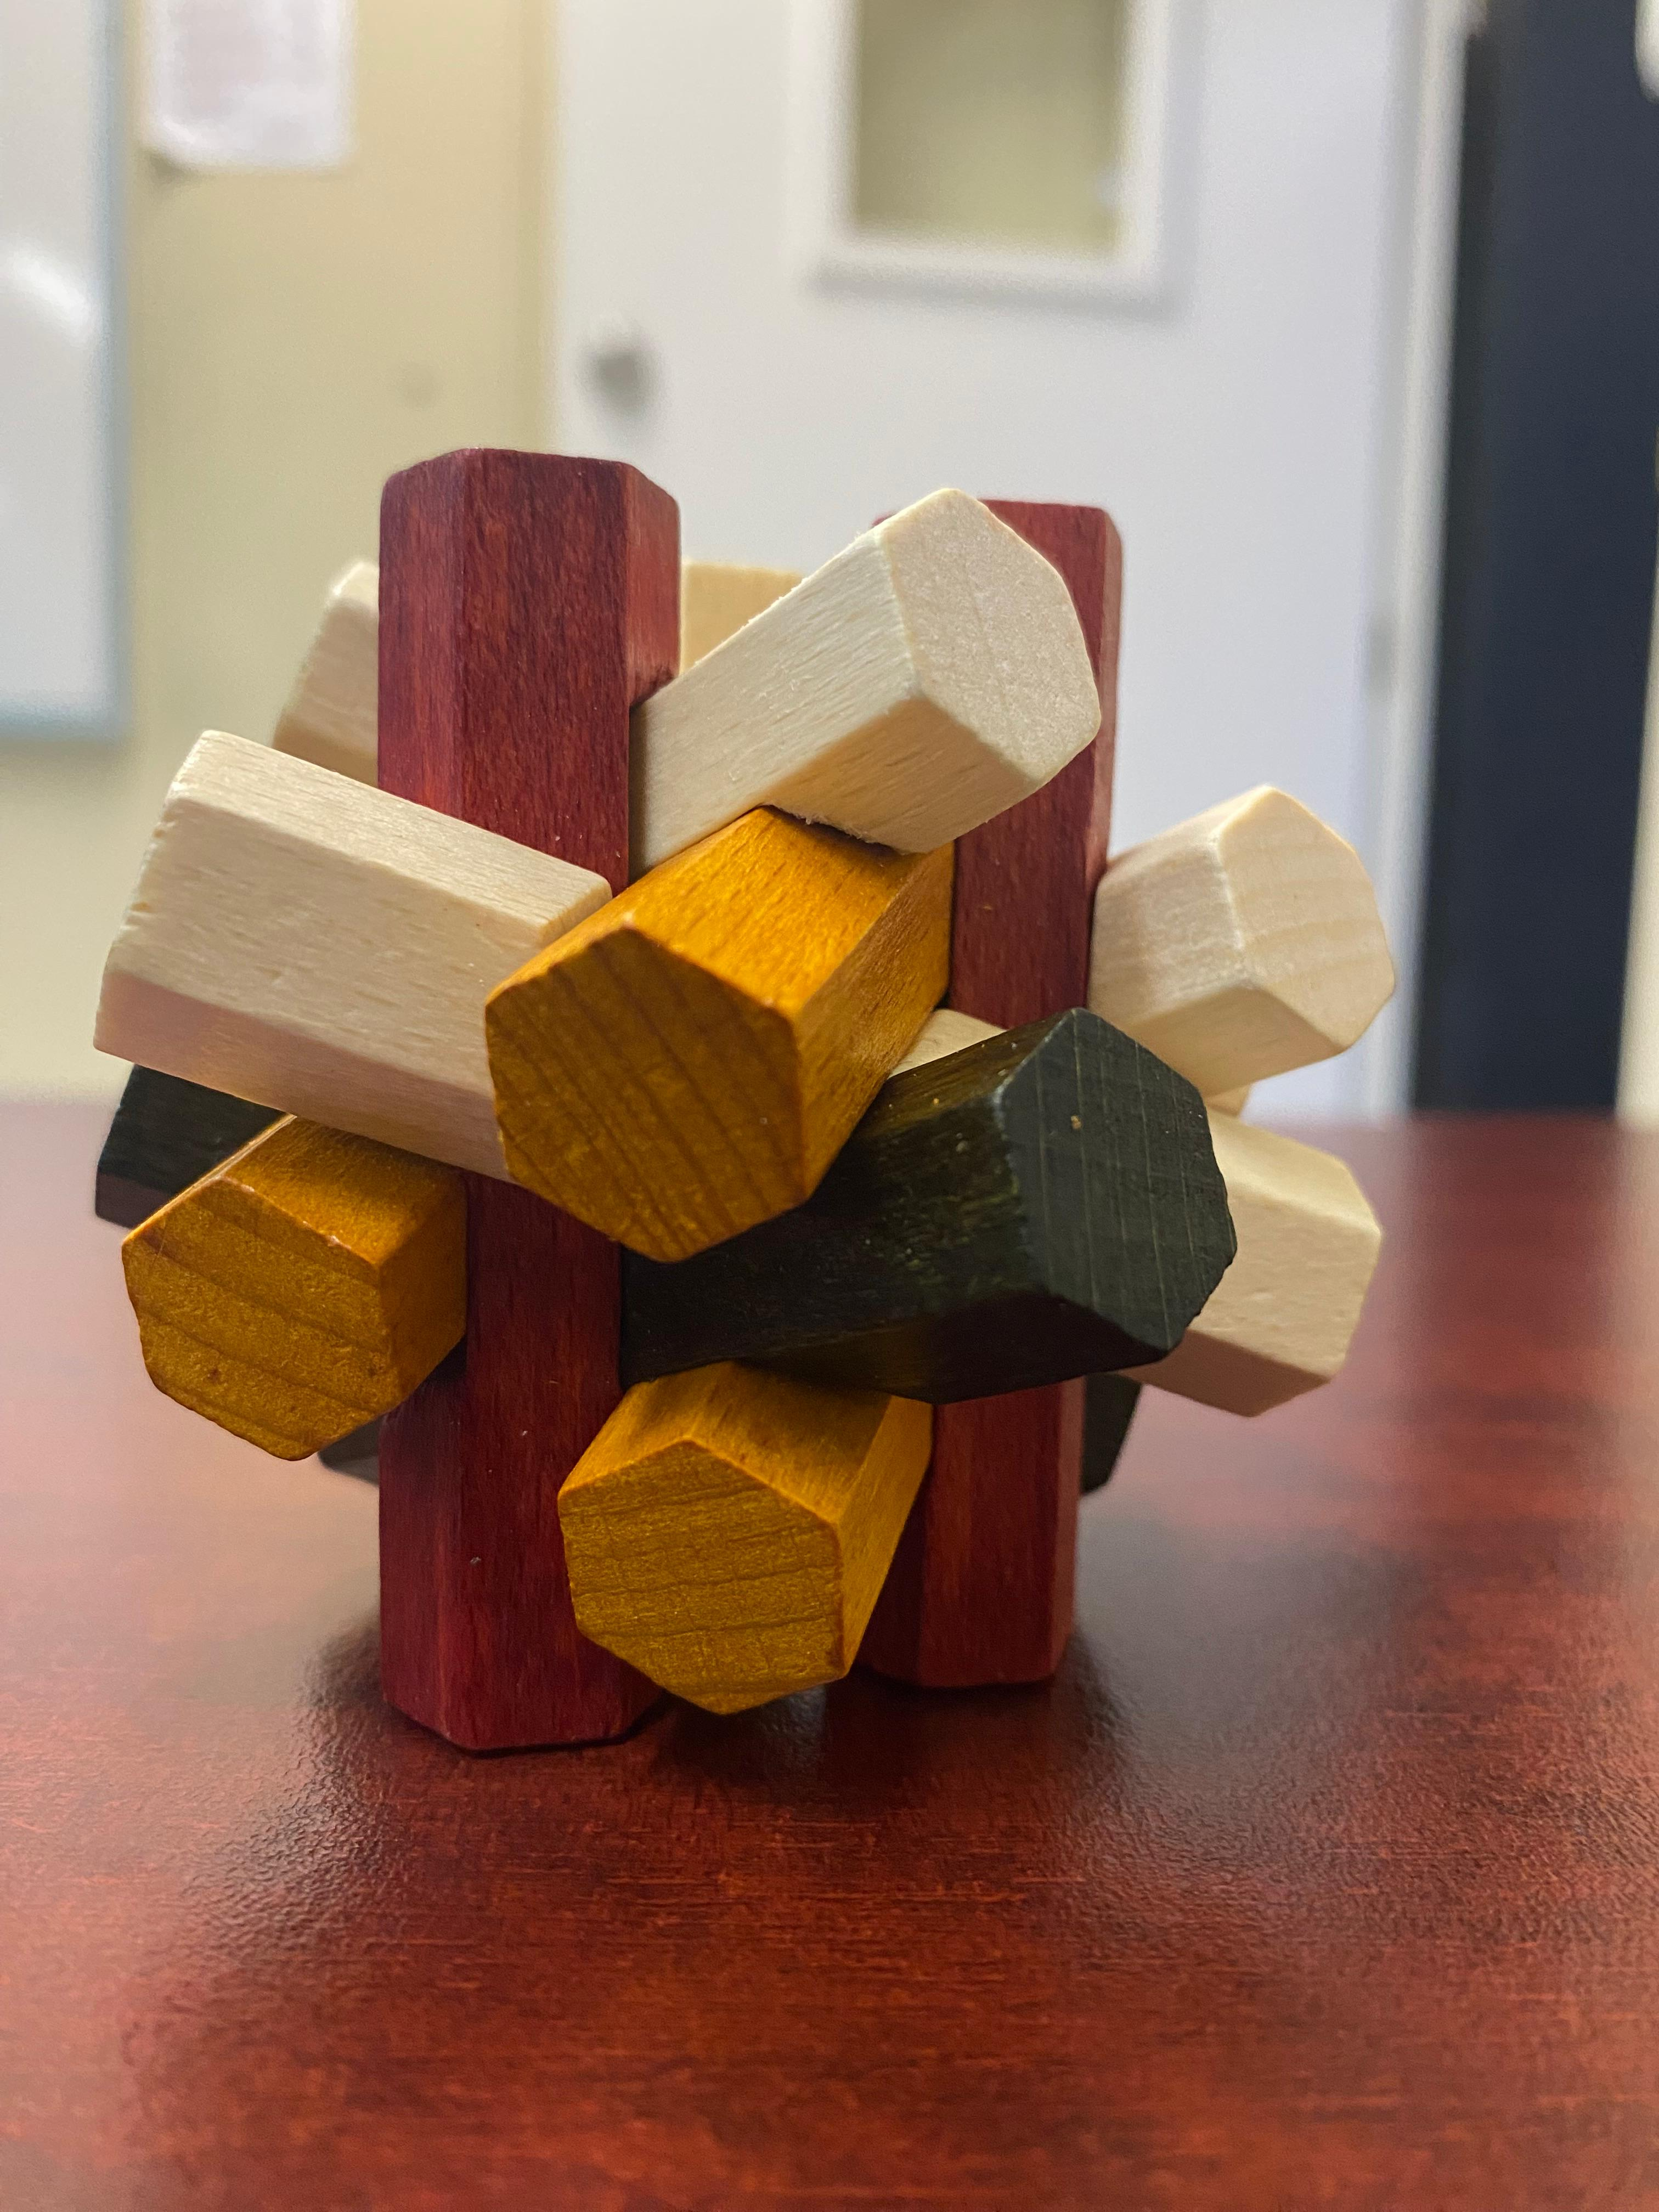
\includegraphics[scale = 0.04]{clase7/R1-1.jpeg}&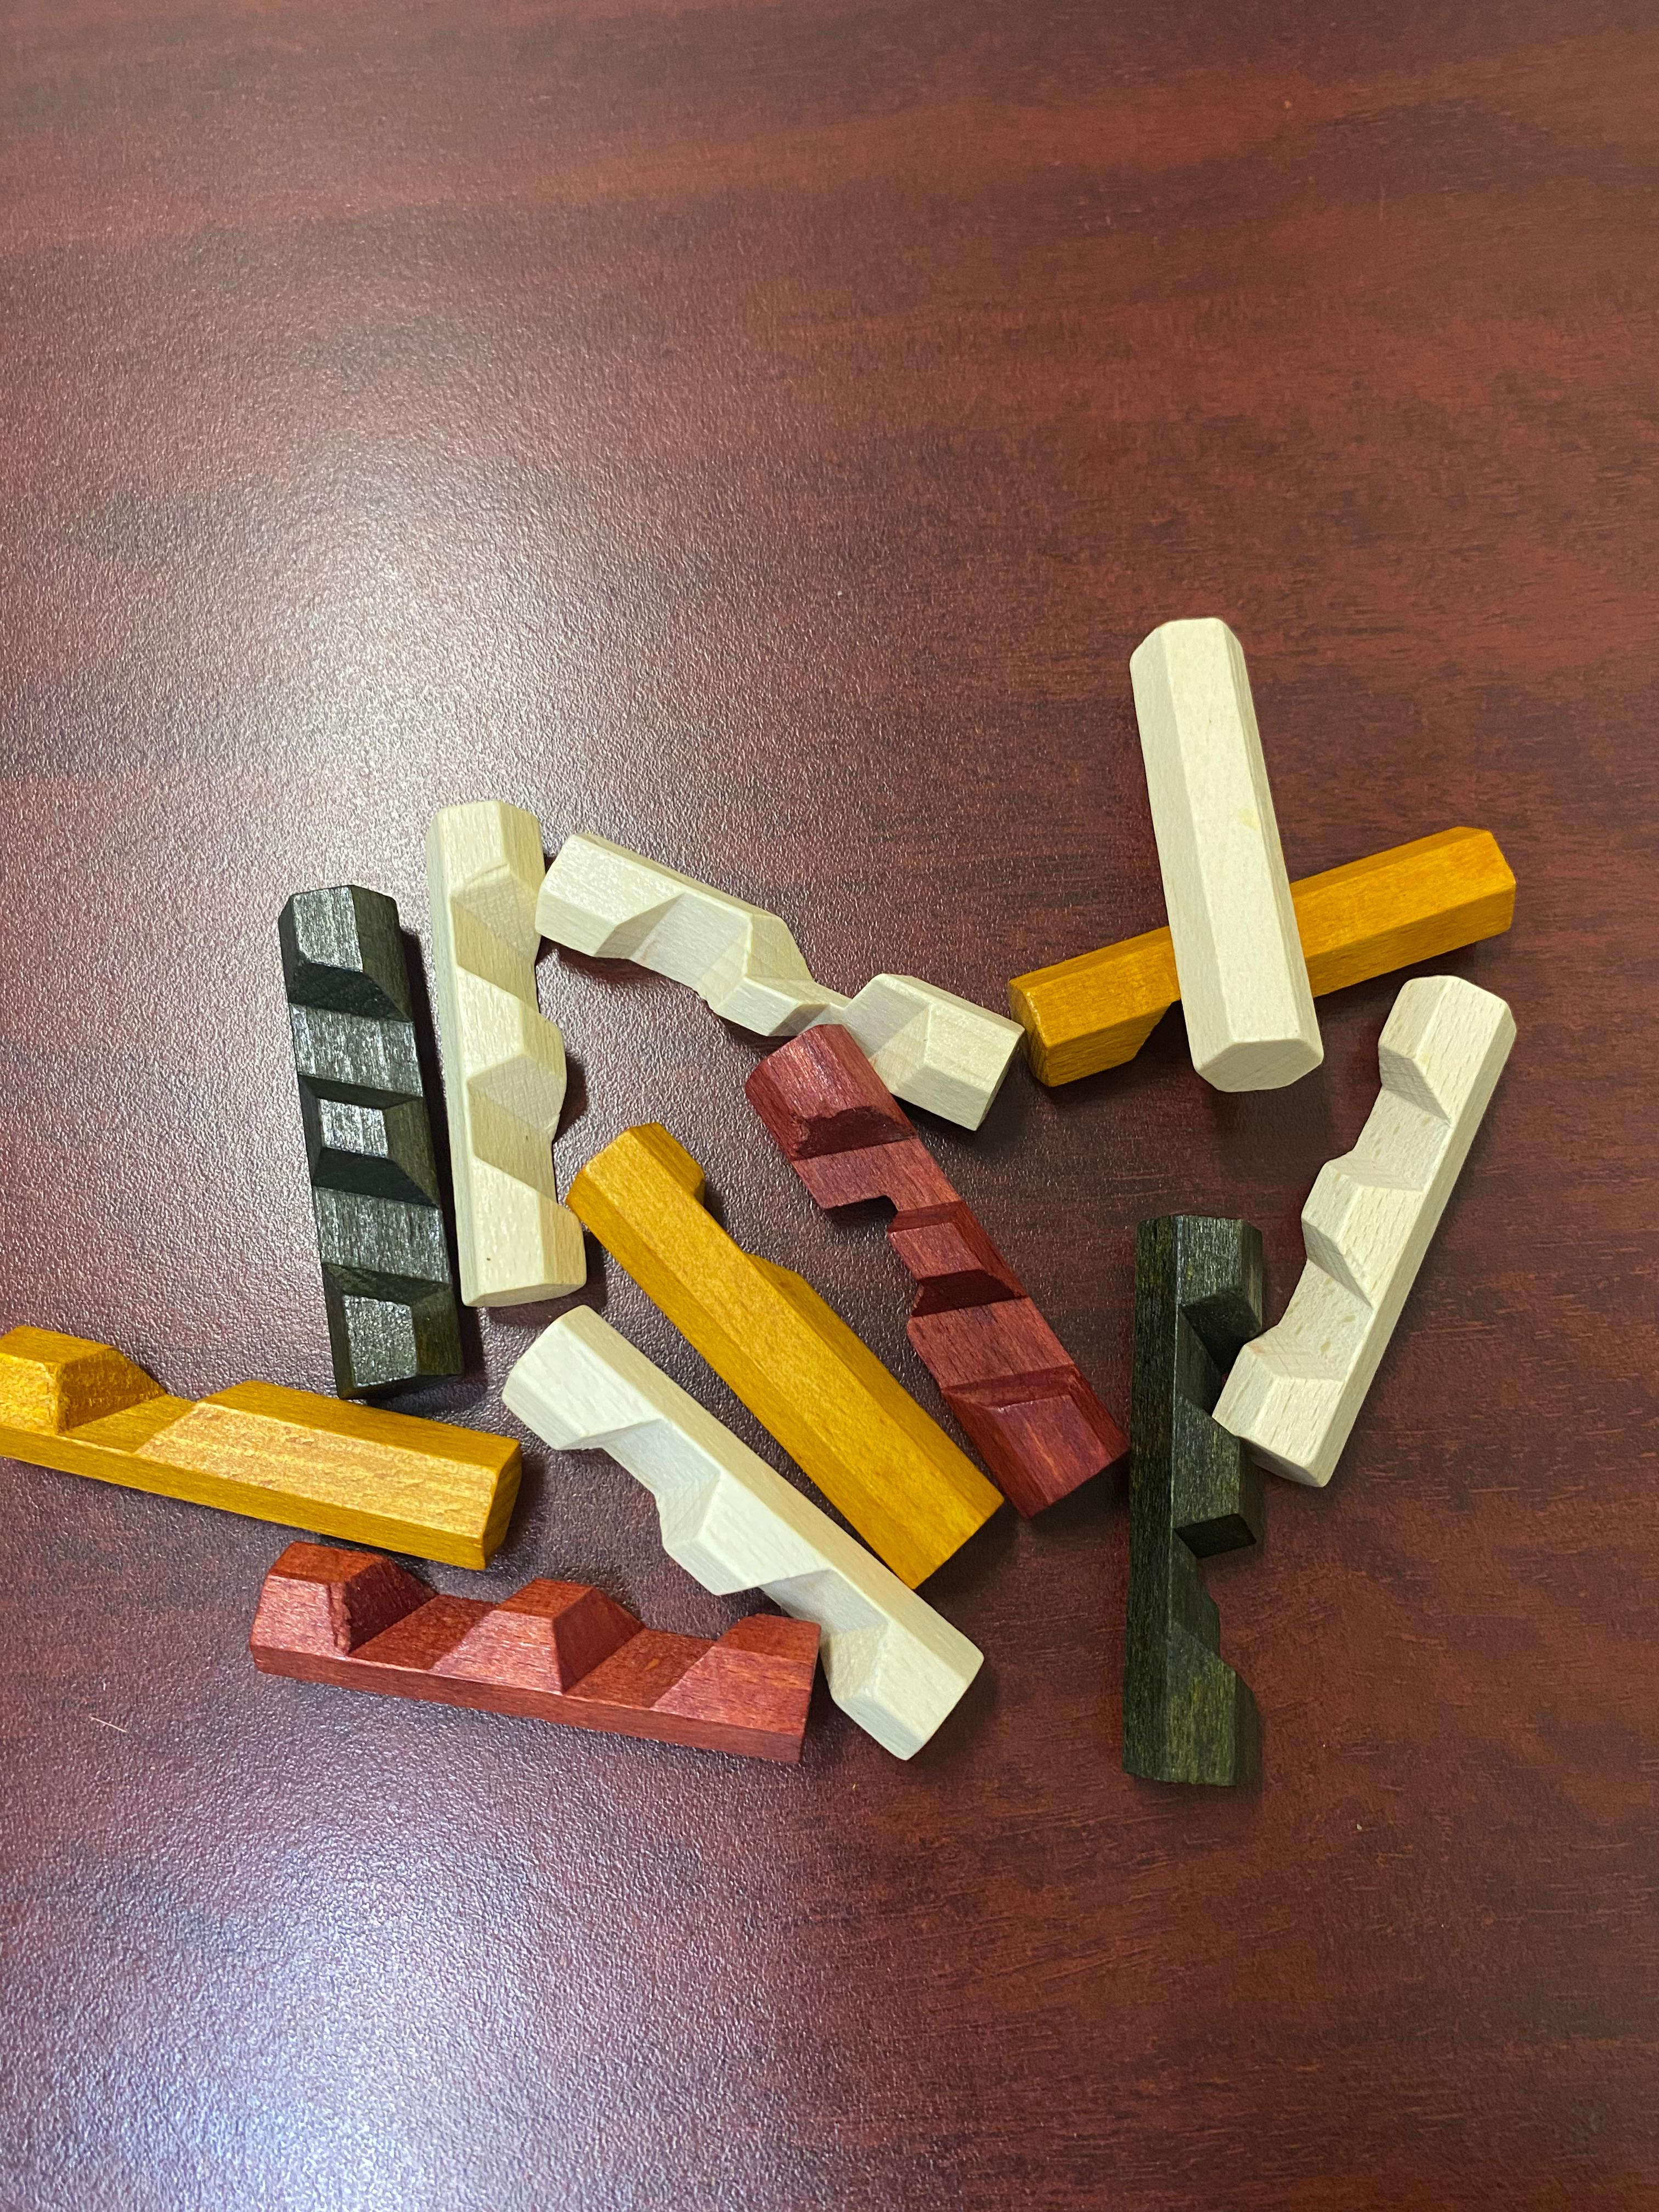
\includegraphics[scale = 0.04]{clase7/R1-2.jpeg}
    \end{tabular}
    \caption{}
\end{figure}

Debido a que en el primer problema me llevé alrededor de una hora y 15 minutos, sólo pude armar tres rompecabezas más

\section{Rompecabezas 2}

Sin desensamblar el cubo lo fui observando, moviendo cada pieza ligeramente para intentar ver cómo se conectaban. Luego lo deshice para comenzar con el proceso de armado y por mis observaciones, las piezas que iban en las esquinas del cubo tenían forma de L y a partir de ahí solo fui haciendo permutaciones respecto a la posición de cada pieza.

\begin{figure}[H]
    \begin{tabular}{ccc}
        Inico & Proceso & Final\\\\
        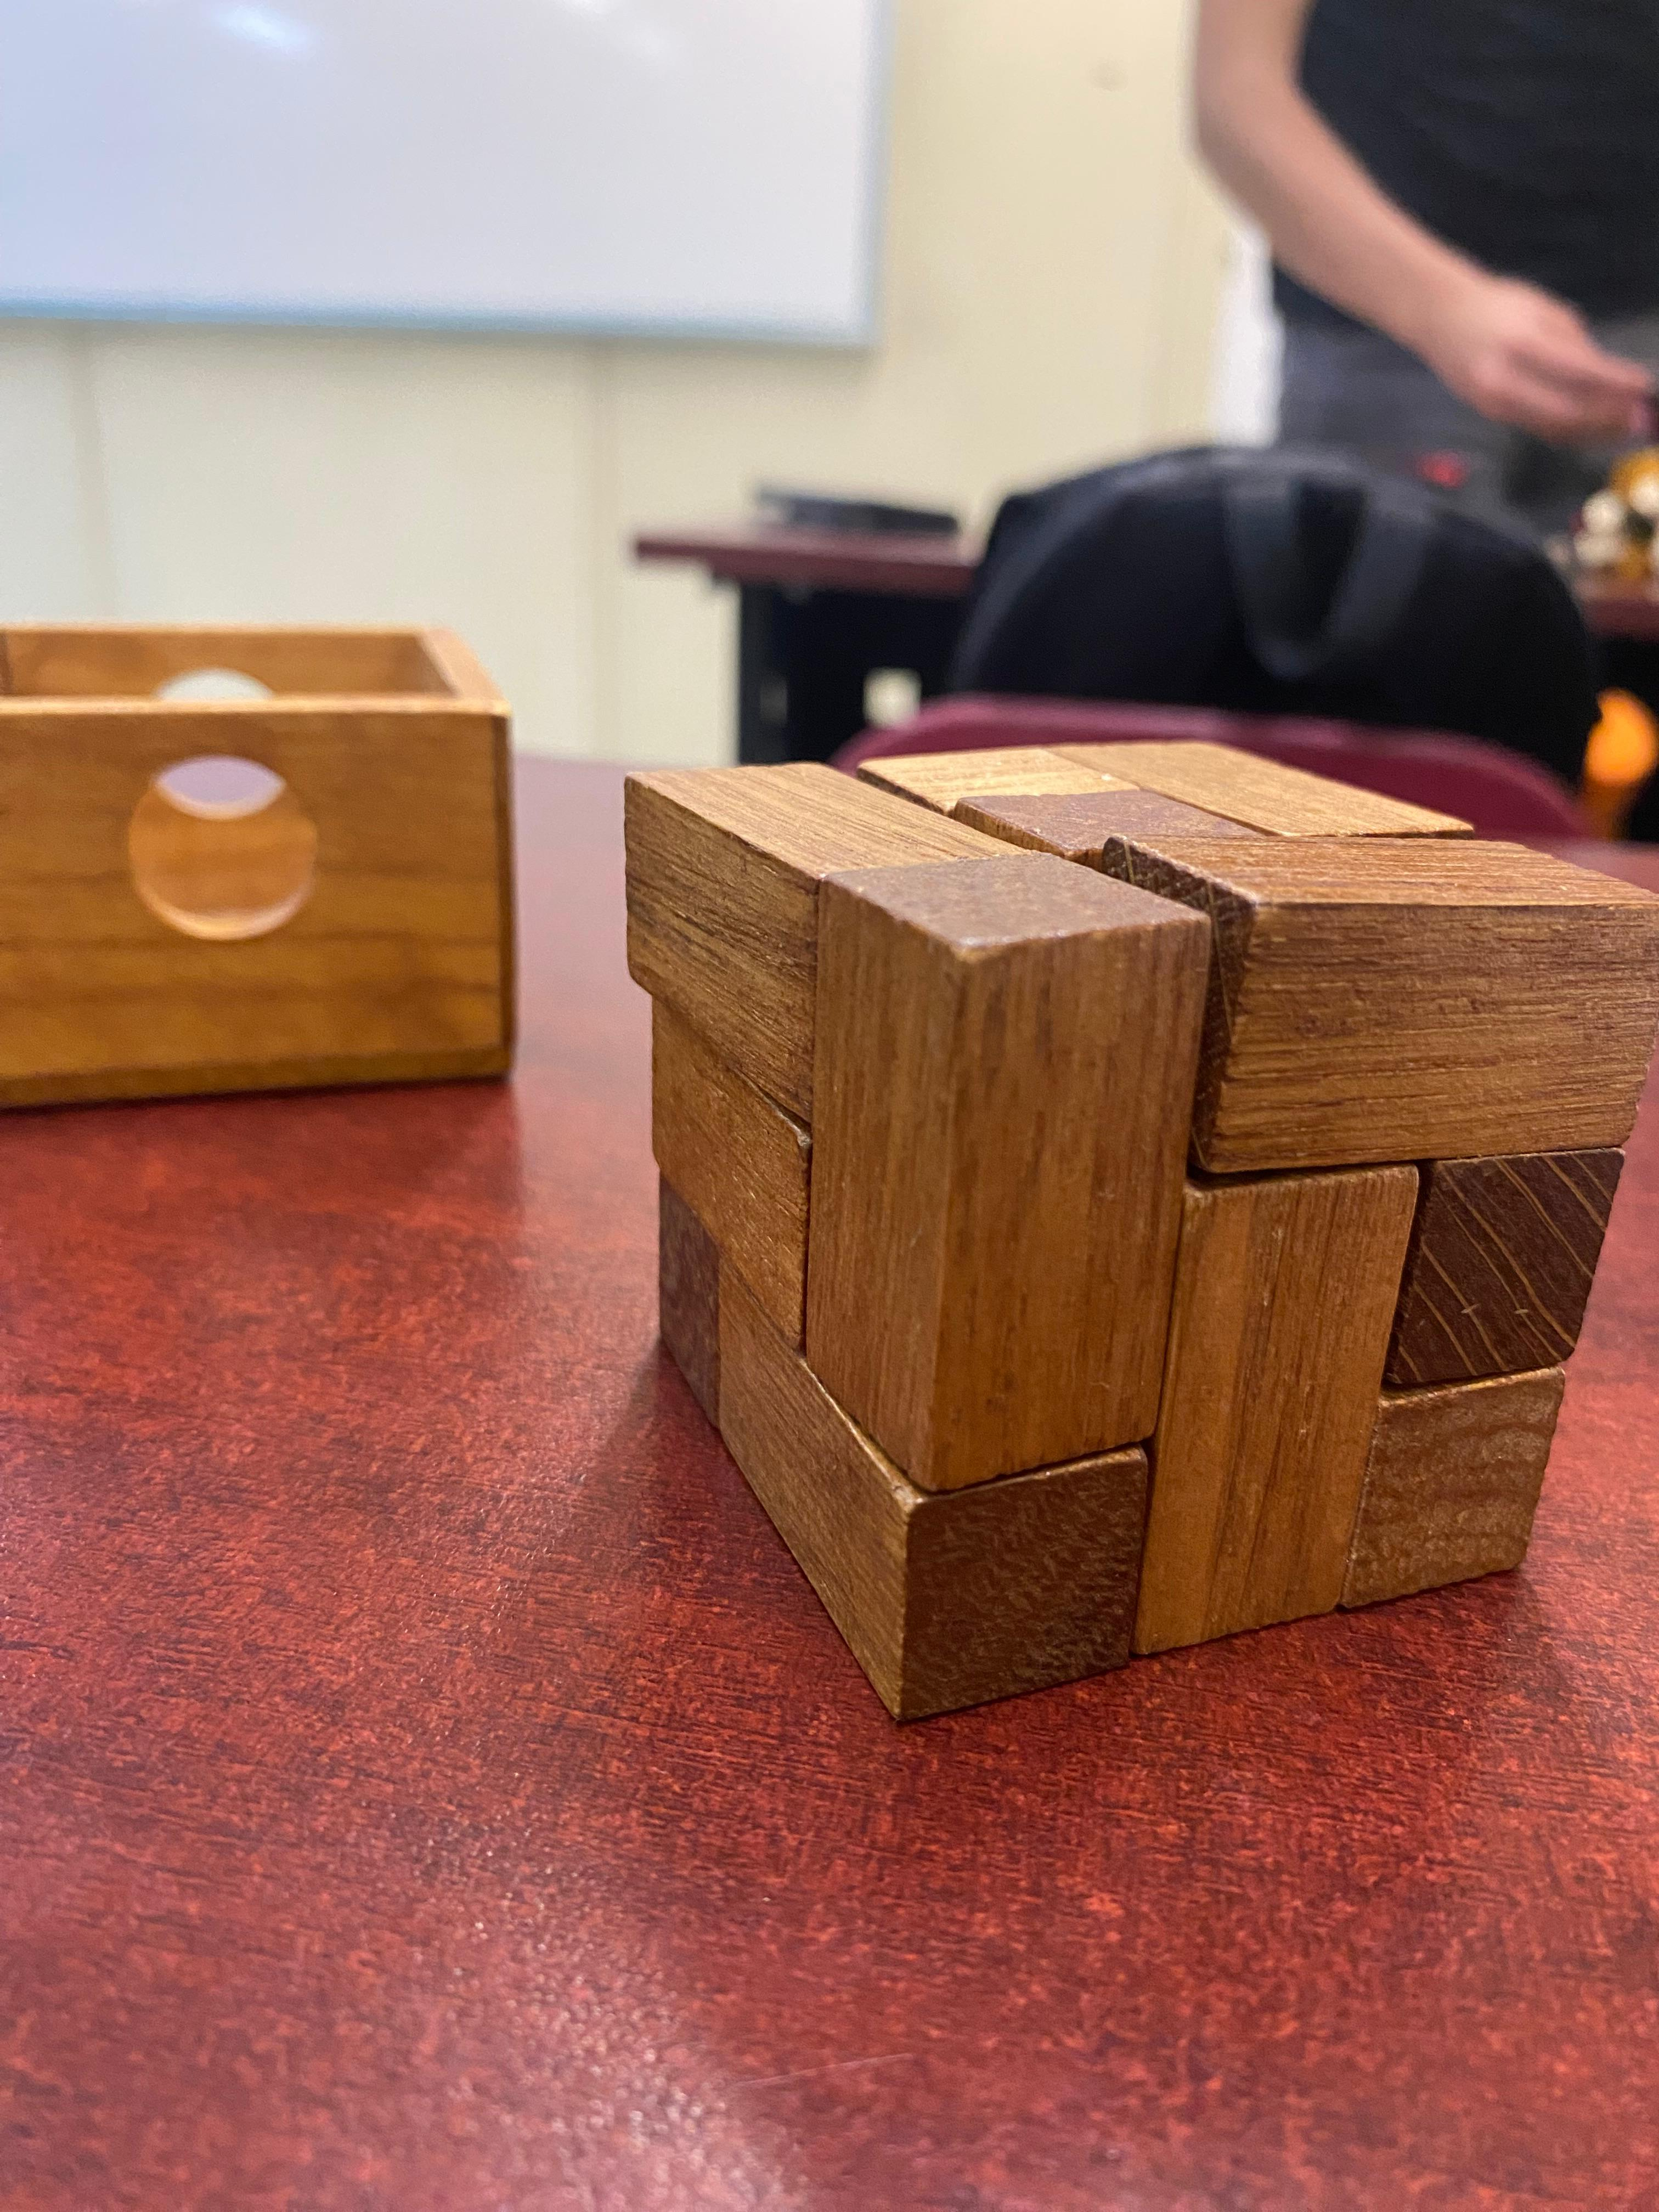
\includegraphics[scale = 0.04]{clase7/R2Inicio.jpeg}&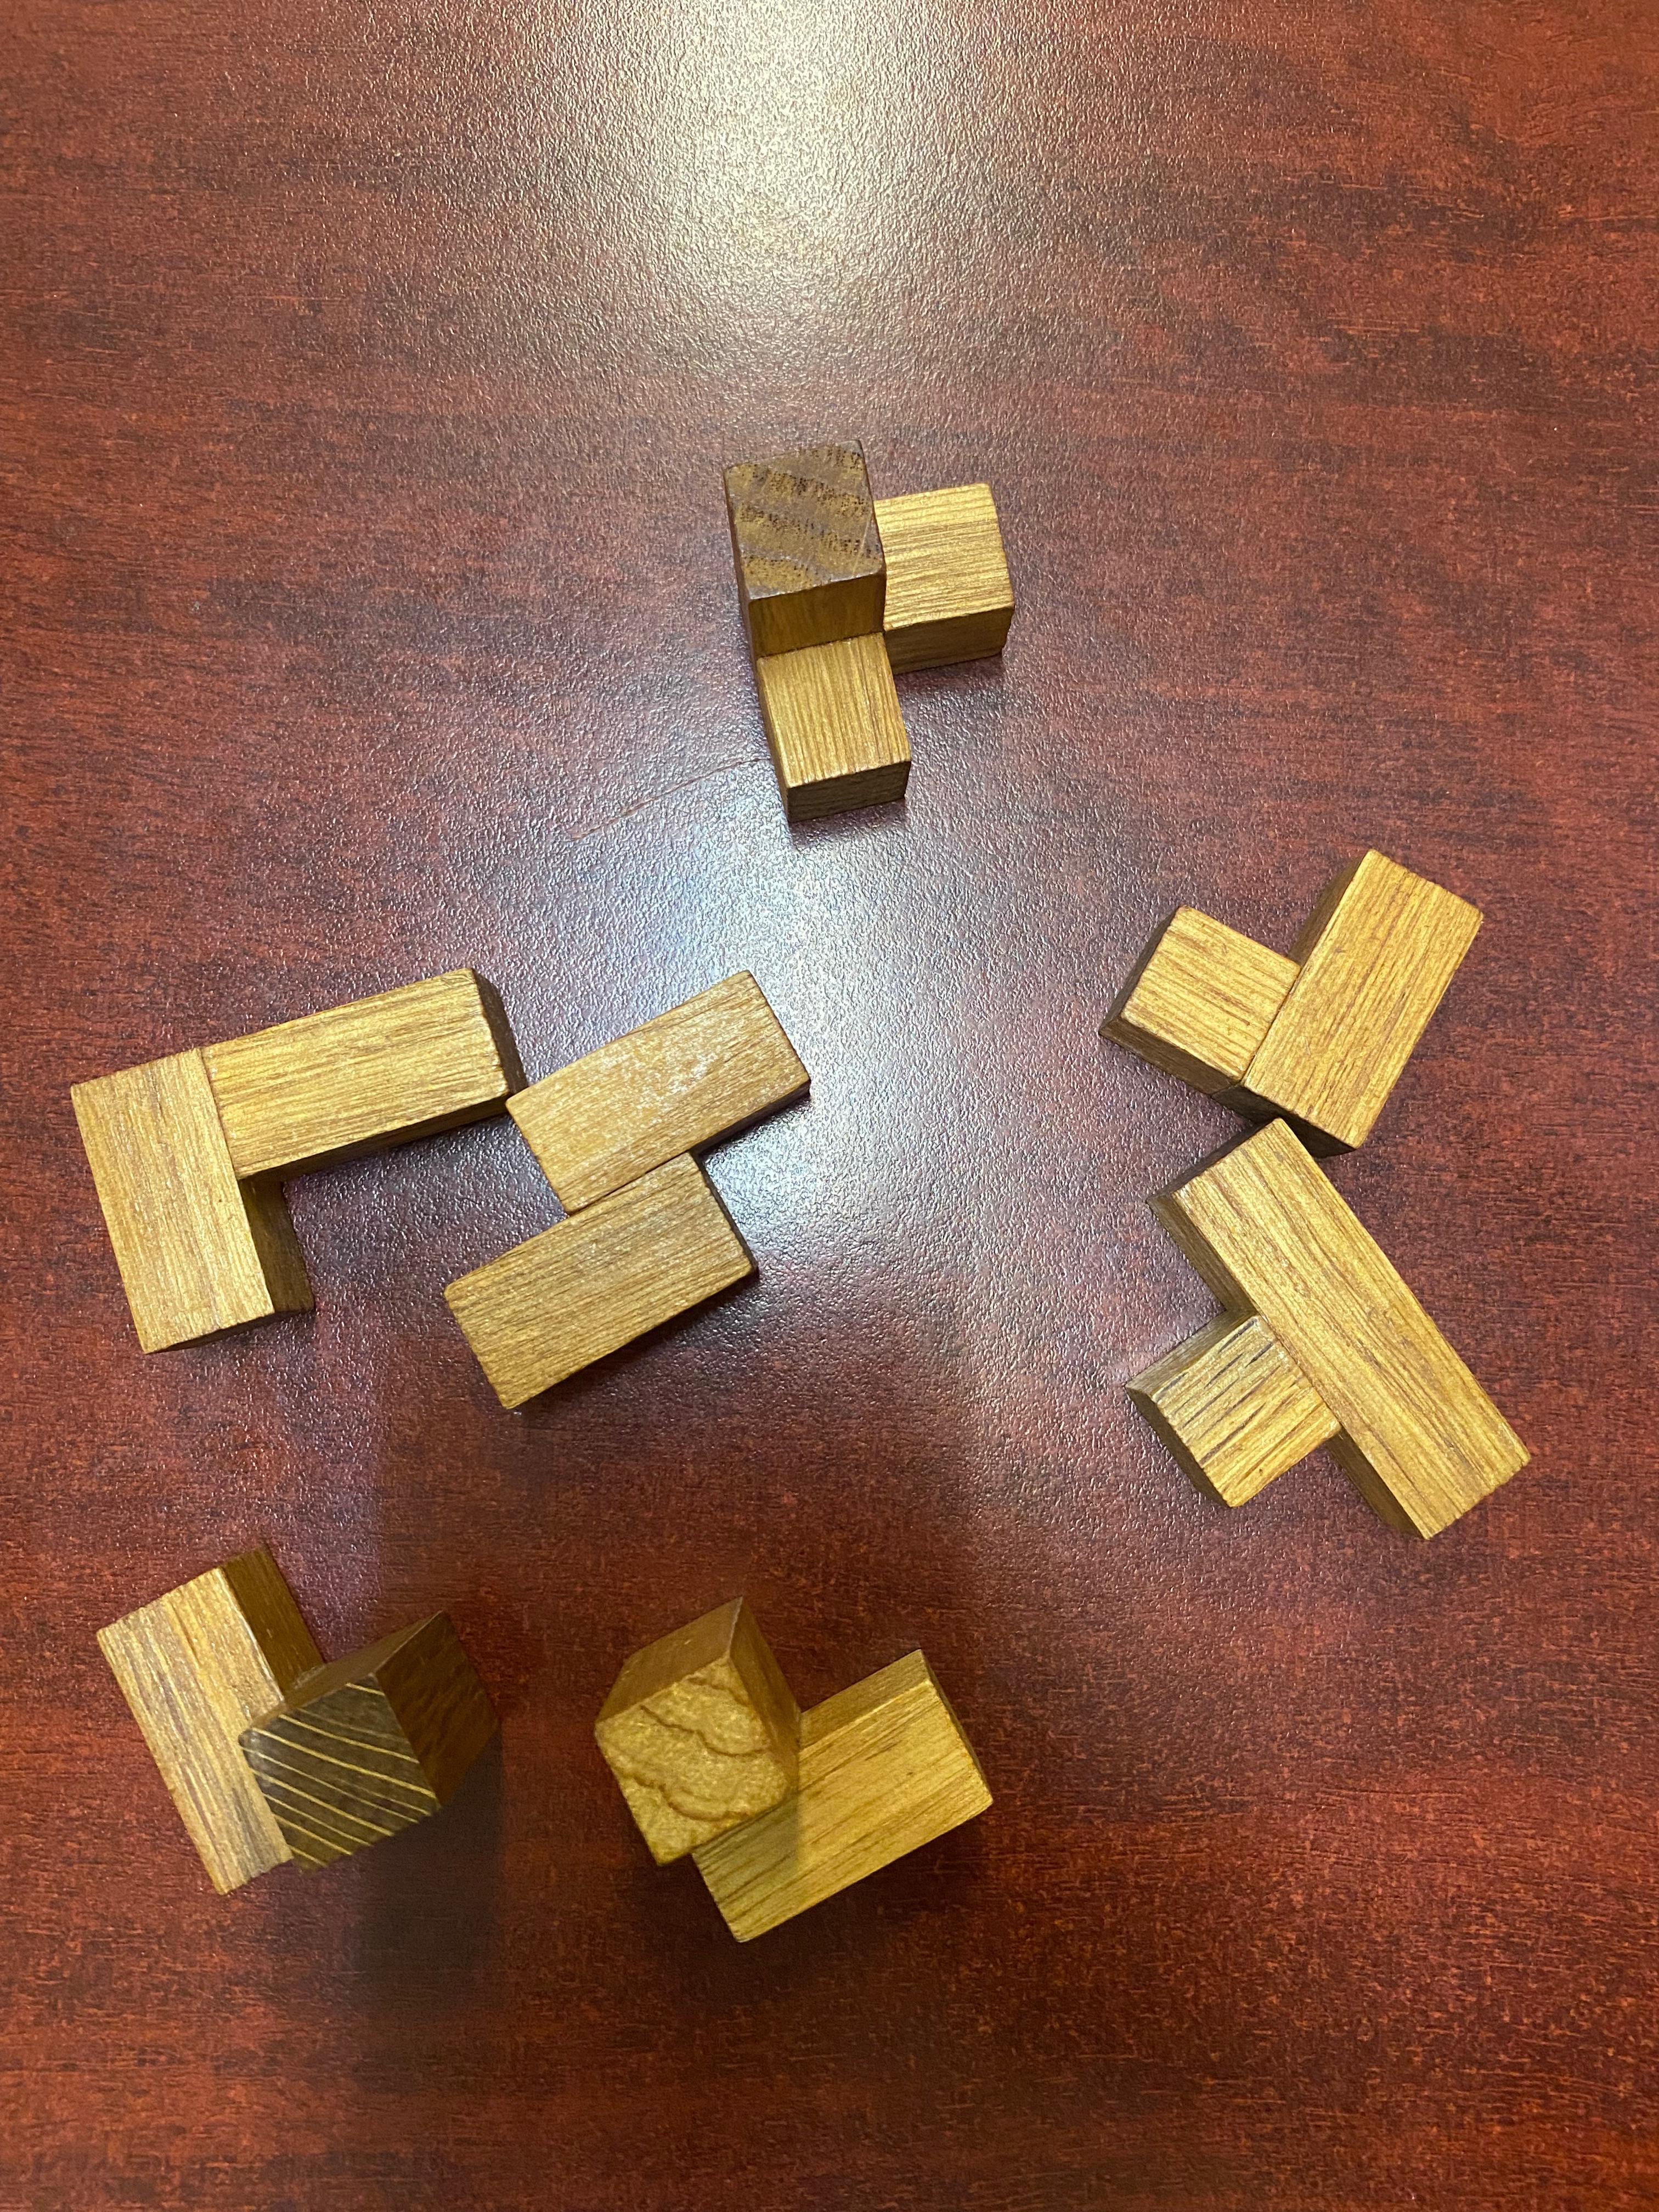
\includegraphics[scale = 0.04]{clase7/R2Proceso.jpeg}&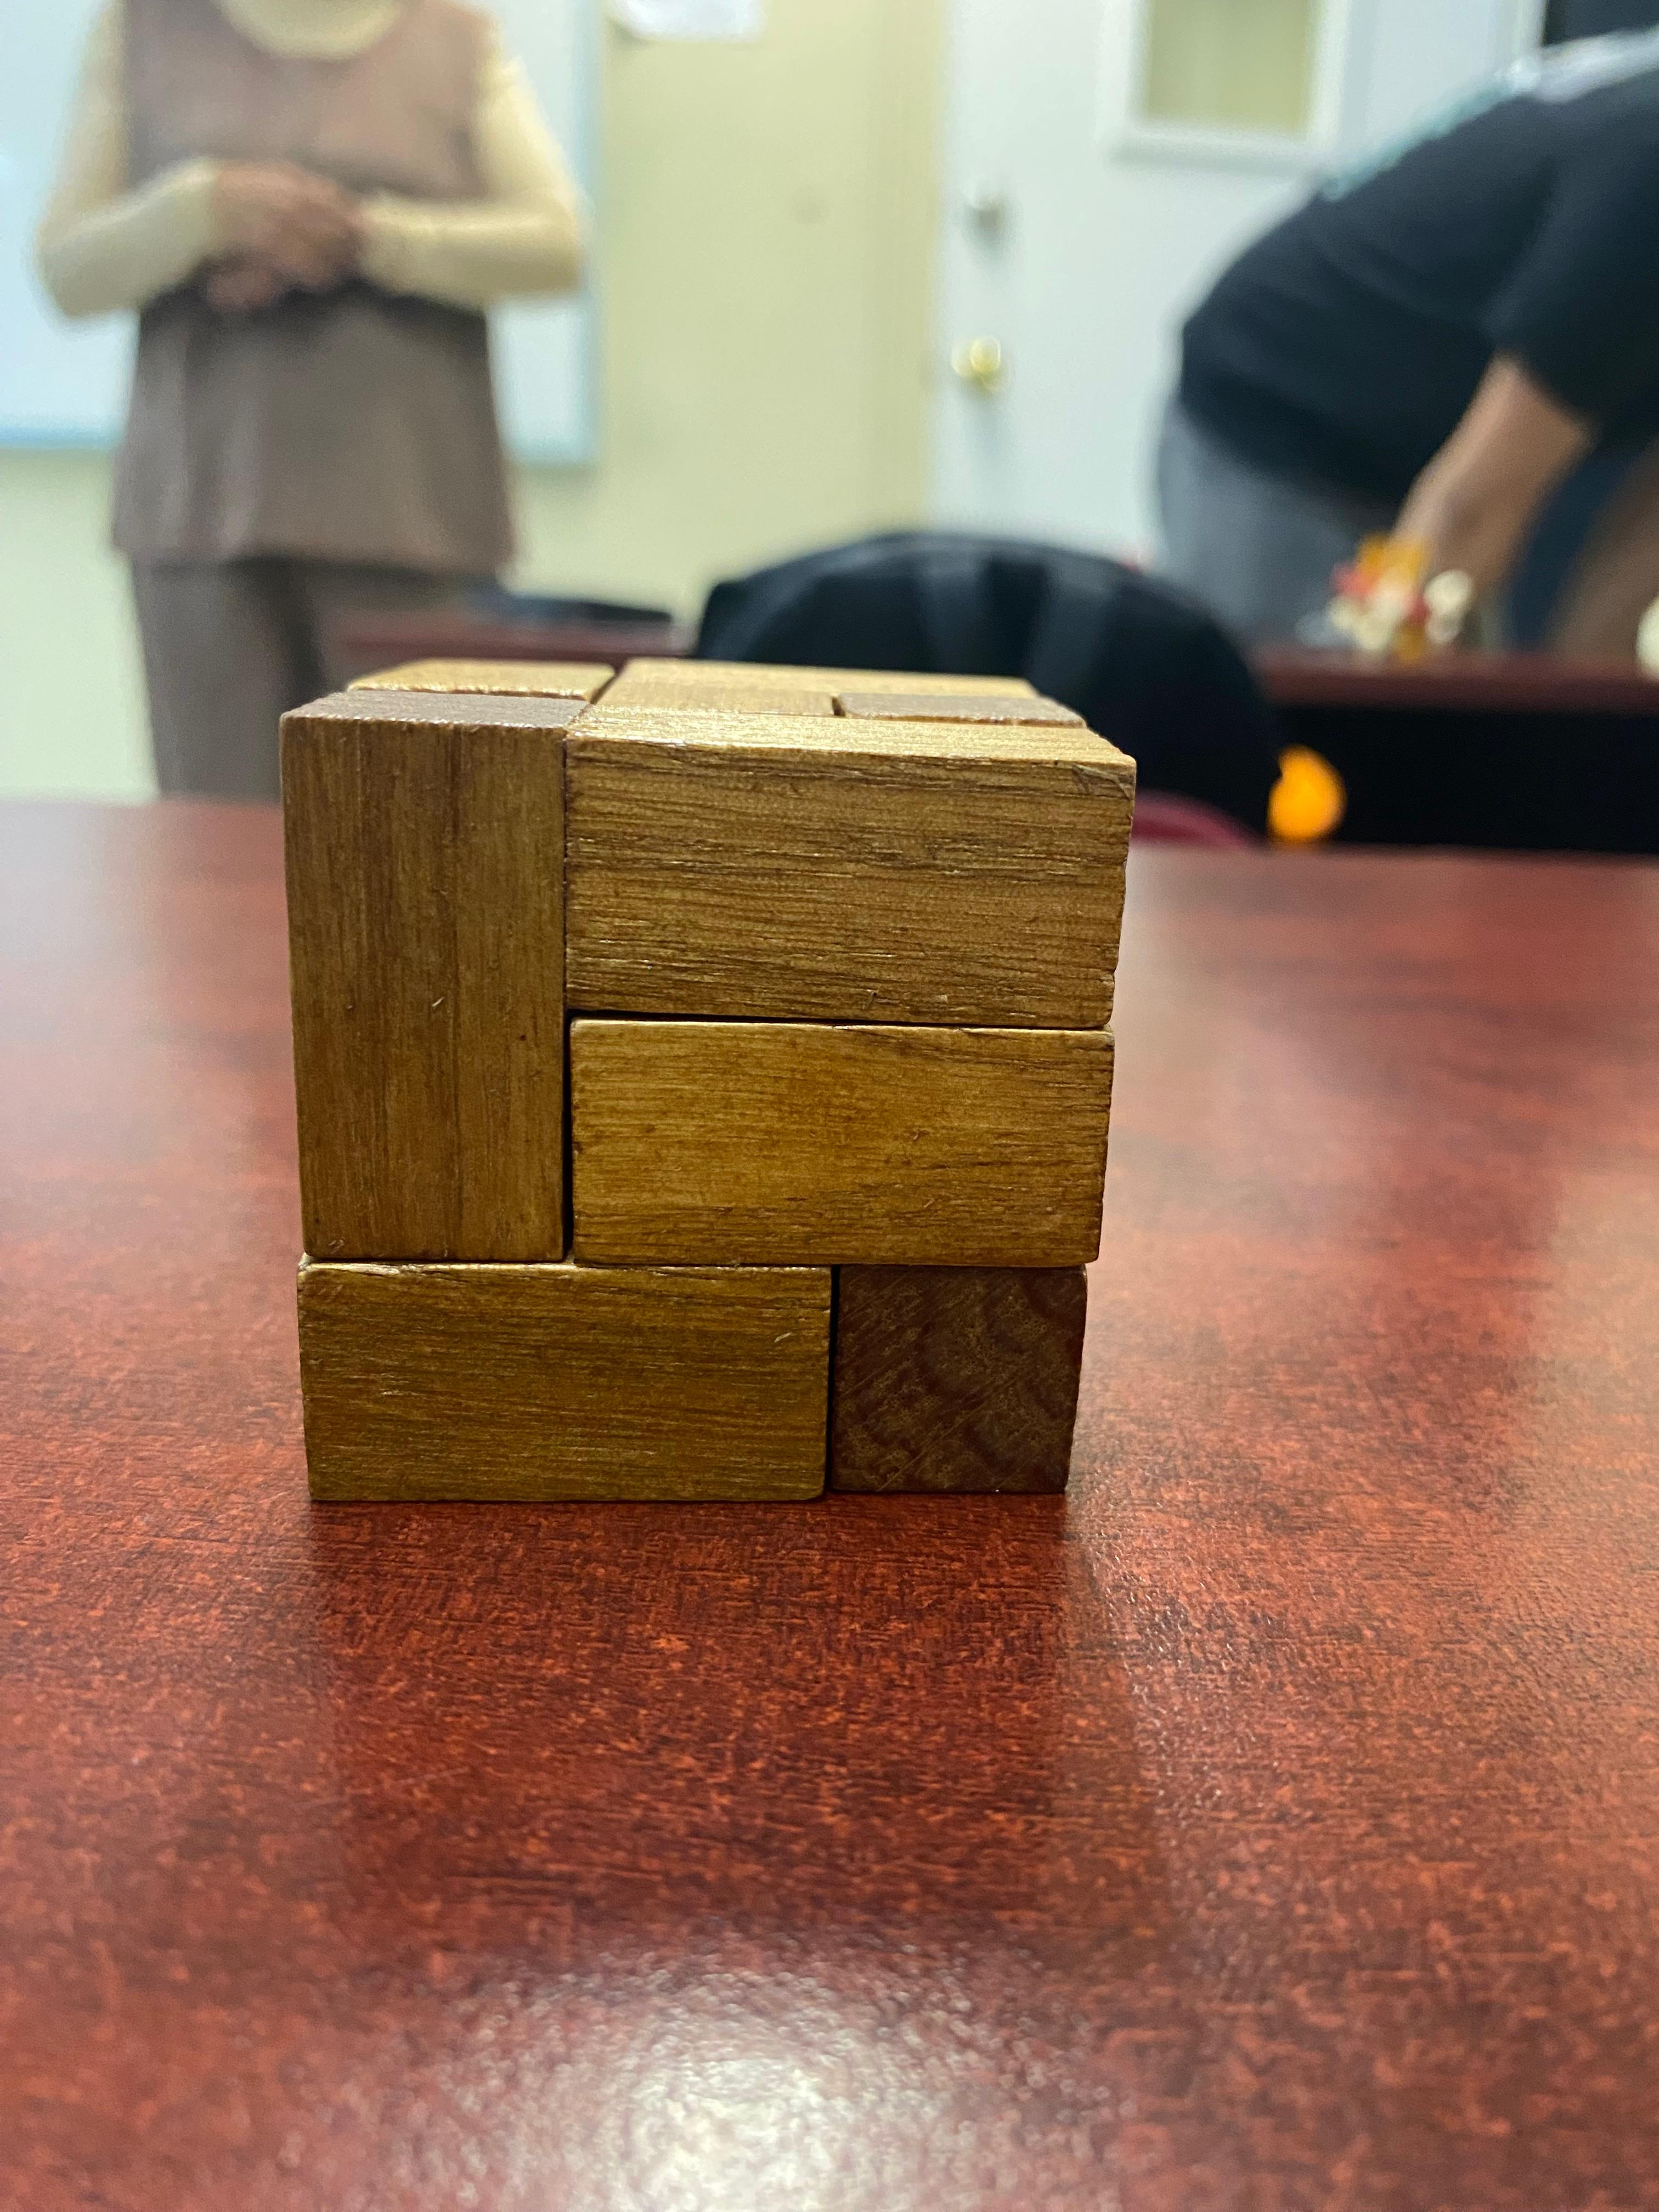
\includegraphics[scale = 0.04]{clase7/R2Final.jpeg}
    \end{tabular}
    \caption{}
\end{figure}

\section{Rompecabezas 3}

Este rompecabezas iniciaba con cuatro T las cuales debía acomodar dentro del tablero sin que se salieran ni se amontonaran; Las primeras dos soluciones no me costaron tanto como la tercera.

\begin{figure}[H]
    \begin{tabular}{ccc}
        \multicolumn{3}{c}{SOLUCIONES}\\
        1 & 2 & 3\\\\
        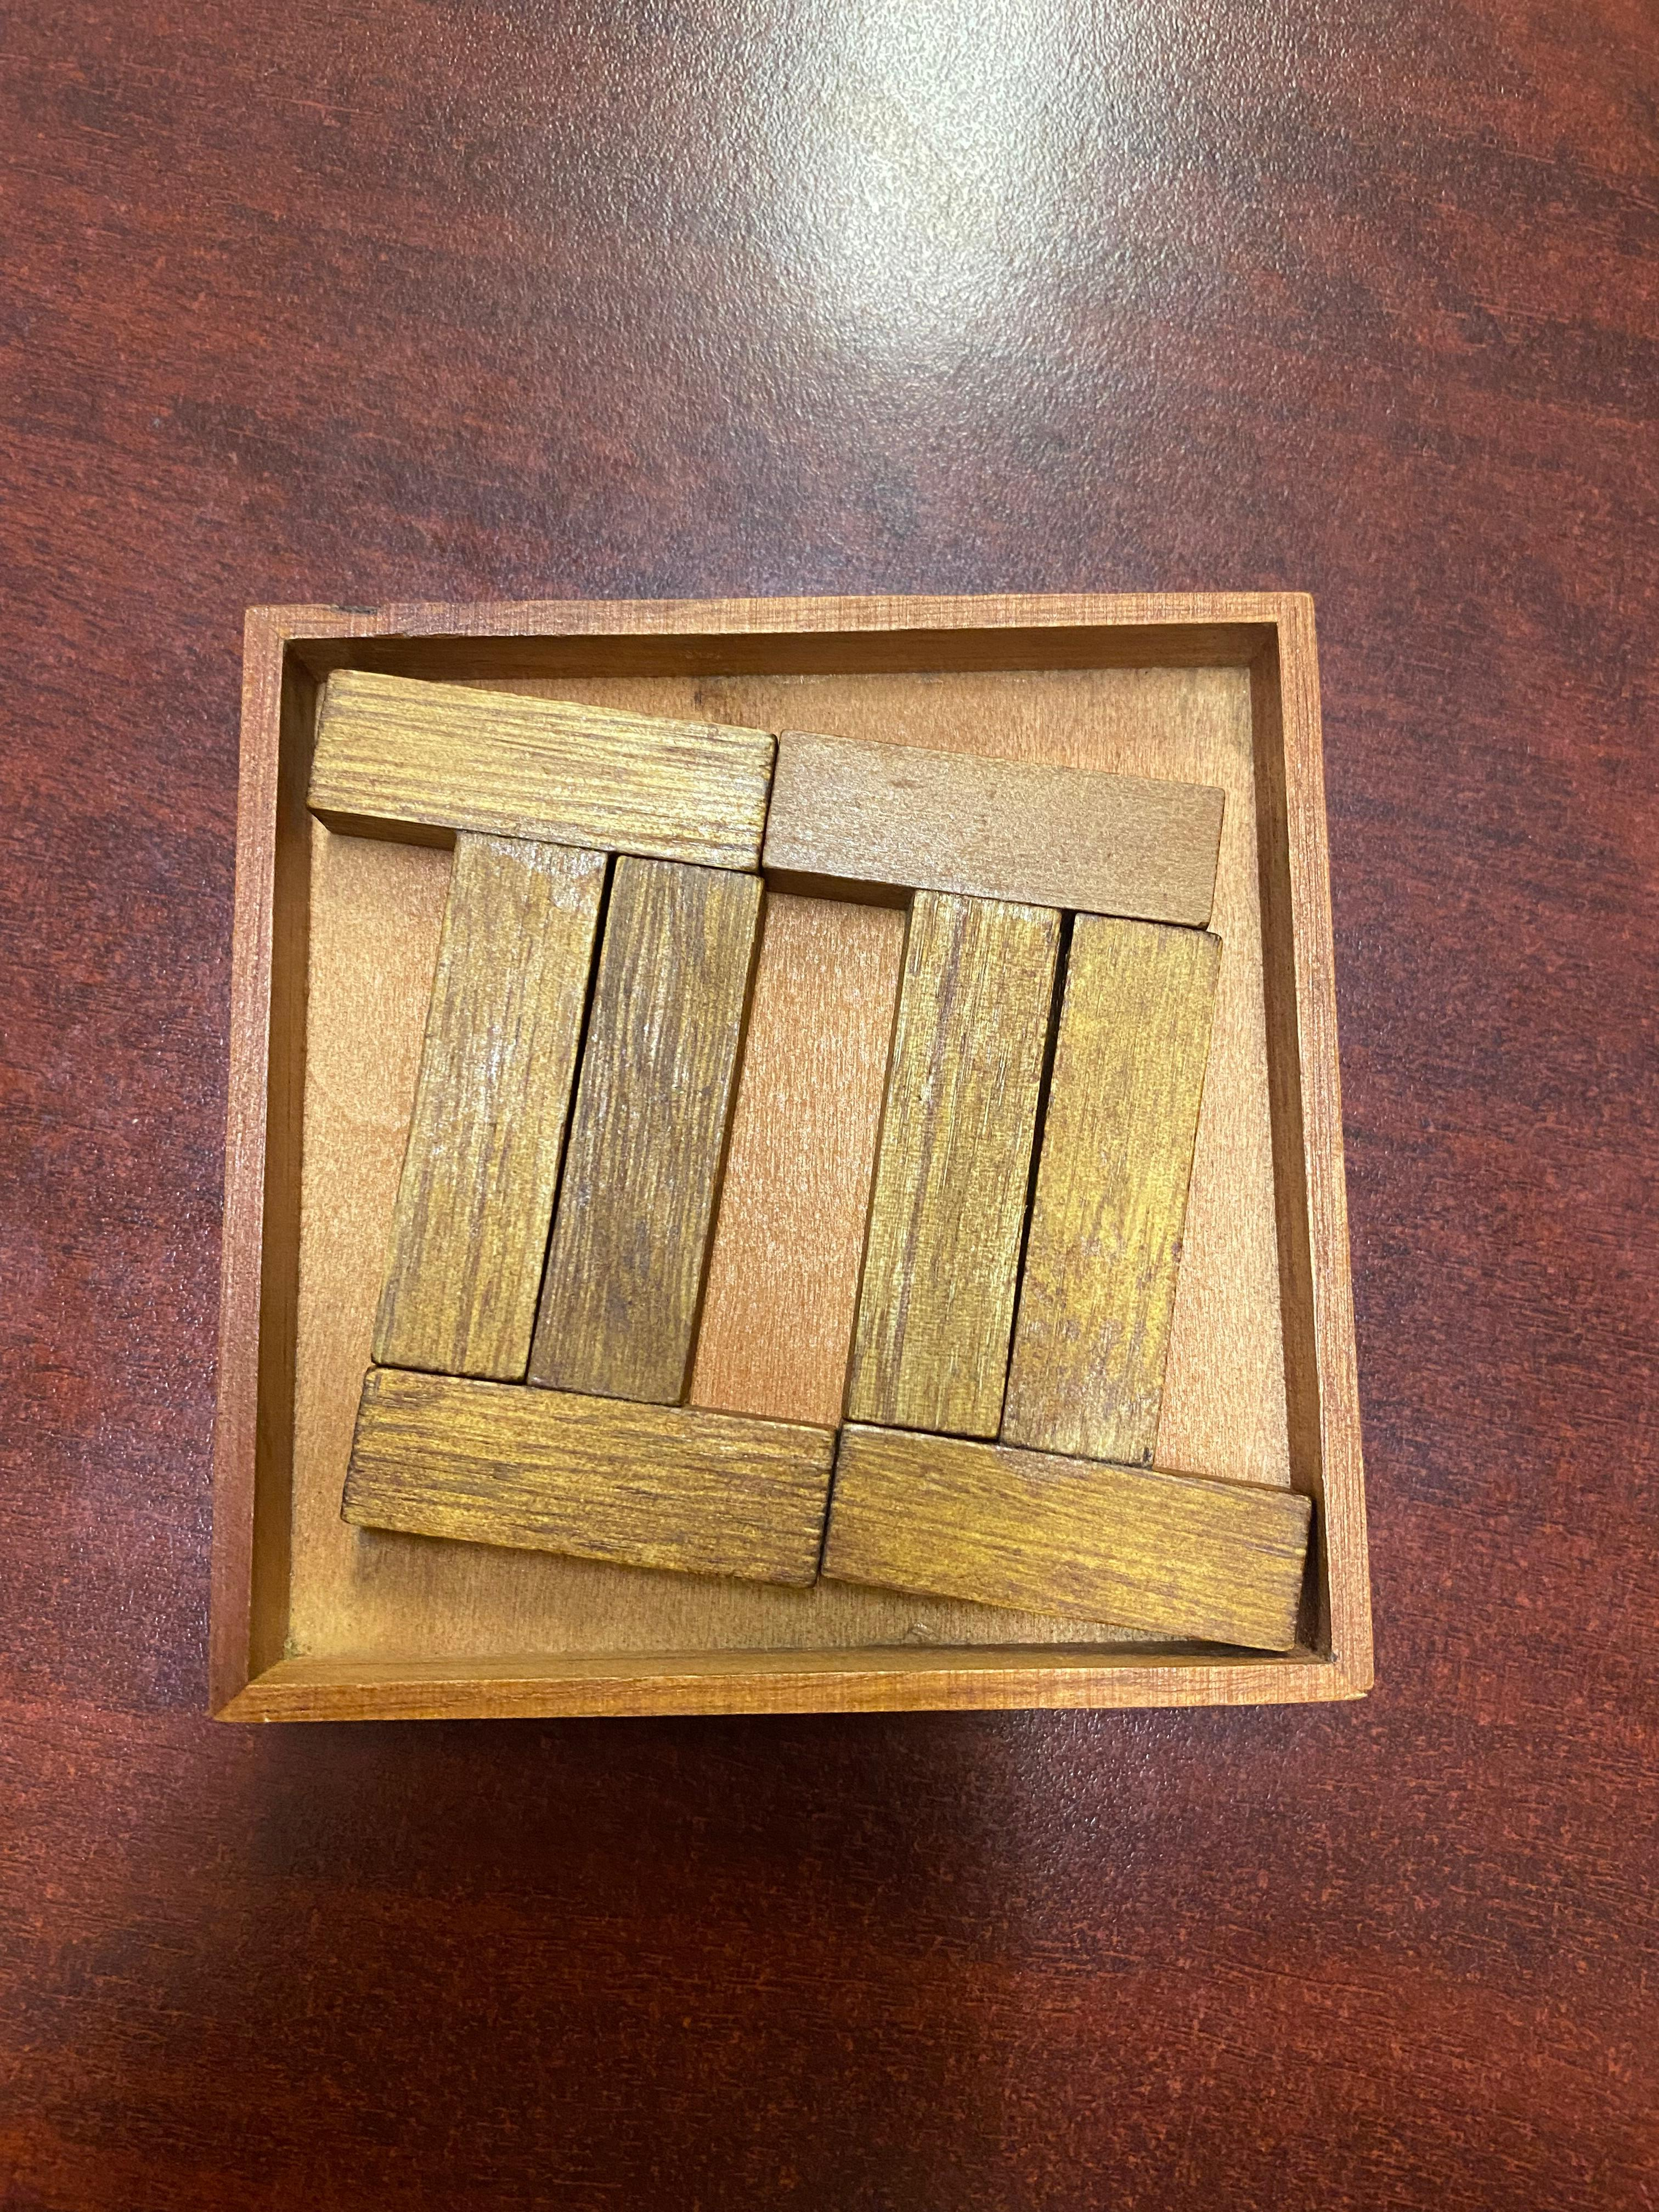
\includegraphics[scale = 0.04]{clase7/R3-Sol1.jpeg}&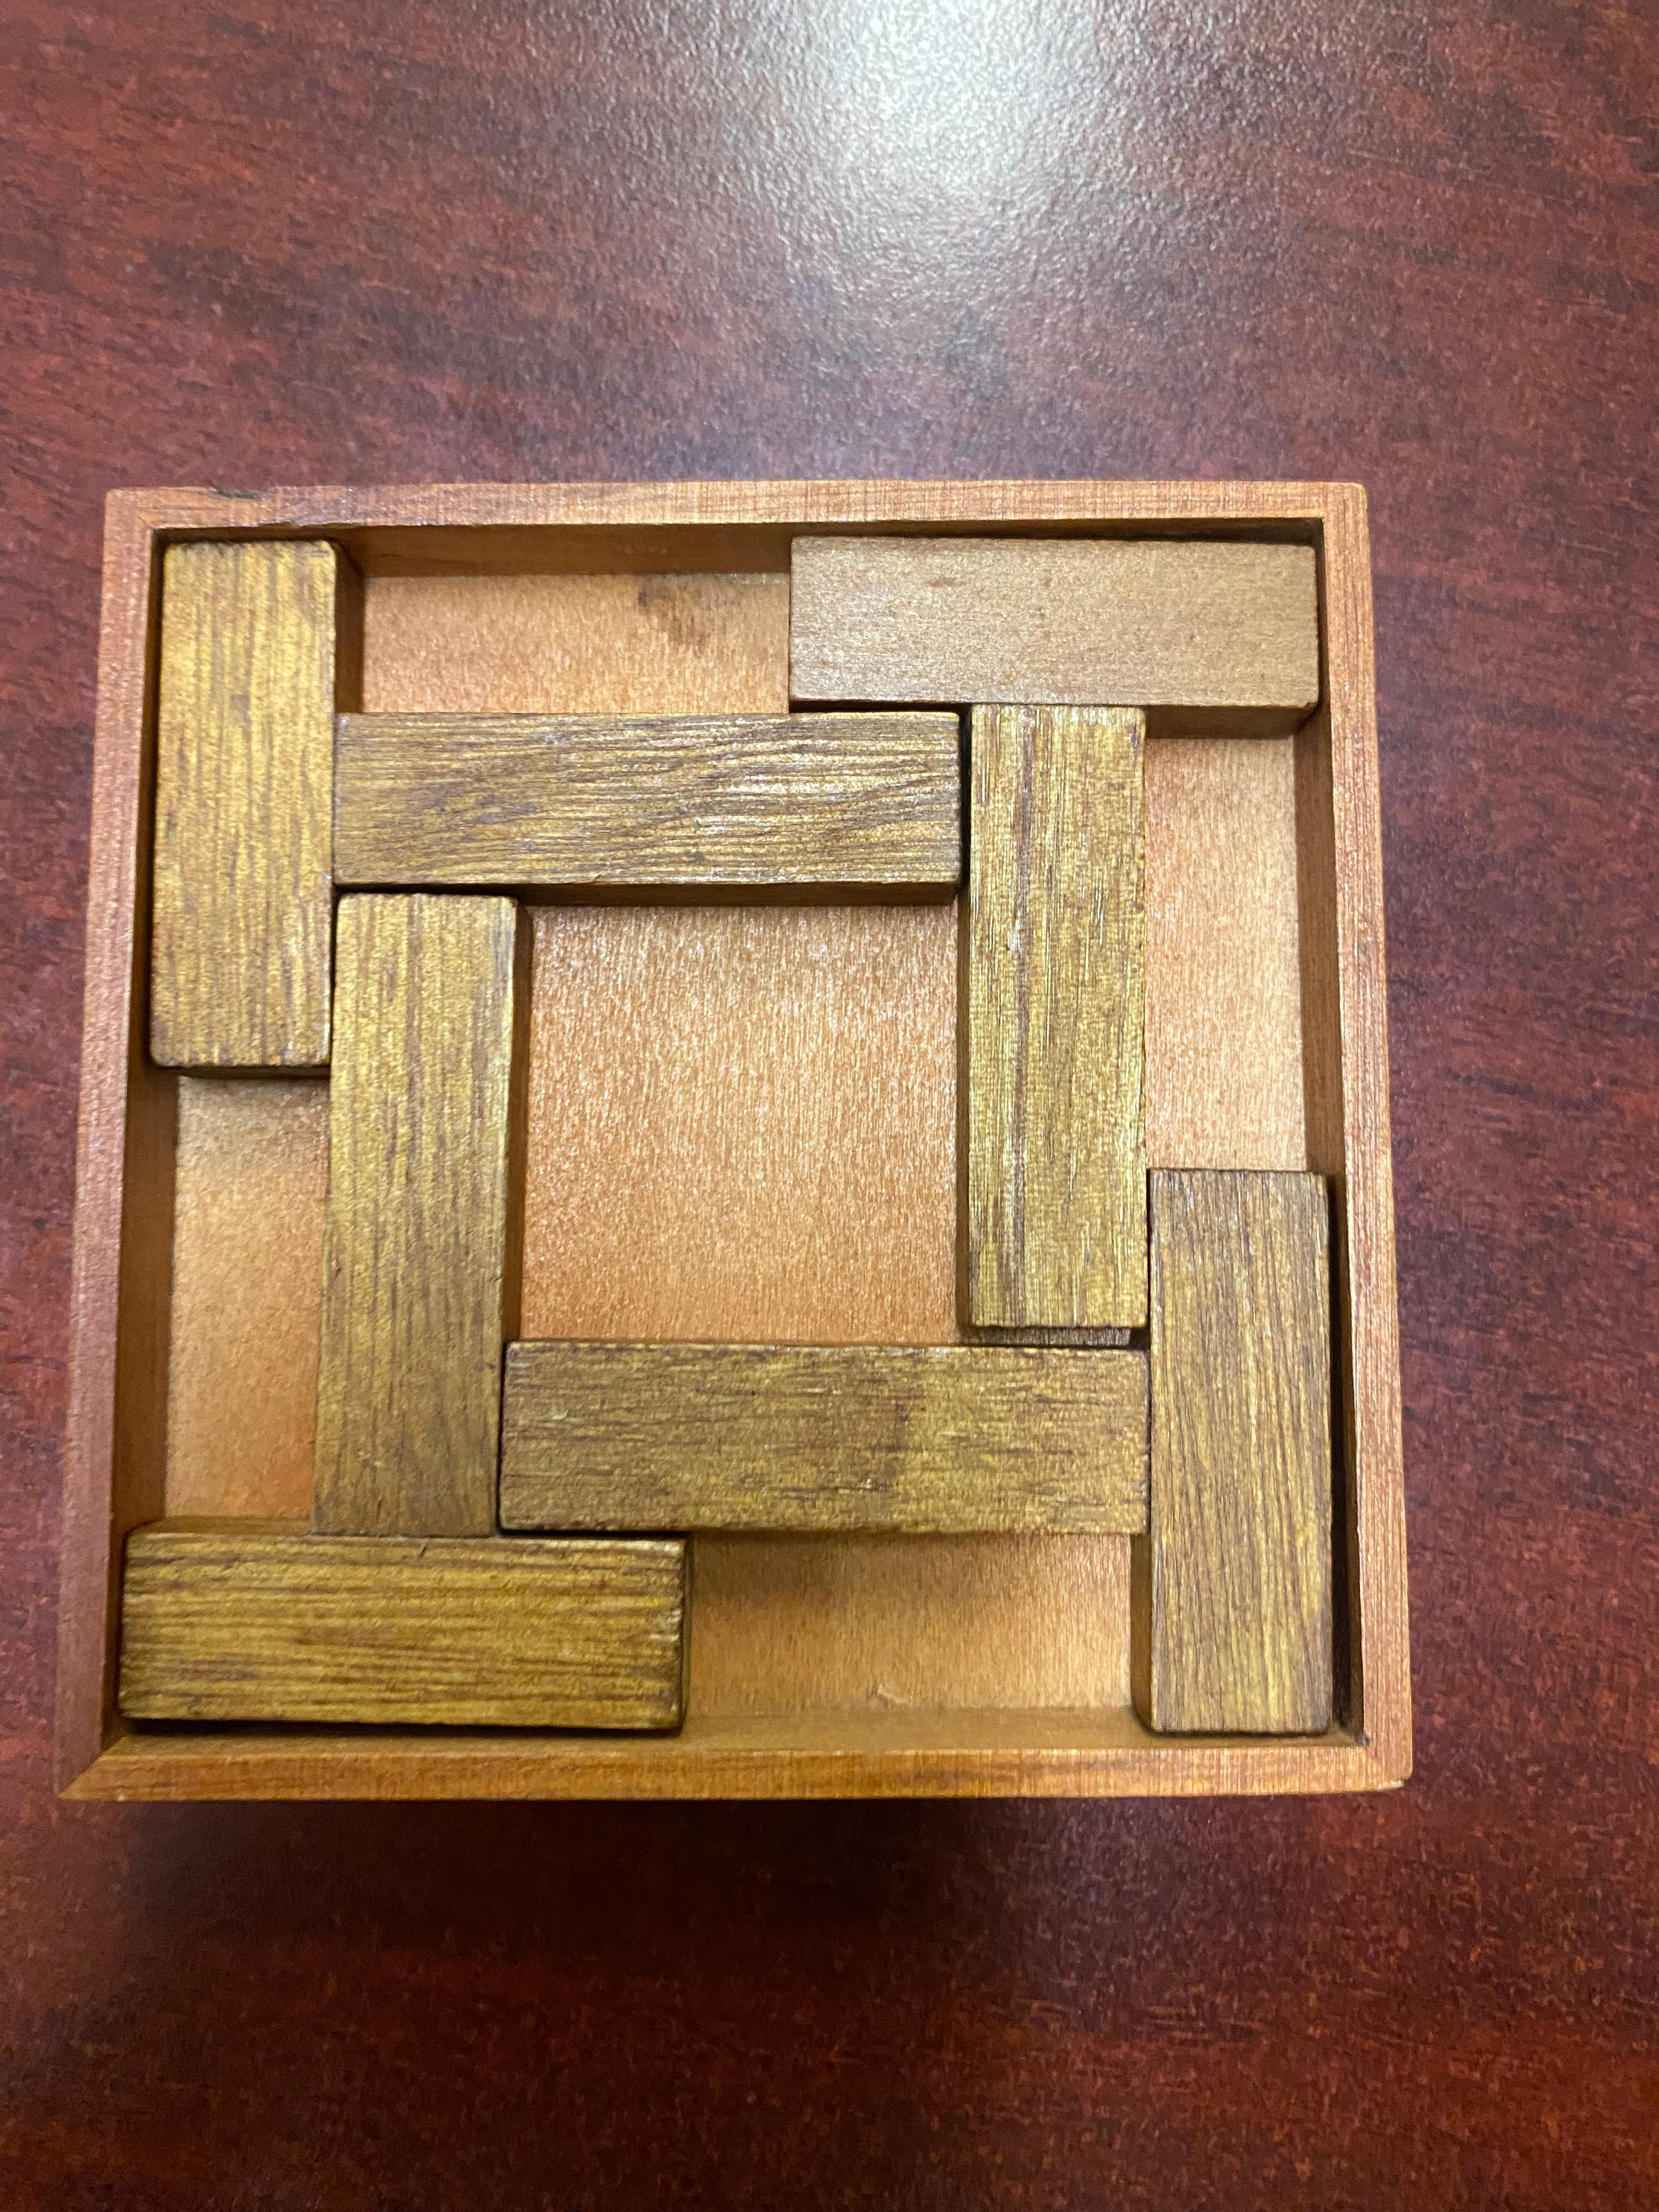
\includegraphics[scale = 0.04]{clase7/R3-Sol2.jpeg}&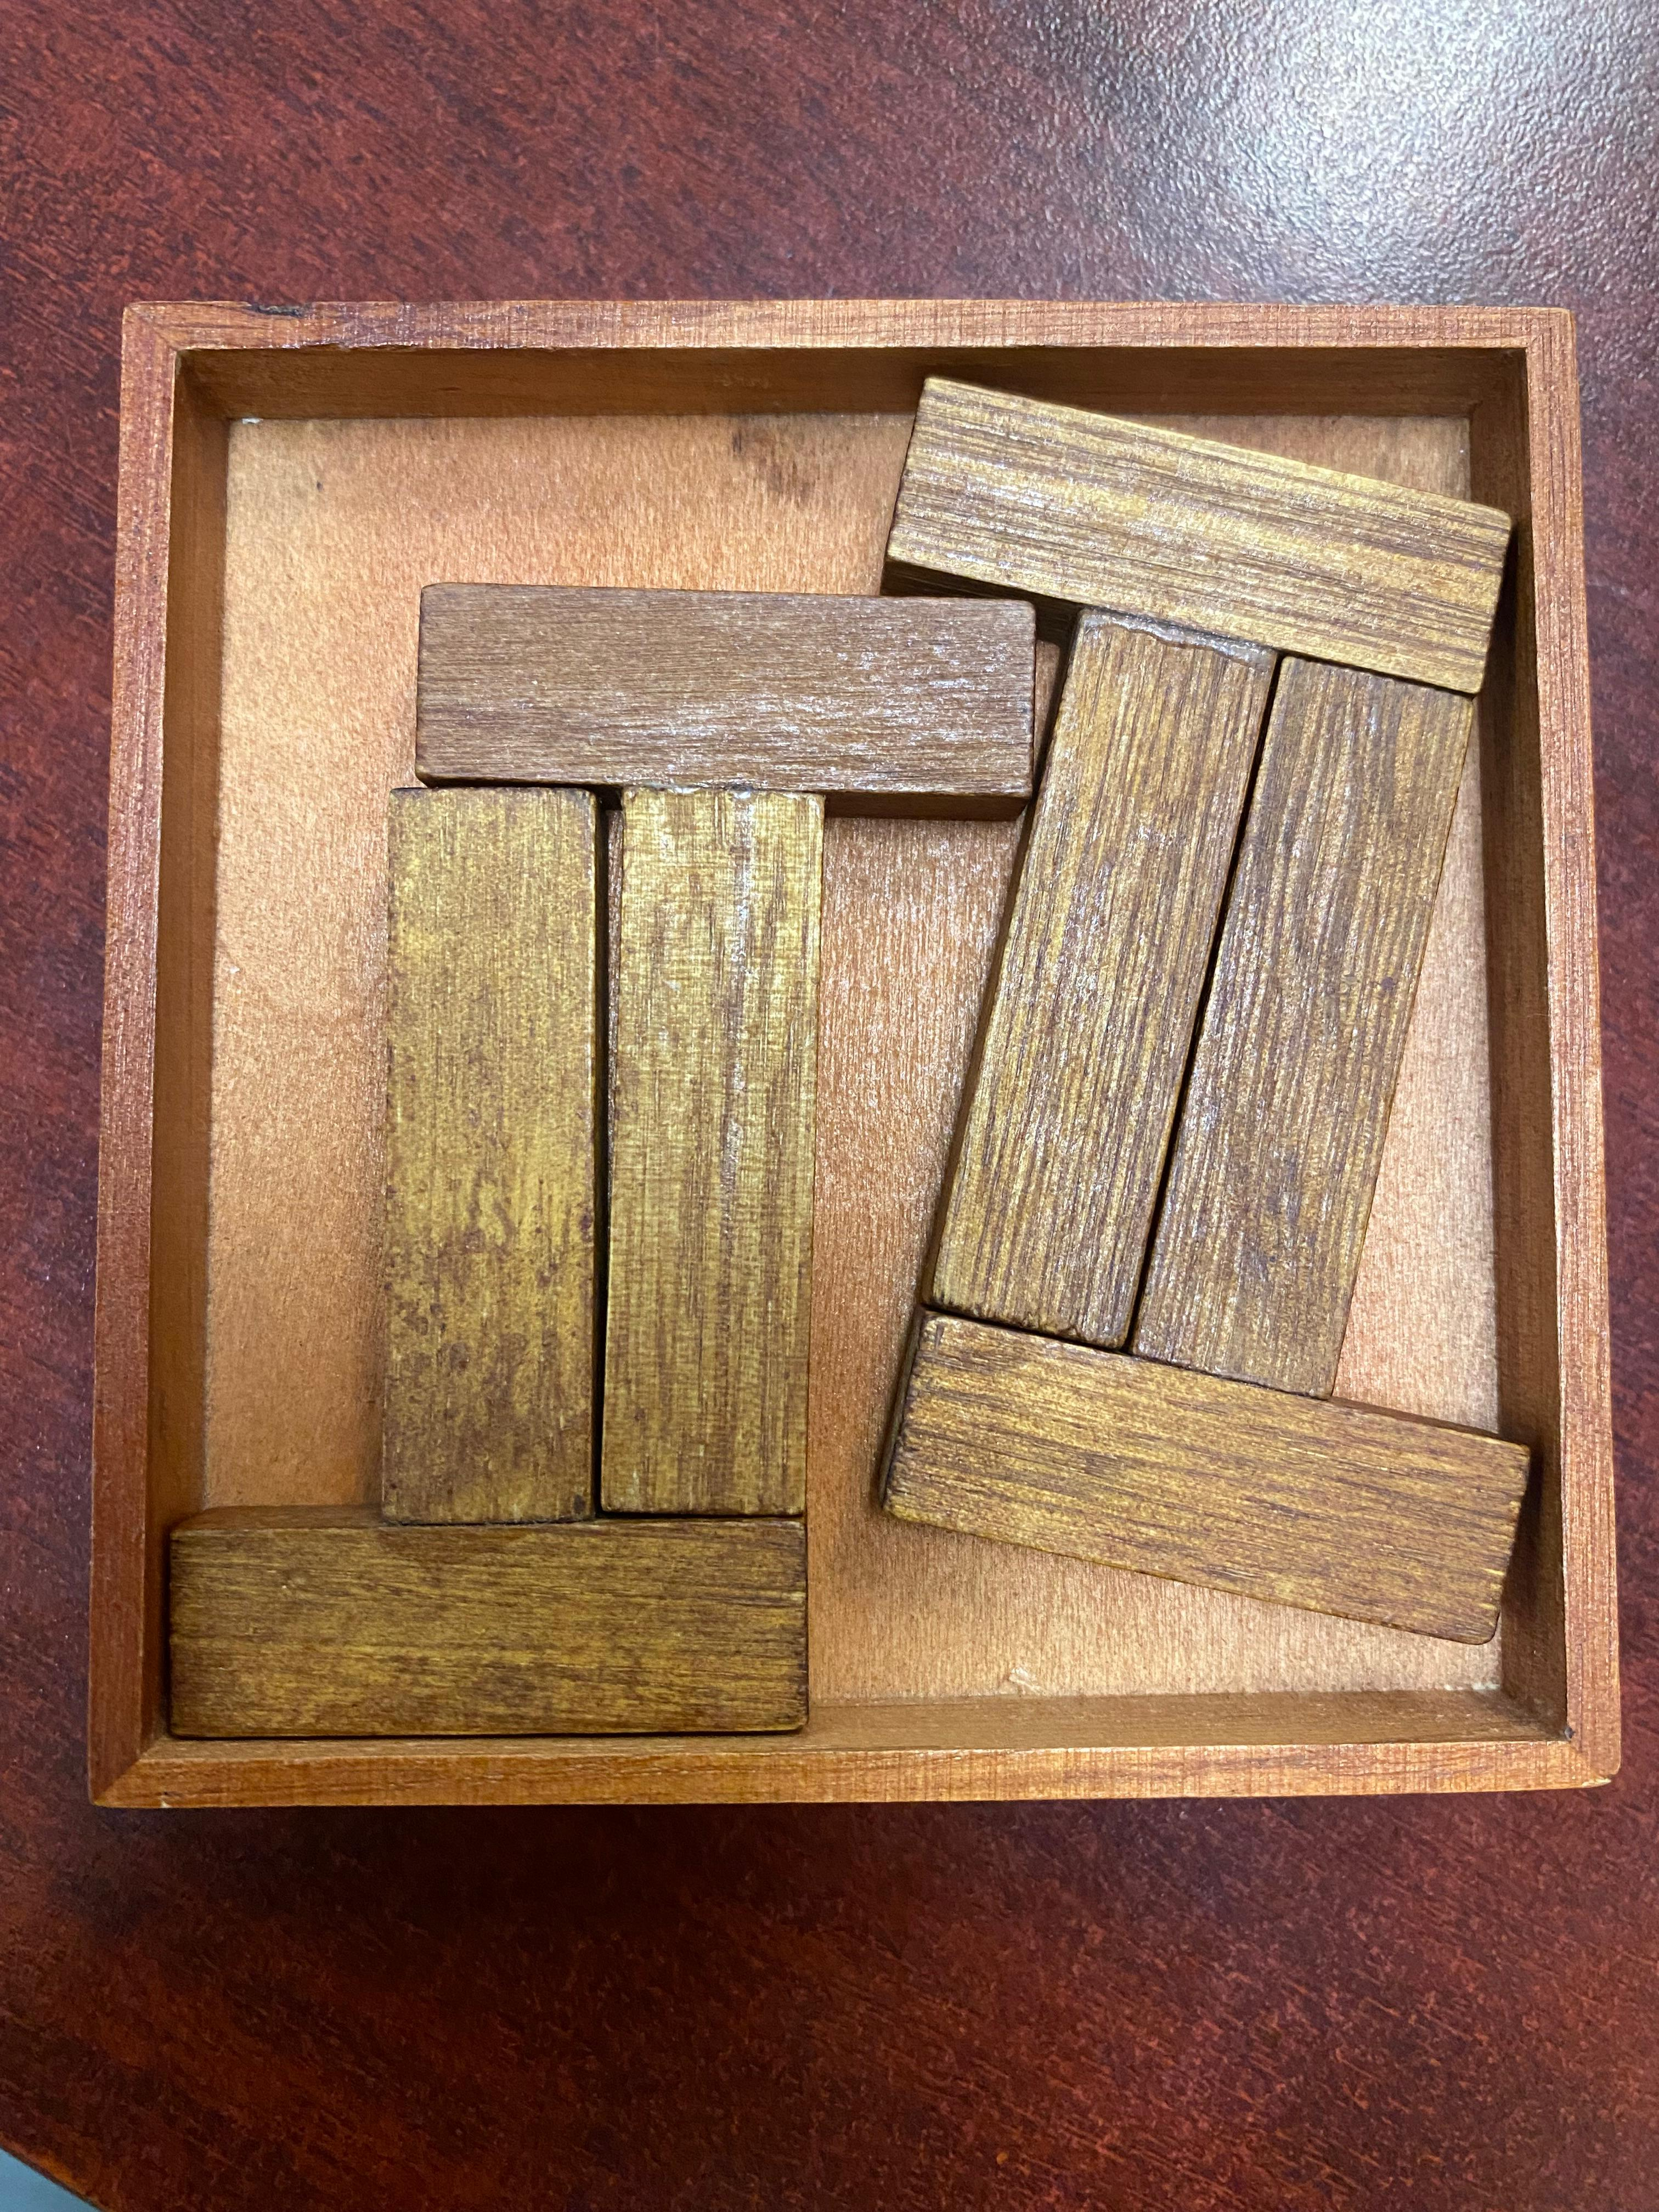
\includegraphics[scale = 0.04]{clase7/R3-Sol3.jpeg}
    \end{tabular}
    \caption{}
\end{figure}
  %\section{Clase 8. Problemas de aritméticos y geométricos}
\textbf{27/02/2025}

%para que concuerde con el número del problemario de pensamiento

\begin{excercise}
    Un tren directo sale de Moscú hacia Leningrado a 90 km por hora. Otro tren directo sale de Leningrado a Moscú a 60 km por hora. ¿A qué distancia están los trenes entre sí media hora antes de que se crucen?
\end{excercise}
\textbf{SOLUCIÓN}
Sea $T_{ML}$ el tren que va de Moscú a Leningrado y $T_{LM}$ el tren que va de Leningrado a Moscú.
Como el problema indica que los dos trenes se cruzan en determinado momento, entonces media hora antes $T_{ML}$ estaba a 45 km del punto en el cual se iba a encontrar con $T_{LM}$, y $T_{LM}$ media hora antes del punto de encuentro con el otro tren estaba 30 km, por lo cual al sumar estas dos distancias, los trenes estaban a 75 km antes de cruzarse. 

\begin{excercise}
    Dos ciclistas empiezan juntos un recorrido de entrenamiento, uno empezando desde Moscú, el otro desde Simferopol. Cuando los ciclistas están separados por 180 millas, una mosca entra en escena. Empezando desde el hombro de uno de los ciclistas, la mosca vuela hasta el otro ciclista. Al llegar al otro, da la vuelta y vuelve. La mosca incansable continúa yendo de uno a otro hasta que los dos se encuentran; entonces se posa sobre la nariz de uno de los ciclistas.
    La velocidad de la mosca es de 30 millas por hora. La velocidad de los ciclistas es de 15 millas por hora. ¿Cuántas millas ha recorrido la mosca?
\end{excercise}
\textbf{SOLUCIÓN}

Cómo cada ciclista individualmente recorre 15 millas por hora, entonces con cada hora la distancia que hay entre ellos dos se reduce en 30 millas. Utilizando la fórmula de velocidad nos da que el tiempo que tardan en encontrarse es de seis horas y como la mosca es capaz de recorrer 30 millas por hora, al multiplicar la cantidad de tiempo que los ciclistas tarden en encontrarse por la velocidad de la mosca nos da que recorre 180 millas, hasta el momento en que los ciclistas se encuentran.

\begin{excercise}
    En 855, el emperador de China Yang Suen tenía que cubrir un puesto importante al que aspiraban dos mandarines de títulos equivalentes. El emperador decidió elegir a aquel que resolviera primero el siguiente problema:
    El jefe de unos bandidos decía a sus hombres: «Hemos robado unas piezas de tela... Si cada uno de nosotros toma seis, quedarán cinco piezas. Pero si cada uno de nosotros quiere siete, nos faltarán ocho.» ¿Cuántos eran los ladrones?
    Como en aquella época no se conocía el álgebra en la China, los mandarines tuvieron que resolver el problema valiéndose de la aritmética. Nosotros nos proponemos hacer lo mismo.
\end{excercise}
\textbf{SOLUCIÓN}

El problema indica que cuando cada ladrón agarra seis pedazos de tela sobran cinco, y al momento de hacer una repartición con un pedazo de tela más, los primeros agarran, los cinco pedazos que sobraron entonces cinco, ya tienen siete pedazos de tela pero hacen falta ocho para que cada uno tenga siete pedazos de tela, por lo cual, si sumamos los 5 pedazos que sobran con los 8 que faltan podemos concluir que son 13 ladrones. 

\begin{excercise}
    Dos coches salen al mismo tiempo del punto A para cumplir una carrera de regularidad. El circuito tiene más de un kilómetro de longitud. Durante toda la competición, en la que darán varias vueltas al circuito, cada coche mantendrá fija su velocidad. Como un coche va más rápido que el otro, en determinados momentos los coches se cruzarán. El primer cruce se produce a 150 metros del punto A. ¿A qué distancia del punto A se cruzarán por segunda vez?
\end{excercise}
\textbf{SOLUCIÓN}
Los coches se volverán a cruzar a 300 m del punto A

\begin{excercise}
    «El café se me enfría » dijo Óscar, «y sigo esperando por la crema y el azúcar.»
    La joven no parecía preocupada.
    «Lo siento, señor » dijo ella. «Voy a traérselos especialmente, ya que la mayoría de la gente nunca los pide aquí.»
    «¿Conque no, eh? Estuve observando a los otros clientes » dijo Óscar « y noté que doce se sirvieron azúcar, siete se sirvieron crema, tres se sirvieron ambas cosas, y únicamente dos no se sirvieron nada.»
    ¿Cuántos clientes además de Óscar había allí?
\end{excercise}
\textbf{SOLUCIÓN}
Con diagramas de ven, primeramente se marcan las intersecciones, es decir, los tres que se sirvieron ambas cosas, y de ahí a la cantidad total de personas que sirvieron crema,, se le resta la intersección, y de igual modo con los que se sirvieron azúcar. Sumando cada cantidad obtenida más las dos personas que no se sirvieron nada, y Oscar nos da un total de 19 personas.
\begin{gather*}
    A : \text{Personas que se sirvieron azúcar} \;
    C : \text{Personas que se sirvieron crema}
\end{gather*}

\begin{center}
    \begin{venndiagram2sets}[labelB = {C}, labelOnlyA = {4}, labelAB = {3}, labelOnlyB = {9}, labelNotAB = {2}]
    \end{venndiagram2sets}
\end{center}


\begin{excercise}
    En la multiplicación que se muestra en la figura, ciertos dígitos han sido reemplazados por un *.
    Encuentra los dígitos que han sido reemplazados por *.
\end{excercise}

\begin{figure*}
    \centering
    \begin{tabular}{c c c c c c | c}
        &&&*&1&*&  1 \\
        &&$\times$&&&&  2 \\
        &&&3&*&2&  3 \\
        \hline
        &&&*&3&*&  4\\
        &3&*&2&*&&  5 \\
        *&2&*&5&&&  6\\
        \hline
        1&*&8&*&3&0&  7\\
        A&B&C&D&E&F \\
    \end{tabular}    
\end{figure*}


\textbf{SOLUCIÓN}

    \begin{center}    
        \begin{tabular}{c c c c c c | c}
            &&&4&1&5&  1 \\
            &&$\times$&&&&  2 \\
            &&&3&8&2&  3 \\
            \hline
            &&&8&3&0&  4\\
            &3&3&2&0&&  5 \\
            1&2&4&5&&&  6\\
            \hline
            1&5&8&5&3&0&  7\\
            A&B&C&D&E&F \\
        \end{tabular}
    \end{center}

Para esta explicación especificaremos el número o asterisco al que nos referimos poniendo por delante su posición entre paréntesis.
El primer paso para hallar el valor de *(F1) fue ver que número del 1-9 multiplicado por 2(F3) podría darme un cero en la posición de las unidades para que concordase con 0(F7), en este caso fue el 5.
Para *(E3) era ver que número multiplicado por 5 tenía una unidad que al ser sumado con la decena de la fila 3 me diera el 3(E7), en este caso habían dos posibilidades, el 4 y el 8. Escogí el 8, pues cumplía otra condición necesaria la cual es que multiplicando 8(E3) $\times$ 1(E3) y sumando la cifra de las decenas de 8(E3)$\times$5(F1) debía terminar en dos. Del mismo modo procedí con los números restantes, observando que números multiplicados por otros tenían cifras que ya conocía en la posición de las unidades.
\\

\begin{excercise}
    Martín estaba tendiendo un alambrado en el fondo del terreno.
    « Me dijiste que pensabas poner los postes con una separación de un metro entre uno y otro» comentó Lucrecia, « pero ahora veo que están más separados».
    «No creí que lo notaras »dijo Martín. « Resulta que me faltaron cuatro postes y tuve que ponerlos a metro y medio uno del otro.»
    ¿Cuánto mide el largo del alambrado?
\end{excercise}

\textbf{SOLUCIÓN}
En la siguiente figura $P$ representa el último poste que se colocó mientras que $Q$ es el final del alambrado y $P_1, P_2, P_3, P_4$ son los postes faltantes

\begin{figure*}[ht!]
    \begin{tikzpicture}
        \draw[<->] (-8,0) -- (6,0);
        %Cada punto representa un poste
        \fill (-6,0) circle (1pt);
        \node[above] at (-6,0) {\footnotesize $P$ };
        
        \fill (-4,0) circle (1pt);
        \node[above] at (-4,0) {\footnotesize $P_1$};
        
        \fill (-2,0) circle (1pt);
        \node[above] at (-2,0) {\footnotesize $P_2$};
        
        \fill (0,0)  circle (1pt);
        \node[above] at (0,0) {\footnotesize $P_3$};
        
        \fill (2,0)  circle (1pt);
        \node[above] at (2,0) {\footnotesize $P_4$};
        
        \fill (4,0)  circle (1pt);
        \node[above] at (4,0) {\footnotesize $Q$};

        %rectas que marcan la distancia entre cada punto
        \draw[<->] (-6,-0.5) -- (-4,-0.5);
        \node at (-5,-1) {\textbf{$1m$}};
        
        \draw[<->] (-4,-0.5) -- (-2,-0.5);
        \node at (-3,-1) {\textbf{$1m$}};
        
        \draw[<->] (-2,-0.5) -- (0,-0.5);
        \node at (-1,-1) {\textbf{$1m$}};
        
        \draw[<->] (0,-0.5) -- (2,-0.5);
        \node at (1,-1) {\textbf{$1m$}};
        
        \draw[<->] (2,-0.5) -- (4,-0.5);
        \node at (3,-1) {\textbf{$1m$}};
    \end{tikzpicture}
\end{figure*}

Notemos que si tenemos 6 postes, la distancia que cubren es de $5m$, de aquí obtenemos la primera ecuación

\begin{gather*}
    l = n-1 \qquad \text{Donde $l:=$ la longitud del alambrado y $n:=$ la cantidad de postes}
\end{gather*}

Pero esto es solo cuando tenemos la cantidad suficiente de postes, como hicieron falta cuatro postes entonces $l = (n-4)-1$ y como la distancia ahora es de $1.5m$ entre cada poste tenemos

\begin{gather*}
    l = \frac{3}{2}(n-5) \\
    \text{Como la longitud del alambrado no cambia entonces podemos igualar ambas ecuaciones}\\
    n-1 = \frac{3}{2}(n-5) \\
    2n-2 = 3n - 15\\
    3n - 2n = 15 -2\\
    n = 13
\end{gather*}

Sustituyendo tenemos $L = 13-1 = 12$, por lo tanto la longitud del alambrado es de $12m$.
  \chapter{Clase 9. PROBLEMAS}
\textbf{04/03/2025}

Ejercicios p.14 del problemario.
\begin{excercise}
    1.13 «Pagué doce centavos por los huevos que compré al tendero», explicó la cocinera, «pero le hice darme dos huevos extra porque eran muy pequeños. Eso hizo que el total sumara un centavo menos por docena que el primer precio que me dio.» ¿Cuántos huevos compró la cocinera?
\end{excercise}

\textbf{SOLUCIÓN}
    $x :=$ Cantidad de huevos comprados inicialmente\\
    $p :=$ Precio inicial de cada huevo\\
    Como una docena vale $12$ centavos entonces
    \[ \frac{12}{\frac{12}{x}} = \frac{144}{x} = P_1 \]
    pero luego le dieron dos, por lo cual
    \[ \frac{12}{\frac{12}{x+2}} = \frac{144}{x+2} = P_2 = P_1 -1 \]
    Luego:\\
    \begin{gather*}
        \\ \frac{12}{\frac{144}{x}}-1 = \frac{144}{x+2}
        \\ \frac{12}{\frac{144-x}{x}} = \frac{144}{x+2}
        \\ (144-x)(x+2) = 144x
        \\ 144x -x^{2} + 288 -2x = 144x
        \\ x^{2}+2x-288 = 0
        \\ x^{2} + 18x -16x - 288 = 0
        \\ x(x+18) -16(x+18) = 0
        \\ (x-16)(x+18); 
        \\ \therefore x_1 = 16, x_2 = -18.
    \end{gather*}
    Descartamos $x_2$ pues buscamos un valor positivo. Así, concluímos que la cocinera compró 18 huevos.

\begin{excercise}
    1.14 La señora Wiggs le explicaba a Lovey Mary que ahora tiene una plantación cuadrada de repollos más grande que la del año pasado, y que por lo tanto tendrá 211 repollos más. ¿Cuántos repollos tendrá este año la señora Wiggs.
\end{excercise}

\textbf{SOLUCIÓN}
\begin{center}
    \begin{tikzpicture}
    %cuadrado m
    \draw (0,5) -- (5,5) -- (5,0) -- (0,0) --cycle; %Cuadrado m
    \draw[<->] (5.5,0) -- (5.5,5); %Linea que marca longitud m
    \node (m) at (5.9,2.5) {m}; %Etiqueta de l_m
    \node (mpow) at (4,2.5) {$m^{2}$};%label cuad m

    
    %Cuadrado n
    \draw (0,2.5) -- (2.5,2.5) -- (2.5,5); %Cuadrado
    \draw[<->] (3,2.5) -- (3,5); %Linea que marca longitud n
    \node (n) at (3.4,3.7) {n}; %Etiqueta de l_n
    \node (npow) at (1.7,3.7) {$n^{2}$}; %Label cuad n
\end{tikzpicture}
\end{center}
Notemos que:
\begin{gather*}
    m^{2} = n^{2} + 211 \Rightarrow m^{2} - n^{2} = 211
    \\ (m+n)(m-n) = 211
\end{gather*}
Como 211 es un número primo, entonces
\begin{equation*}
    \begin{aligned}
        m-n = 1\\
        m+n = 211
    \end{aligned}
\end{equation*}
Sumando obtenemos $2m = 212 \Rightarrow m = 106$\\
Sustituyendo $m$ en $m+n = 211 \quad \Rightarrow n =105$ \\

Ahora, $106^{2} = 11236$ y esta es la cantidad de repollos que tendrá la señora Wiggs este año.

\begin{excercise}
    1.15 Tras recoger 770 castañas, tres niñas las dividieron de modo que las cantidades recibidas guardaran la misma proporción que sus edades. Cada vez que Mary se quedaba con cuatro castañas, Nellie tomaba tres, y por cada seis que recibía Mary, Susie tomaba siete. ¿Cuántas castañas recibió cada niña?
\end{excercise}

\textbf{SOLUCION}
Definimos $M,N,S$ a las castañas que le corresponden a Mary, Nellie y a Susie, respectivamente. Entonces $M:N :: M:S\text{ equivalente a } 4:3 :: 6:7$
\begin{gather*}
    \frac{M}{N} = \frac{3}{4} \rightarrow N = \frac{3}{4}M \\
    \frac{M}{S} = \frac{7}{6} \rightarrow S = \frac{7}{6}M \\
\end{gather*}
Pero $M+N+S = 770$
\begin{gather*}
    M + \frac{3}{4}M + \frac{7}{6}M = 770 \\
    \frac{35M}{12} = 770 \\
    M = \frac{770 \cdot 12}{35} \rightarrow M = 264\\
\end{gather*}
Luego
\begin{gather*}
    N = \frac{3}{4}M \rightarrow N = 198\\
    S = \frac{7}{6}M \rightarrow S = 308\\
\end{gather*}
Mary, Nellie y Susie tiene 264, 198 y 308 castañas, respectivamente.
  % \chapter{Clase 10. Configuraciones geométricas}
\textbf{05/03/2025}

\section{Problemas p.14 del problemario}

\begin{tabular}{l c}
    Problema & Solución \\\hline
    
    Tienes 9 puntos acomodados en 3 filas con 3 con tres puntos cada fila, formando un cuadrado. Sin levantar el lápiz, dibuja 4 segmentos de recta que pase por los 9 puntos. & lorem
\end{tabular}


\begin{excercise}
    Acomoda 9 puntos en 6 filas y cada fila con 3 puntos.
\end{excercise}

\begin{excercise}
    Acomoda 10 puntos en 5 filas y cada fila con 4 puntos.
\end{excercise}

\section{Problemas p.15 del problemario}

\end{document}
